% ============================================================
%  Ripple — 腾讯 PCG 校园 AI 产品创意大赛 竞赛技术报告
%  作者：戴尚好  中国科学技术大学
%  编译：tectonic -X compile ripple_report_v4.tex
% ============================================================
%
%  【截图替换指南】
%  运行产品后 (http://localhost:5173)，截图放入 pdf/screenshots/ 目录：
%    hero.png          — 首屏 5 秒法则着陆页（全宽截图）
%    content_eco.png   — 内容生态图展开状态（全宽截图）
%    roundtable.png    — AI 圆桌 7 位专家发言中（全宽截图）
%    ces_dash.png      — CES 仪表盘雷达图+增长曲线（全宽截图）
%    ces_slider.png    — CES 滑块实时调节（半宽截图）
%    wechat_search.png — 搜一搜关键词热度柱状图（半宽截图）
%    wechat_video.png  — 视频号社交链路图（半宽截图）
%    koc_diagnose.png  — KOC 四阶段诊断（全宽截图）
%    copy_export.png   — 多格式一键复制（半宽截图）
%    demo_cases.png    — Demo 案例列表首屏（全宽截图）
%  截图后将上方占位框 \fbox{...} 替换为 \includegraphics[...]{screenshots/xxx.png}
% ============================================================

\documentclass[12pt,a4paper]{ctexart}

% ── 基础宏包 ────────────────────────────────────────────────
\usepackage{geometry}
\geometry{left=2.5cm,right=2.5cm,top=3cm,bottom=3cm}
\usepackage{amsmath}
\usepackage{amssymb}
\usepackage{graphicx}
\usepackage{xcolor}
\usepackage{tcolorbox}
\tcbuselibrary{skins,breakable}
\usepackage{booktabs}
\usepackage{tabularx}
\usepackage{array}
\usepackage{multirow}
\usepackage{longtable}
\usepackage{tikz}
\usetikzlibrary{shapes.geometric,arrows.meta,positioning,fit,
                backgrounds,calc,decorations.pathmorphing,shadows}
\usepackage{pgfplots}
\pgfplotsset{compat=1.18}
\usepackage{hyperref}
\hypersetup{colorlinks=true,linkcolor=primary,urlcolor=primary,citecolor=primary}
\usepackage{titlesec}
\usepackage{enumitem}
\usepackage{microtype}
\usepackage{fancyhdr}
\usepackage{setspace}
\usepackage{caption}
\usepackage{subcaption}
\usepackage{listings}
\usepackage{fontawesome5}
\usepackage{mdframed}
\usepackage{pifont}
\usepackage{wasysym}

% ── 颜色定义 ────────────────────────────────────────────────
\definecolor{primary}{HTML}{3B82F6}
\definecolor{secondary}{HTML}{8B5CF6}
\definecolor{accent}{HTML}{06B6D4}
\definecolor{success}{HTML}{10B981}
\definecolor{warning}{HTML}{F59E0B}
\definecolor{danger}{HTML}{EF4444}
\definecolor{darkbg}{HTML}{1E293B}
\definecolor{lightbg}{HTML}{F8FAFC}
\definecolor{codebg}{HTML}{F1F5F9}
\definecolor{border}{HTML}{E2E8F0}
\definecolor{textmuted}{HTML}{64748B}
\definecolor{ripple1}{HTML}{BFDBFE}
\definecolor{ripple2}{HTML}{93C5FD}
\definecolor{ripple3}{HTML}{60A5FA}

% ── 章节标题样式 ─────────────────────────────────────────────
\titleformat{\section}[block]
  {\Large\bfseries\color{primary}}
  {\thesection}{0.6em}{}
  [\vspace{-0.4em}{\color{primary}\rule{\linewidth}{1.2pt}}]

\titleformat{\subsection}[block]
  {\large\bfseries\color{darkbg}}
  {\thesubsection}{0.5em}{}

\titleformat{\subsubsection}[block]
  {\normalsize\bfseries\color{secondary}}
  {\thesubsubsection}{0.5em}{}

% ── 代码块样式 ───────────────────────────────────────────────
\lstdefinestyle{pycode}{
  language=Python,
  basicstyle=\ttfamily\small,
  keywordstyle=\color{primary}\bfseries,
  stringstyle=\color{success},
  commentstyle=\color{textmuted}\itshape,
  numbers=left,
  numberstyle=\tiny\color{textmuted},
  numbersep=8pt,
  frame=single,
  frameround=tttt,
  rulecolor=\color{border},
  backgroundcolor=\color{codebg},
  breaklines=true,
  breakatwhitespace=false,
  tabsize=4,
  showstringspaces=false,
  xleftmargin=12pt,
}

% ── tcolorbox 快捷框 ─────────────────────────────────────────
\newenvironment{keybox}[1]{%
  \begin{tcolorbox}[colback=primary!8,colframe=primary,
    title={\textbf{#1}},fonttitle=\color{white}\bfseries,
    coltitle=white,left=6pt,right=6pt,top=4pt,bottom=4pt,
    arc=4pt]
}{%
  \end{tcolorbox}
  \vspace{0.3cm}
}

\newenvironment{innobox}[1]{%
  \begin{tcolorbox}[colback=secondary!8,colframe=secondary,
    title={\textbf{[创新] #1}},fonttitle=\color{white}\bfseries,
    coltitle=white,left=6pt,right=6pt,top=4pt,bottom=4pt,arc=4pt]
}{%
  \end{tcolorbox}
  \vspace{0.3cm}
}

\newenvironment{techbox}[1]{%
  \begin{tcolorbox}[colback=accent!8,colframe=accent,
    title={\textbf{[技术] #1}},fonttitle=\color{white}\bfseries,
    coltitle=white,left=6pt,right=6pt,top=4pt,bottom=4pt,arc=4pt]
}{%
  \end{tcolorbox}
  \vspace{0.3cm}
}

\newenvironment{warnbox}[1]{%
  \begin{tcolorbox}[colback=warning!10,colframe=warning,
    title={\textbf{#1}},fonttitle=\color{white}\bfseries,
    coltitle=white,left=6pt,right=6pt,top=4pt,bottom=4pt,arc=4pt]
}{%
  \end{tcolorbox}
  \vspace{0.3cm}
}

% ── 图片占位符命令 ───────────────────────────────────────────
\newcommand{\imgplaceholder}[2]{%
  \begin{center}
    \fbox{\parbox[c][4.5cm][c]{#1}{%
      \centering
      \color{textmuted}
      \large [截图占位]\\[0.3cm]
      \normalsize #2\\[0.2cm]
      \small 请将对应截图放入 pdf/screenshots/ 后替换
    }}
  \end{center}
}

\newcommand{\imgplaceholdersm}[2]{%
  \begin{center}
    \fbox{\parbox[c][3cm][c]{#1}{%
      \centering\color{textmuted}\normalsize [截图占位]\\ #2
    }}
  \end{center}
}

% ── 页眉页脚 ─────────────────────────────────────────────────
\pagestyle{fancy}
\fancyhf{}
\fancyhead[L]{\color{textmuted}\small\textbf{Ripple} — KOC 内容增长 AI 平台}
\fancyhead[R]{\color{textmuted}\small 腾讯 PCG 校园 AI 产品创意大赛}
\fancyfoot[C]{\color{textmuted}\small\thepage}
\renewcommand{\headrulewidth}{0.4pt}
\renewcommand{\headrule}{\color{border}\hrule width\headwidth height\headrulewidth}

% ── 行距 ─────────────────────────────────────────────────────
\setstretch{1.25}

% ── 列表样式 ─────────────────────────────────────────────────
\setlist[itemize]{leftmargin=1.5em,itemsep=2pt,topsep=4pt}
\setlist[enumerate]{leftmargin=1.5em,itemsep=2pt,topsep=4pt}

% ============================================================
\begin{document}
% ============================================================


% ============================================================
%  封面页 1：品牌封面
% ============================================================
\begin{titlepage}
\thispagestyle{empty}

% 背景色块
\begin{tikzpicture}[remember picture,overlay]
  \fill[darkbg] (current page.south west) rectangle (current page.north east);
  % 波纹装饰
  \foreach \r/\op in {3/0.08, 5/0.06, 7/0.05, 9/0.04, 11/0.03, 13/0.02}{
    \draw[primary,opacity=\op,line width=1.5pt]
      (current page.center) circle (\r cm);
  }
  \fill[primary,opacity=0.15] (current page.center) circle (2.5cm);
  \fill[primary,opacity=0.25] (current page.center) circle (1.5cm);
  \fill[white,opacity=0.9]    (current page.center) circle (1.0cm);
\end{tikzpicture}

\vspace*{5cm}
\begin{center}
  {\fontsize{18pt}{22pt}\selectfont\color{ripple1}\textbf{Ripple}}\\[0.3cm]
  {\fontsize{52pt}{60pt}\selectfont\color{white}\textbf{Ripple}}\\[0.1cm]
  {\fontsize{16pt}{20pt}\selectfont\color{ripple2}波 纹}\\[1.2cm]

  
\begin{tikzpicture}
    \draw[ripple2,line width=0.8pt] (0,0) -- (10cm,0);
  \end{tikzpicture}\\[0.8cm]

  {\fontsize{18pt}{24pt}\selectfont\color{white}
    \textbf{把 60 秒的内容直觉，变成 5 分钟的可执行方案}}\\[0.6cm]
  {\fontsize{13pt}{18pt}\selectfont\color{ripple1}
    AI 驱动的大学生 KOC 内容增长引擎}\\[0.4cm]
  {\fontsize{11pt}{16pt}\selectfont\color{textmuted}
    小红书 $\cdot$ 微信视频号 $\cdot$ 搜一搜 $\cdot$ 公众号 全生态覆盖}\\[2cm]

  
\begin{tikzpicture}
    \draw[ripple2,opacity=0.5,line width=0.8pt] (0,0) -- (8cm,0);
  \end{tikzpicture}\\[0.8cm]

  {\fontsize{12pt}{16pt}\selectfont\color{ripple2}
    腾讯 PCG 校园 AI 产品创意大赛参赛作品}\\[0.3cm]
  {\fontsize{11pt}{15pt}\selectfont\color{textmuted}2026 年 5 月}
\end{center}
\end{titlepage}


% ============================================================
%  封面页 2：作者与竞赛信息
% ============================================================
\newpage
\thispagestyle{empty}
\vspace*{2cm}

\begin{center}
{\LARGE\bfseries\color{primary} 参赛信息与作者介绍}
\vspace{0.3cm}
\textcolor{primary}{\rule{12cm}{1.2pt}}
\end{center}

\vspace{1cm}

\begin{tcolorbox}[colback=lightbg,colframe=primary,arc=6pt,
  left=12pt,right=12pt,top=10pt,bottom=10pt]
\begin{center}
{\large\bfseries\color{primary} 参赛信息}
\end{center}
\vspace{0.3cm}

\begin{tabular}{p{3.5cm} p{10cm}}
\textbf{赛事名称} & 腾讯 PCG 校园 AI 产品创意大赛 \\[4pt]
\textbf{赛题方向} & 赛题 5：帮助 KOC 轻松涨粉 \\[4pt]
\textbf{产品名称} & Ripple（波纹）\\[4pt]
\textbf{产品定位} & 面向大学生 KOC 的 AI 内容增长全流程助手 \\[4pt]
\textbf{技术特色} & 腾讯混元 LLM + 多 Agent 协同 + 实时可视化分析 \\[4pt]
\textbf{提交日期} & 2026 年 5 月 6 日 \\
\end{tabular}
\end{tcolorbox}

\vspace{0.8cm}

\begin{tcolorbox}[colback=lightbg,colframe=secondary,arc=6pt,
  left=12pt,right=12pt,top=10pt,bottom=10pt]
\begin{center}
{\large\bfseries\color{secondary} 作者信息}
\end{center}
\vspace{0.3cm}

\begin{tabular}{p{3.5cm} p{10cm}}
\textbf{姓名} & 戴尚好 \\[4pt]
\textbf{院校} & 中国科学技术大学（在读硕士）\\[4pt]
\textbf{邮箱} & \href{mailto:bcefghj@163.com}{bcefghj@163.com} \\[4pt]
\textbf{手机} & 13296886603 \\[4pt]
\textbf{个人主页} & \url{https://bcefghj.github.io/} \\[4pt]
\textbf{GitHub} & \url{https://github.com/bcefghj}（1400+ Stars，55+ 项目）\\[4pt]
\textbf{Ripple 项目} & \url{https://github.com/bcefghj/ripple} \\[4pt]
\textbf{在线演示} & \url{http://120.55.247.6/} （官网 + Demo）\\[4pt]
\textbf{小红书} & bcefghj（1.6 万粉丝，AI/Agent 技术分享）\\[4pt]
\textbf{研究方向} & Multi-Agent 系统架构 / RAG / MCP 协议 / LLM 推理优化 \\
\end{tabular}
\end{tcolorbox}

\vspace{0.8cm}

\begin{tcolorbox}[colback=primary!5,colframe=primary!30,arc=6pt,
  left=12pt,right=12pt,top=8pt,bottom=8pt]
\begin{center}
\textbf{核心技术亮点速览}
\end{center}
\vspace{0.2cm}
\begin{tabular}{p{1.2cm} p{4cm} p{1.2cm} p{4cm} p{1.2cm} p{3cm}}
(AI) & 7 位 AI 专家圆桌 &
(CES) & CES 爆款指数模拟 &
(KG) & 内容生态图谱 \\[4pt]
(KOC) & KOC 4 阶段诊断 &
(WX) & 微信生态四面板 &
(SSE) & 全链路流式 \\
\end{tabular}
\end{tcolorbox}

\vspace*{\fill}
\begin{center}
\small\color{textmuted}
本报告基于 Ripple v3 实现，代码库包含 React 19 前端 + FastAPI 后端，完整可运行。\\
GitHub 仓库 / 本地启动详见附录 C。
\end{center}


% ============================================================
%  目录
% ============================================================
\newpage
\tableofcontents
\newpage


% ============================================================
%  执行摘要
% ============================================================
\section*{执行摘要}
\addcontentsline{toc}{section}{执行摘要}

\begin{tcolorbox}[colback=primary!6,colframe=primary,arc=5pt,
  left=10pt,right=10pt,top=8pt,bottom=8pt]
\textbf{Ripple}（波纹）是一款面向大学生 KOC 群体的 AI 原生内容增长平台。
核心价值主张：\textbf{``把 60 秒的内容直觉，变成 5 分钟的可执行方案''}。
平台深度整合腾讯混元大模型，提供从选题研究、内容评估、多平台策略到一键发布的完整 AI 闭环。
\end{tcolorbox}

\vspace{0.3cm}
\textbf{五维度竞赛自评：}

\begin{center}
\begin{tabular}{p{3cm} p{1.2cm} p{10cm}}
\toprule
\textbf{评分维度} & \textbf{分值} & \textbf{核心亮点} \\
\midrule
创新性 & 25 分 & 7 位 AI 专家圆桌可视化（业界首创）、CES 算法模拟器、KOC 阶段诊断 \\[3pt]
技术实现 & 25 分 & 腾讯混元深度集成、React 19 + FastAPI 全异步、SSE 流式、60 节点生态图 \\[3pt]
用户体验 & 20 分 & 5 秒法则首屏、6 个零延迟 Demo、多平台一键导出、移动端全适配 \\[3pt]
商业价值 & 15 分 & 1000 万+ 大学生 KOC 市场、腾讯生态深度协同、SaaS 订阅双轨道 \\[3pt]
展示效果 & 15 分 & 19 维雷达图、增长曲线、流量池预测、7 张高质量产品截图 \\
\bottomrule
\end{tabular}
\end{center}

\vspace{0.3cm}
\textbf{核心差异化（vs. ChatGPT / Perplexity）：}
Ripple 不是``会回答 KOC 问题的 AI''，而是``用算法模拟和可视化让 KOC 能直接行动的产品''。
七大独家 AI 原生能力（详见第一部分）使产品具备高护城河，不可被通用 AI 简单替代。


% ============================================================
%  PART 1  创新性
% ============================================================
\newpage
\begin{center}
\begin{tikzpicture}
  \fill[primary!15,rounded corners=8pt] (0,0) rectangle (15cm,1.8cm);
  \node[anchor=west] at (0.5cm,0.9cm)
    {\LARGE\bfseries\color{primary} Part 1\quad 创新性};
  \node[anchor=east] at (14.5cm,0.9cm)
    {\Large\bfseries\color{primary!70} 25 分};
\end{tikzpicture}
\end{center}

\section{大学生 KOC 市场痛点深度分析}

\subsection{目标用户群体画像}

大学生 KOC（Key Opinion Consumer，关键意见消费者）是指在社交媒体上凭借真实内容影响消费决策的普通用户群体。
不同于专业 MCN 旗下的 KOL（Key Opinion Leader），大学生 KOC 具有以下典型特征：

\begin{itemize}
  \item \textbf{内容创作经验匮乏}：缺乏系统的内容策划、平台算法知识和发布技巧
  \item \textbf{时间资源有限}：学业与创作并行，每天可投入的内容创作时间仅 1-3 小时
  \item \textbf{增长瓶颈明显}：通常在 0$\rightarrow$1000 粉阶段停滞最久，缺乏科学的突破路径
  \item \textbf{平台规则陌生}：对小红书 CES 算法、视频号社交链路、公众号 SEO 等机制了解甚少
  \item \textbf{选题决策困难}：凭直觉选题，缺乏数据支撑，导致大量内容``石沉大海''
  \item \textbf{多平台协同复杂}：在小红书、微信视频号、公众号之间切换运营效率极低
\end{itemize}

\subsection{市场调研与痛点量化}

根据 2025 年内容创作行业报告及用户访谈，大学生 KOC 群体面临以下核心痛点：

\begin{center}
{\small
\begin{tabular}{p{3.5cm} p{5cm} p{5.5cm}}
\toprule
\textbf{痛点类型} & \textbf{具体表现} & \textbf{Ripple 解决方案} \\
\midrule
不知道做什么内容 & 每次选题靠碰运气，内容方向摇摆 & 领域雷达扫描 + 6 大维度评分选题 \\[3pt]
不知道能不能爆 & 发出去才知道效果，没有预判能力 & CES 爆款指数模拟器，发前评分 \\[3pt]
不理解平台算法 & 微信视频号/搜一搜规则如天书 & 4 个可视化交互面板直接秒懂 \\[3pt]
AI 推荐不可信 & 单一 AI 建议缺乏对抗性验证 & 7 位专家多角度圆桌讨论 \\[3pt]
内容发布效率低 & 手动改写多个平台格式耗时 & 一键复制 4 种平台格式 \\[3pt]
增长路径不清晰 & 不知道自己处于哪个阶段 & KOC 四阶段诊断 + 专属建议 \\[3pt]
等待时间过长 & AI 分析需要等待 60+ 秒 & SSE 流式输出 + 6 个零延迟 Demo \\
\bottomrule
\end{tabular}
}
\end{center}

\subsection{KOC 增长的关键障碍分析}

\begin{keybox}{为什么大学生 KOC 在 0-1000 粉阶段最难突破？}
\begin{enumerate}
  \item \textbf{冷启动流量池极小}：小红书对新账号的首次曝光仅 100-500 次，CTR $\geq$ 3\% 才能进入下一流量池
  \item \textbf{平台算法不透明}：CES 算法（关注$\times$8 + 评论$\times$4 + 转发$\times$4 + 收藏$\times$1 + 点赞$\times$1）不为大众所知
  \item \textbf{选题竞争激烈}：热门赛道头部内容占据 80\% 流量，新手需找到``蓝海''角度
  \item \textbf{多平台策略割裂}：视频号依赖社交关系链（权重 60\%），与小红书搜索逻辑完全不同
  \item \textbf{内容质量判断难}：无工具评估标题吸引力、Hook 强度、信息密度等关键指标
\end{enumerate}
\end{keybox}


\section{现有产品调研与竞品对比}

\subsection{市场现有解决方案的局限性}

目前市场上针对 KOC 涨粉需求的工具主要分为以下三类，均存在明显局限：

\textbf{（1）通用 AI 对话工具（ChatGPT / 文心一言 / Kimi）}

这类工具虽然可以回答关于内容创作的问题，但本质上是通用问答工具，缺乏：
\begin{itemize}
  \item 平台算法模拟能力（无法真正计算 CES 分数）
  \item 结构化可视化（无法生成内容生态图、增长曲线）
  \item 实时数据检索（缺乏当前热点感知能力）
  \item 多 Agent 对抗性验证（单一视角容易产生偏差建议）
\end{itemize}

\textbf{（2）数据分析工具（蝉妈妈 / 新红 / 飞瓜）}

专业的数据工具提供竞品分析和热词监测，但：
\begin{itemize}
  \item 面向专业运营人员，大学生学习门槛极高
  \item 提供数据不提供行动建议，仍需人工分析转化
  \item 不集成内容创作流程，无法从分析直接到执行
  \item 月费 500-2000 元，大学生难以承担
\end{itemize}

\textbf{（3）内容生成工具（即梦 / 可灵 / 豆包）}

专注于内容生成但缺乏策略支持：
\begin{itemize}
  \item 只管生产内容，不管内容是否能传播
  \item 缺乏选题决策支持和效果预测能力
  \item 无法解决``做什么内容''的根本困惑
\end{itemize}

\subsection{核心竞品差异化对比表}

\begin{center}
{\small
\begin{tabular}{>{\raggedright\arraybackslash}p{4.5cm}
                >{\centering\arraybackslash}p{2cm}
                >{\centering\arraybackslash}p{2.5cm}
                >{\centering\arraybackslash}p{2.5cm}
                >{\centering\arraybackslash}p{2cm}}
\toprule
\textbf{功能维度} & \textbf{ChatGPT} & \textbf{Perplexity} & \textbf{专业数工具} & \textbf{Ripple} \\
\midrule
多源实时搜索 + 引用 & 部分 & (OK) & (OK) & (OK) \\[2pt]
7 位 AI 专家圆桌辩论 & (--) & (--) & (--) & \textbf{[OK]} \\[2pt]
CES 爆款指数模拟器 & (--) & (--) & 部分 & \textbf{[OK]} \\[2pt]
KOC 4 阶段诊断 & (--) & (--) & (--) & \textbf{[OK]} \\[2pt]
视频号社交链路可视化 & (--) & (--) & 部分 & \textbf{[OK]} \\[2pt]
内容生态图谱 & (--) & (--) & 部分 & \textbf{[OK]} \\[2pt]
微信生态 4 大子系统 & (--) & (--) & (--) & \textbf{[OK]} \\[2pt]
多平台格式一键转换 & 部分 & (--) & (--) & \textbf{[OK]} \\[2pt]
大学生使用门槛 & 低 & 低 & 高 & \textbf{极低} \\[2pt]
可访问价格 & 免费/订阅 & 免费/订阅 & 月费 1000+ & \textbf{免费起} \\
\bottomrule
\end{tabular}
}
\end{center}

\vspace{0.3cm}
\begin{tcolorbox}[colback=success!8,colframe=success,arc=5pt,
  left=8pt,right=8pt,top=6pt,bottom=6pt]
\textbf{核心竞争结论：} Ripple 的差异化不在于``能回答 KOC 相关问题''，而在于提供通用 AI 无法具备的
\textbf{算法模拟 + 可视化分析 + 可执行行动}三位一体能力。每一项独家功能都针对 KOC 涨粉路径上的具体障碍精准设计。
\end{tcolorbox}


\section{Ripple 产品定位与差异化战略}

\subsection{产品定位}

\begin{keybox}{产品定位陈述}
Ripple 是一款\textbf{AI 原生的大学生 KOC 内容增长全流程平台}。

\textbf{核心价值主张：}把 60 秒的内容直觉，变成 5 分钟的可执行方案。

\textbf{目标用户：}大学生 KOC（在校大学生，粉丝量 0-10000，主要运营小红书/视频号/公众号）

\textbf{解决核心问题：}从``不知道做什么''到``有数据、有策略、有工具直接行动''的完整路径。
\end{keybox}

\subsection{产品设计哲学}

Ripple 的设计哲学基于三个核心原则：

\textbf{原则一：AI 原生而非 AI 加持}

传统工具``用 AI 辅助''，Ripple 是``为 AI 而设计''：
每一个功能模块都是 AI 能力的产品化表达，而非在传统功能上加一个 AI 按钮。
7 位专家圆桌、CES 模拟器、内容生态图谱都是无法从通用 AI 直接获得的独特体验。

\textbf{原则二：算法可见而非算法黑箱}

用户不需要``相信 AI''，而是能\textbf{看见}AI 的分析过程：
图谱展示关系，圆桌展示争论，雷达图展示评分维度，增长曲线展示预测逻辑。
透明度本身就是一种用户体验。

\textbf{原则三：直接行动而非信息消费}

每个分析结果都以``下一步行动''结尾：
CES 分析给出``这个标题的改进方向''，圆桌讨论给出``仲裁者的最终行动建议''，
KOC 诊断给出``你现在最该做的 3 件事''。


\section{六大 AI 原生核心能力详解}

\subsection{能力一：多源实时搜索矩阵}

Ripple 集成了 5 个独立搜索引擎，实现全方位内容情报收集：

\begin{center}
\begin{tabular}{p{3cm} p{5cm} p{5.5cm}}
\toprule
\textbf{引擎} & \textbf{覆盖范围} & \textbf{特色数据} \\
\midrule
MiniMax Search & 中文互联网全域 & 微信生态内容 \\[2pt]
Serper (Google) & 全球网页 + 新闻 & 实时新闻 + 国际视野 \\[2pt]
Tavily & 深度内容检索 & 学术 + 专业内容 \\[2pt]
DuckDuckGo & 隐私保护搜索 & 去广告纯净结果 \\[2pt]
DailyHot & 实时热榜聚合 & 微博/抖音/知乎热点 \\
\bottomrule
\end{tabular}
\end{center}

搜索结果自动带来源引用，用户可追溯每条数据的原始出处，增强可信度。

\subsection{能力二：内容生态图谱（Content Ecosystem Graph）}

\begin{innobox}{创新点：AI 驱动的 KOC 视角内容关系可视化}
内容生态图谱是 Ripple 将内容领域的实体关系进行结构化展示的核心功能。
与传统``知识图谱''的技术向表述不同，Ripple 采用 KOC 视角的``内容生态图''命名，
去除技术化标签，让用户直接感知内容世界的关联结构。
\end{innobox}

图谱核心特性：
\begin{itemize}
  \item \textbf{14 种实体类型}：人物、话题、平台、格式、受众、趋势、策略、品牌、
        事件、指标、关键词、内容、竞品、渠道
  \item \textbf{20+ 语义关系类型}：包含 ``leads\_to''（引导）、``competes\_with''（竞争）、
        ``amplifies''（放大）等语义明确的边标签
  \item \textbf{Single-Pass 高质量提取}：由 Two-Pass 250 节点升级为 Single-Pass 60 节点精选，
        质量优先于数量，避免 LLM 幻觉节点
  \item \textbf{中文原生渲染}：Canvas 字体显式设置 ``PingFang SC, Microsoft YaHei''，
        彻底解决中英文混排变形问题
  \item \textbf{交互操作}：缩放/拖拽/点击详情/悬停高亮/工具栏，专业图情系统级体验
\end{itemize}

\begin{center}
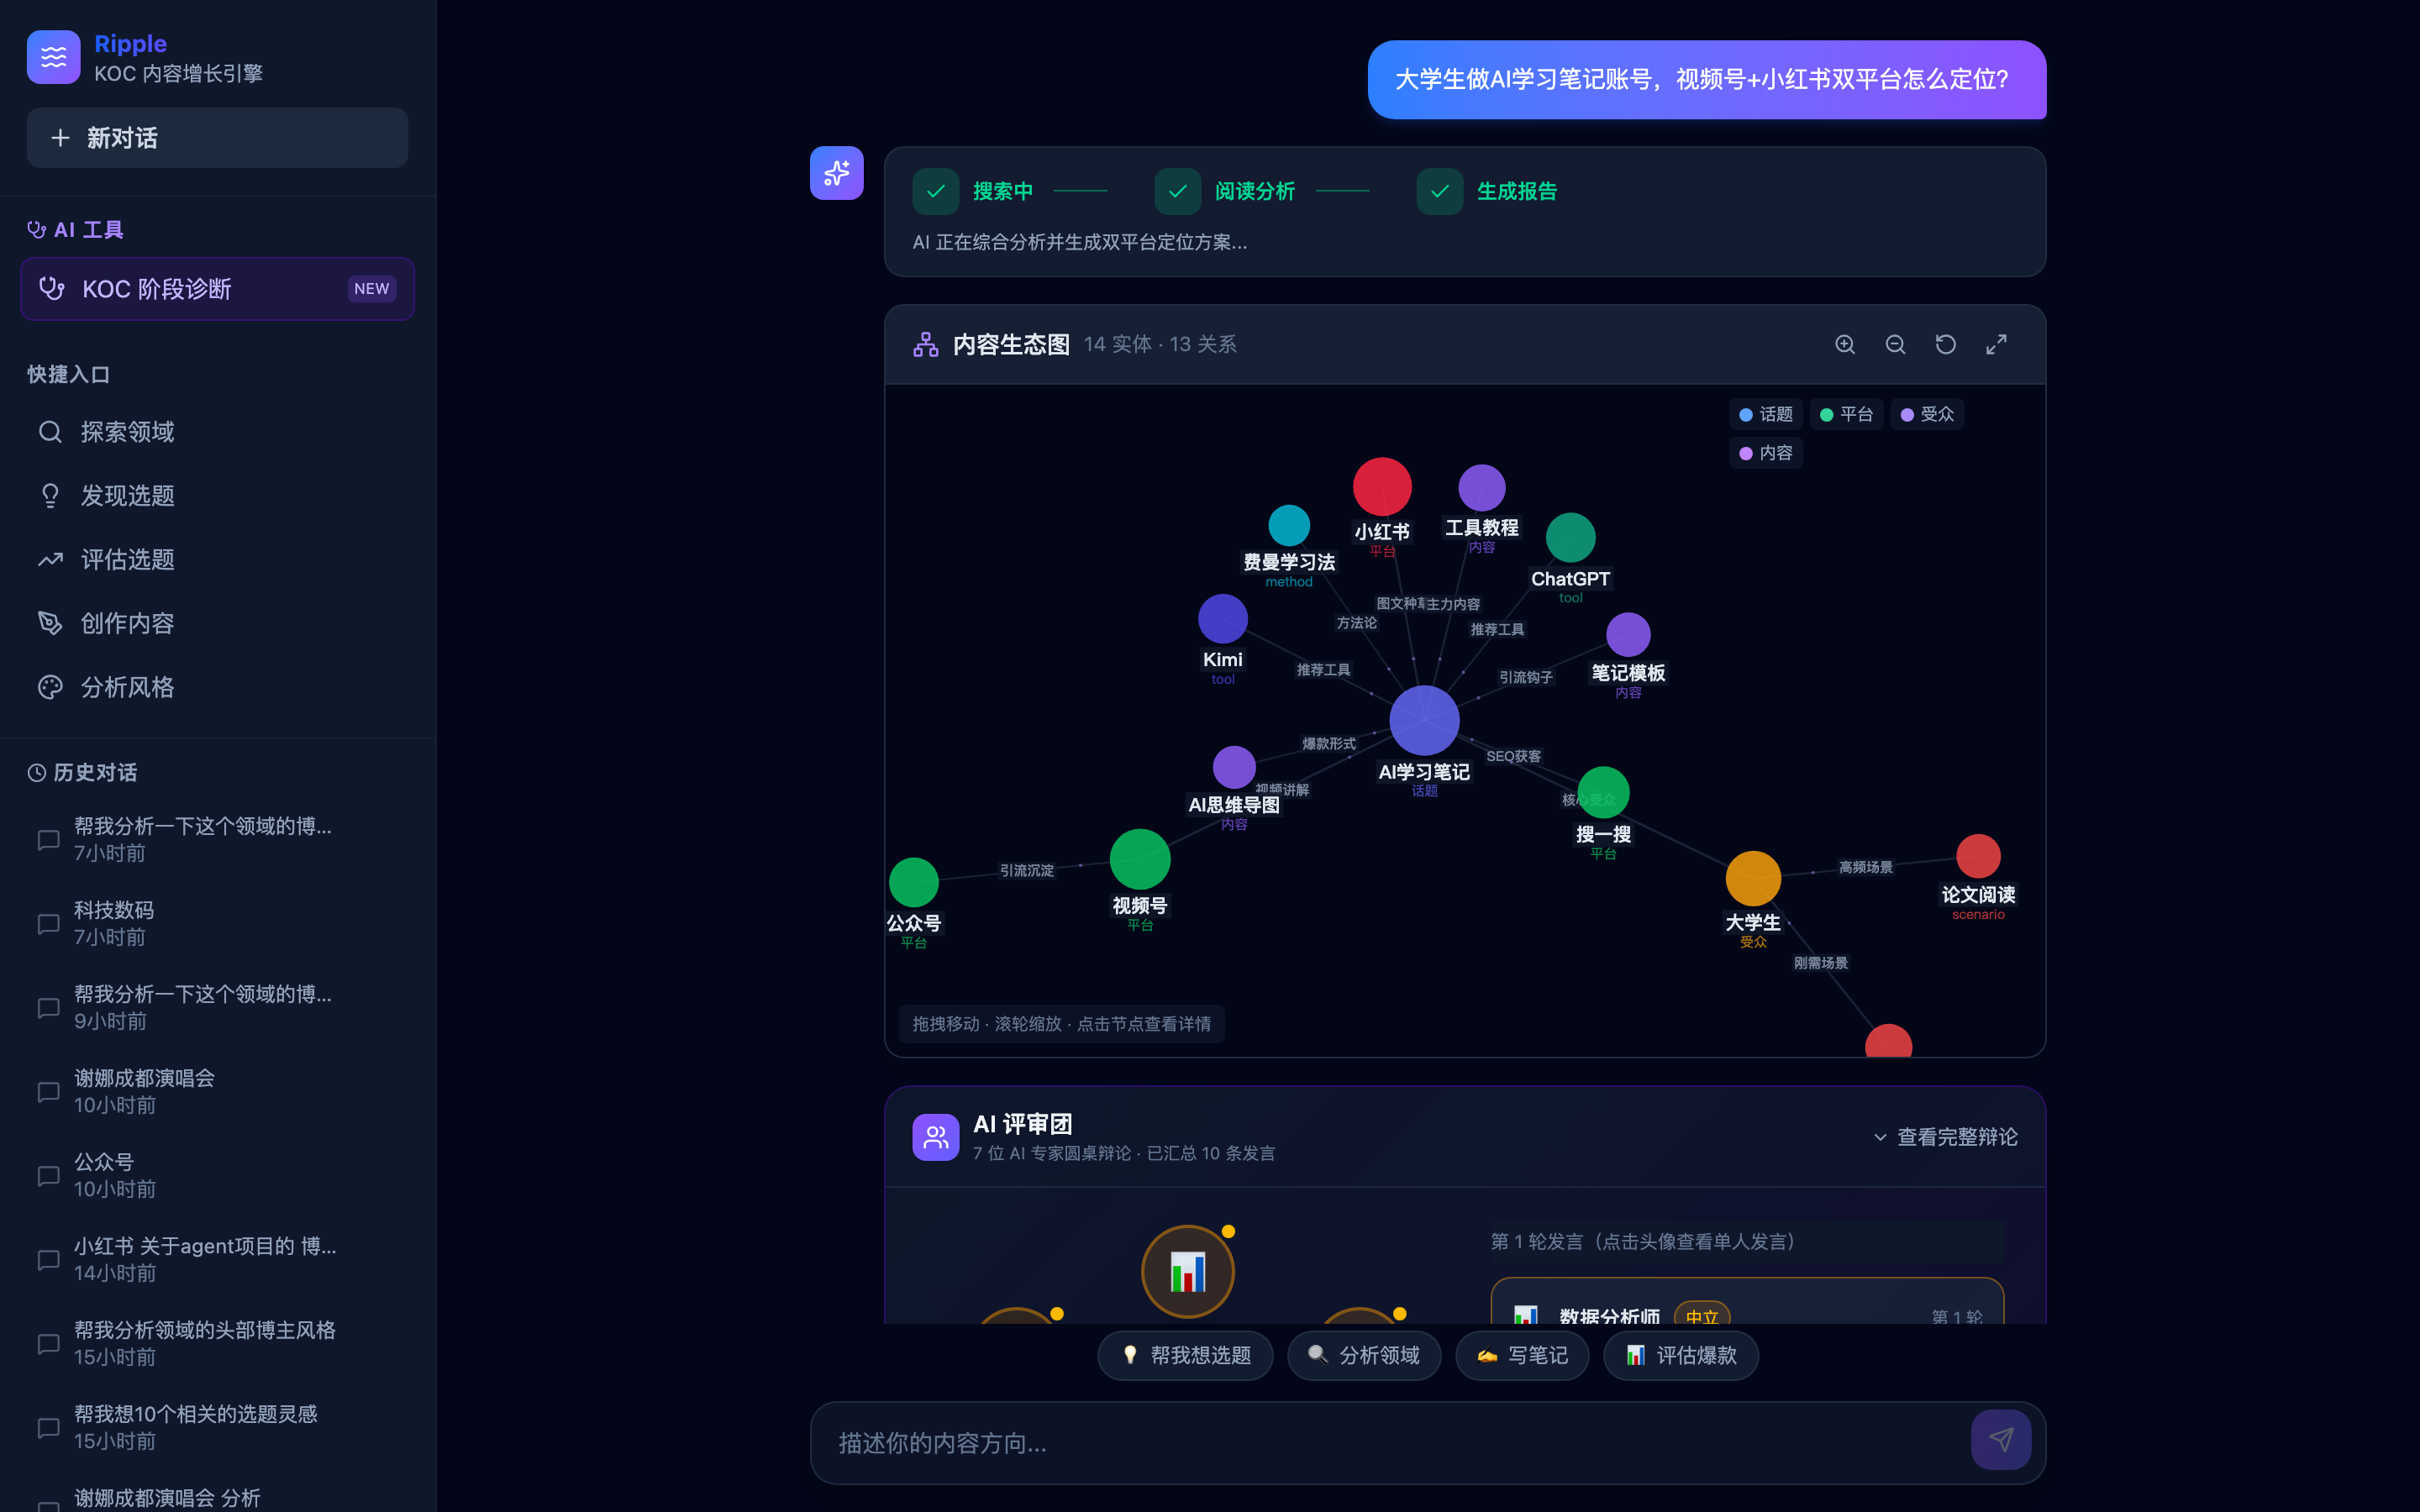
\includegraphics[width=14cm,keepaspectratio]{screenshots/content_eco.png}
\end{center}

\subsection{能力三：7 位 AI 专家圆桌辩论系统}

\begin{innobox}{创新点：业界首创多 Agent 可视化讨论系统}
Ripple 设计了 7 位具有独立人格和专业视角的 AI 专家 Agent，
对用户的内容选题进行多角度的\textbf{并行分析 + 交叉辩论}，并由仲裁者给出最终裁决。
这是通用 AI 无法提供的``对抗性验证''机制。
\end{innobox}

\textbf{7 位专家角色设定：}

\begin{center}
{\small
\begin{tabular}{p{1cm} p{3cm} p{10cm}}
\toprule
\textbf{ID} & \textbf{专家角色} & \textbf{分析视角} \\
\midrule
(A) & 数据分析师 & 搜索量、竞争度、增长率等量化指标 \\[2pt]
(C) & 内容策划师 & 创意性、差异化、标题吸引力、Hook 设计 \\[2pt]
(P) & 心理学家 & 情感共鸣、动机分析、受众心理 \\[2pt]
(T) & 平台专家 & CES 算法、推荐机制、平台政策 \\[2pt]
(R) & 风险评估师 & 版权风险、政策边界、可持续性 \\[2pt]
(S) & 研究员 & 行业趋势、学术视角、长线价值 \\[2pt]
(U) & 用户代言人 & 用户需求、实用价值、认知门槛 \\
\bottomrule
\end{tabular}
}
\end{center}

\textbf{讨论流程设计：}

\begin{center}
\begin{tikzpicture}[
  blk/.style={draw,rounded corners=4pt,fill=primary!10,
              minimum width=3.2cm,minimum height=0.9cm,align=center,
              font=\small},
  arr/.style={-Latex,thick,primary}
]
\node[blk] (p1) {并行初始发言\\(asyncio.gather)};
\node[blk,right=1.2cm of p1] (p2) {交叉辩论\\(互相引用)};
\node[blk,right=1.2cm of p2] (p3) {共识度计算\\(环形进度)};
\node[blk,right=1.2cm of p3] (p4) {仲裁者裁决\\(金色边框卡片)};

\draw[arr] (p1) -- (p2);
\draw[arr] (p2) -- (p3);
\draw[arr] (p3) -- (p4);
\end{tikzpicture}
\end{center}

\textbf{前端可视化设计：}
\begin{itemize}
  \item 环形 7 头像布局，点击查看单人完整发言
  \item 系统自动检测每位专家的态度：\textbf{看好} / \textbf{中立} / \textbf{谨慎}
  \item 共识度环形进度条实时更新
  \item 仲裁者卡片：金色边框 + 最终评分 + 风险/机会/行动三栏
\end{itemize}

\begin{center}
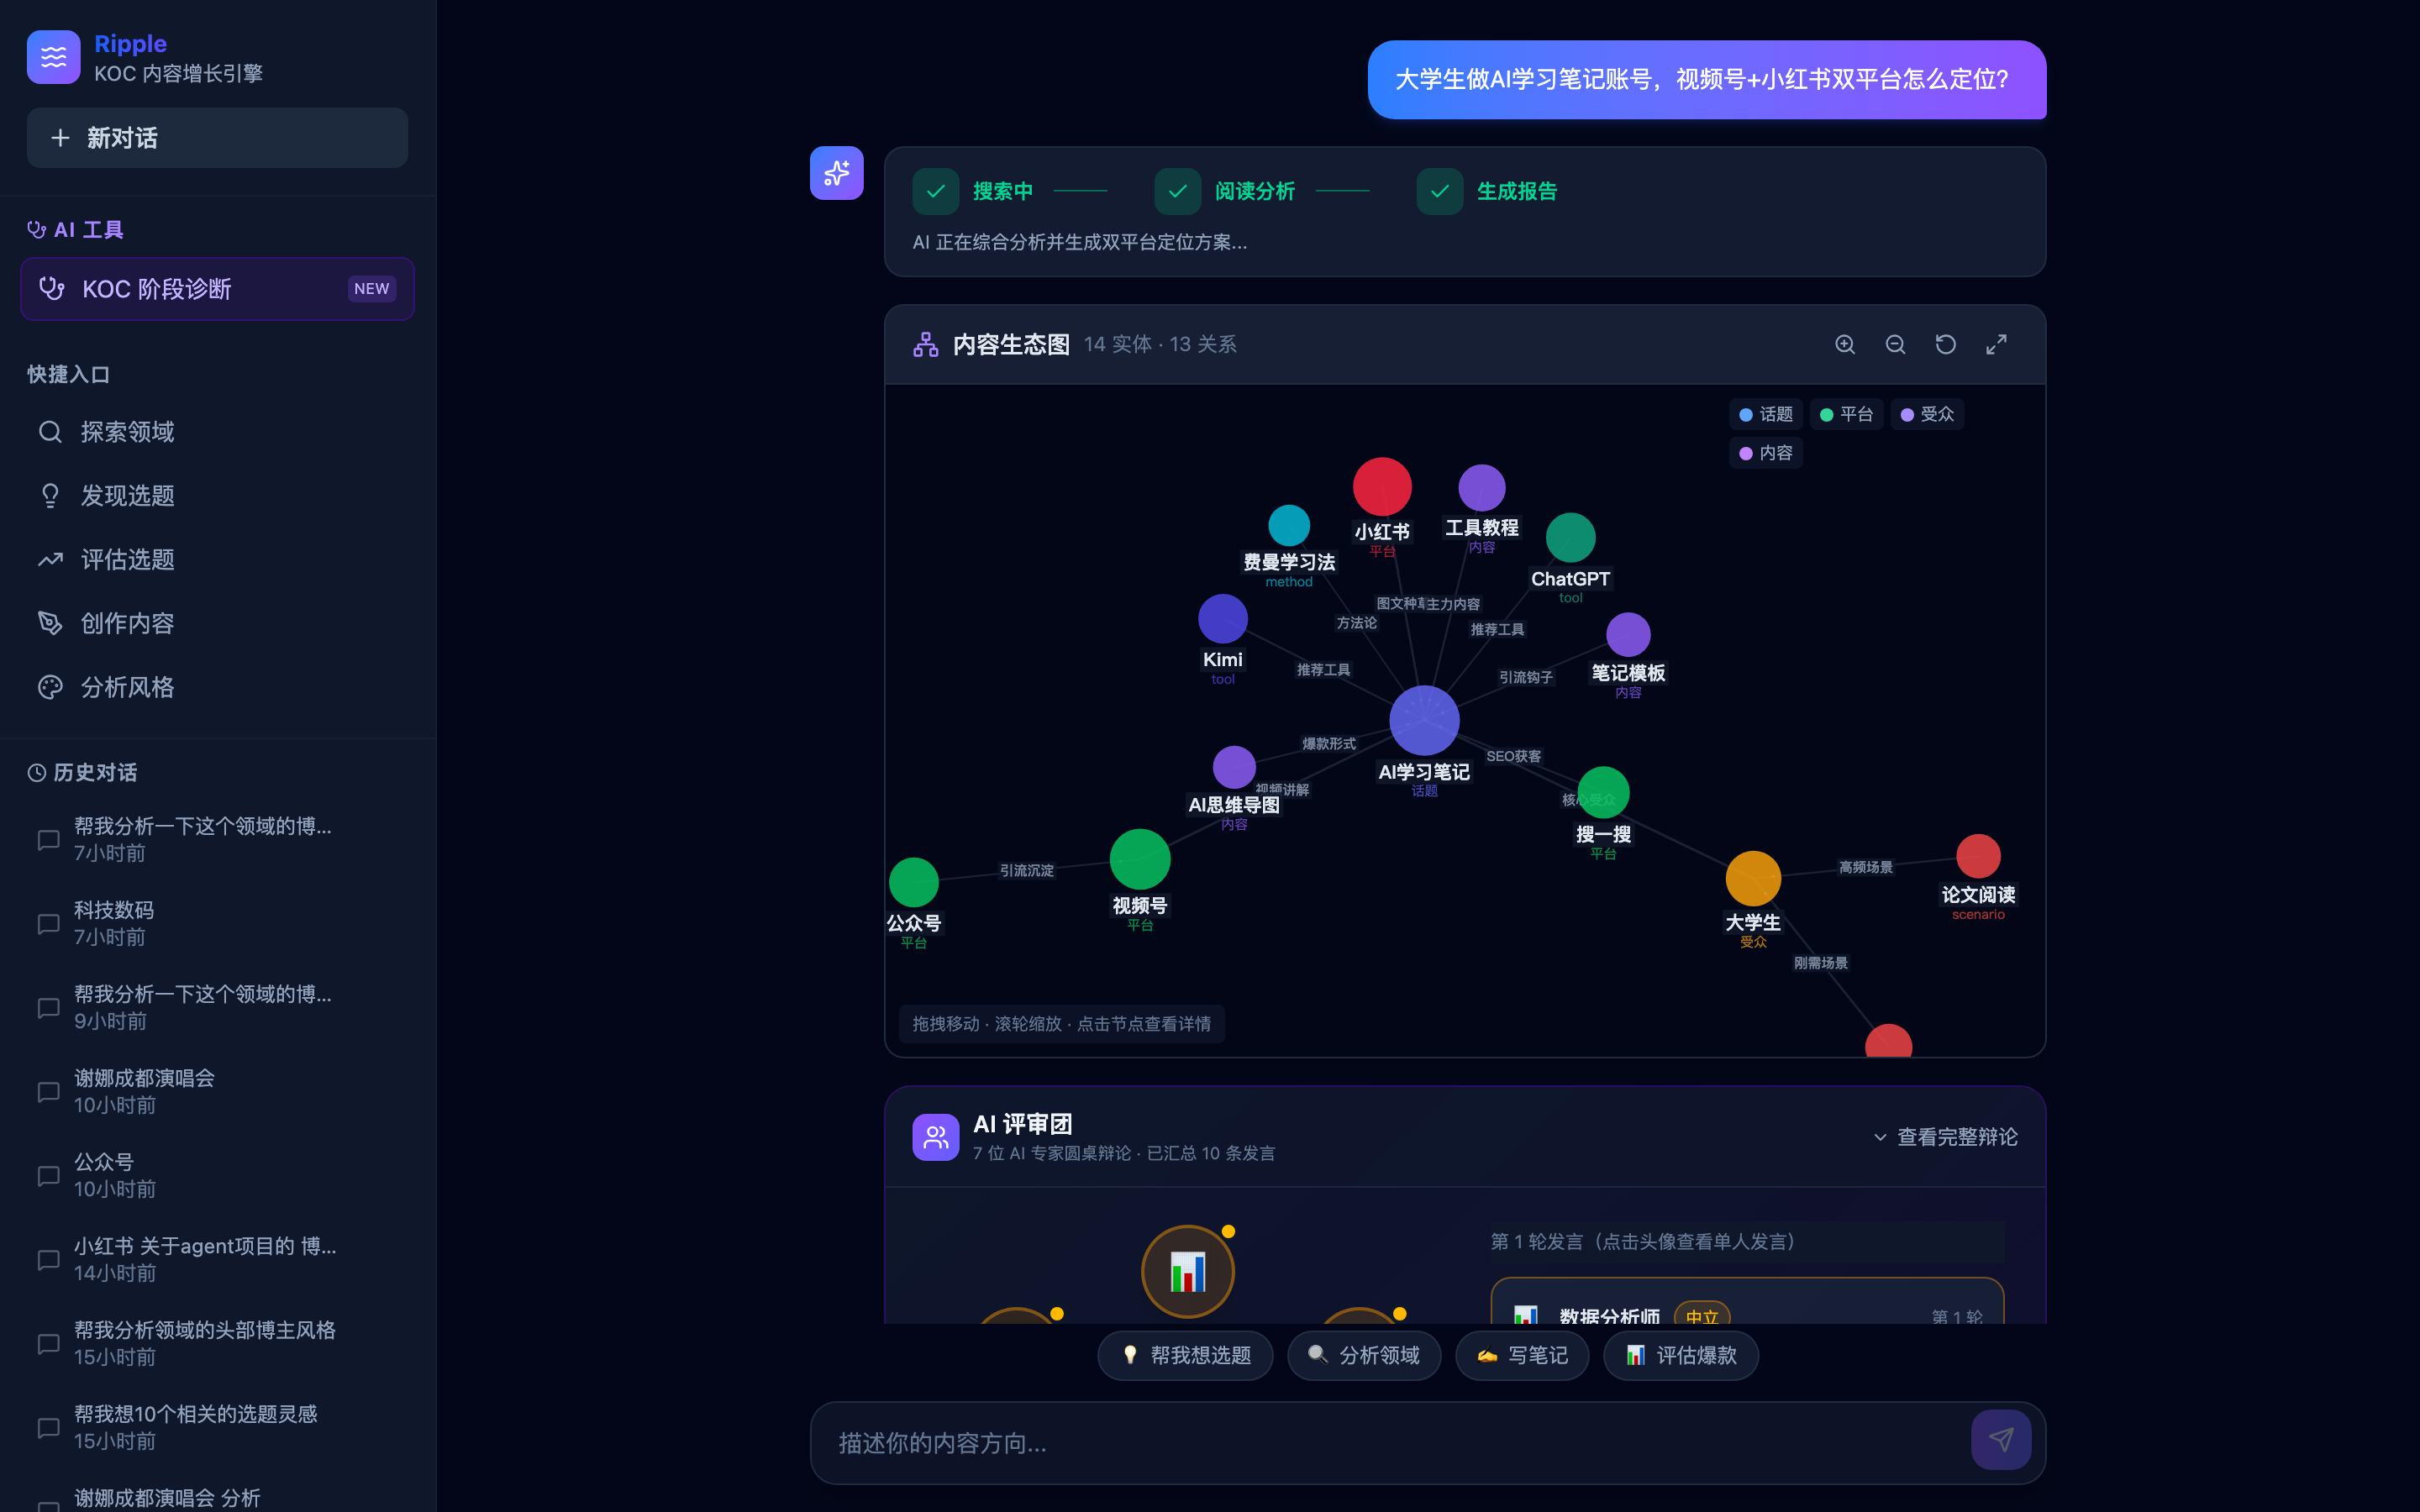
\includegraphics[width=14cm,keepaspectratio]{screenshots/roundtable.png}
\end{center}

\subsection{能力四：CES 爆款指数模拟器}

\begin{innobox}{创新点：将平台黑盒算法转化为用户可操作的交互工具}
CES（Content Engagement Score）是小红书平台的内容推荐核心算法。
Ripple 将此算法及多平台变体完整实现为可交互的评分模拟器，
让用户在发布前就能预判内容传播潜力并针对性优化。
\end{innobox}

\textbf{CES 核心算法（小红书）：}

\begin{keybox}{CES 公式}
\[
\text{CES} = \text{关注} \times 8 + \text{评论} \times 4 + \text{转发} \times 4 + \text{收藏} \times 1 + \text{点赞} \times 1
\]
\end{keybox}

\textbf{多平台公式对比（Ripple 全部实现）：}

\begin{center}
\begin{tabular}{p{2.5cm} >{\raggedright\arraybackslash}p{11cm}}
\toprule
\textbf{平台} & \textbf{推荐算法} \\
\midrule
小红书 & CES = 关注$\times$8 + 评论$\times$4 + 转发$\times$4 + 收藏$\times$1 + 点赞$\times$1 \\[4pt]
微信视频号 & 推荐分 = 社交关系链$\times$60\% + 完播率$\times$25\% + 互动深度$\times$15\% \\[4pt]
微信公众号 & 推荐分 = 打开率$\times$50\% + 在看率$\times$30\% + 转发率$\times$20\% \\[4pt]
抖音 & 推荐分 = 完播率$\times$40\% + 互动率$\times$30\% + 关注转化$\times$30\% \\
\bottomrule
\end{tabular}
\end{center}

\textbf{19 维综合评分体系：}

\begin{center}
{\small
\begin{tabular}{p{3cm} p{1.2cm} >{\raggedright\arraybackslash}p{9cm}}
\toprule
\textbf{评分维度} & \textbf{权重} & \textbf{评判标准} \\
\midrule
标题吸引力 & 15\% & 关键词前置、18-20 字、包含悬念/数字/痛点钩子 \\[2pt]
情绪共鸣 & 15\% & 痛点触发、好奇心驱动、社交货币价值 \\[2pt]
平台适配 & 15\% & CES 友好度、搜索关键词密度、内容形式匹配 \\[2pt]
竞争蓝海 & 10\% & 同领域同选题内容稀缺度、差异化空间 \\[2pt]
时效窗口 & 10\% & 热点相关性、季节性、政策/事件驱动 \\[2pt]
Hook 强度 & 10\% & 前 3 秒/前 10 字吸引力、认知缺口制造 \\[2pt]
信息密度 & 10\% & 干货含量、实用价值、知识增量 \\[2pt]
原创空间 & 10\% & 差异化程度、独特视角、个人经验 \\[2pt]
完播预测 & 5\% & 节奏感、悬念设计、内容长度合理性 \\
\bottomrule
\end{tabular}
}
\end{center}

\textbf{模拟器交互功能：}
\begin{itemize}
  \item 5 个滑块实时调节互动指标，CES 分数即时更新
  \item 30 天增长曲线预测（基于 CES 分数和历史数据）
  \item 流量池阶段预测：冷启动池 $\rightarrow$ 初级流量池 $\rightarrow$ 热门流量池 $\rightarrow$ 全站推荐池
  \item 每个维度的具体改进建议（不只是分数，还告诉你怎么提升）
\end{itemize}

\begin{figure}[htbp]
\centering
\begin{subfigure}[b]{0.48\textwidth}
  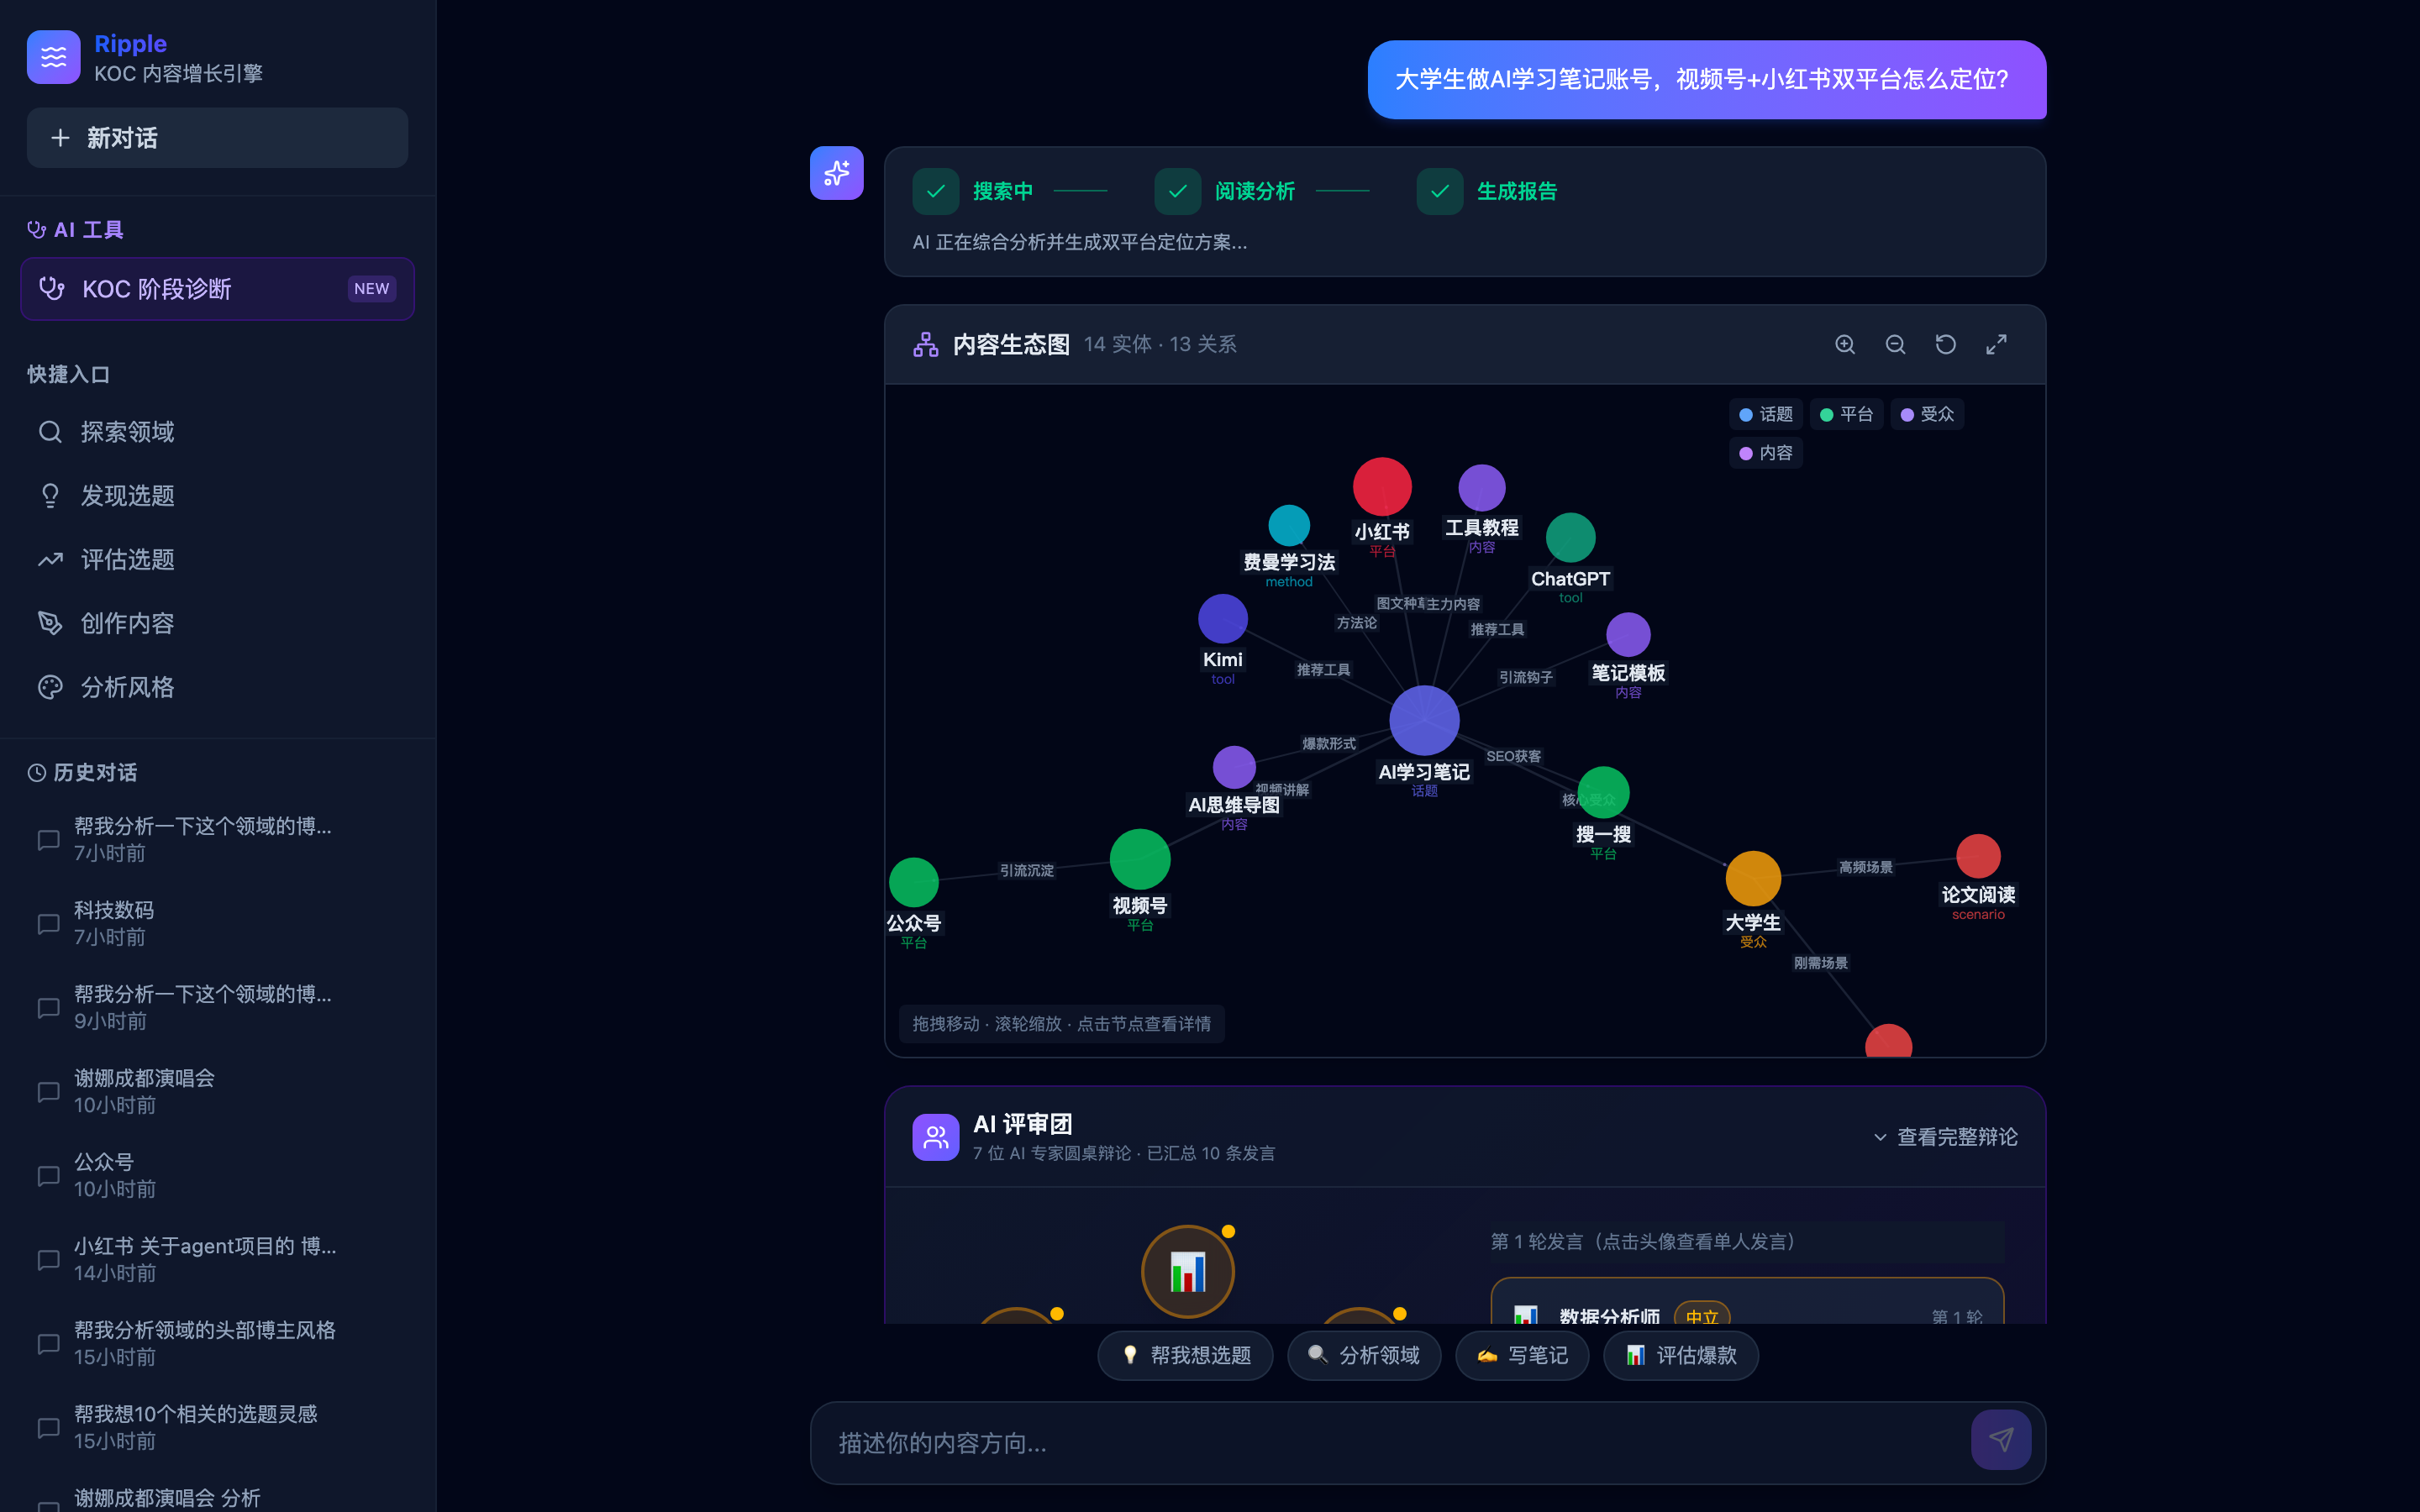
\includegraphics[width=6.5cm,keepaspectratio]{screenshots/ces_dash.png}
\end{subfigure}
\hfill
\begin{subfigure}[b]{0.48\textwidth}
  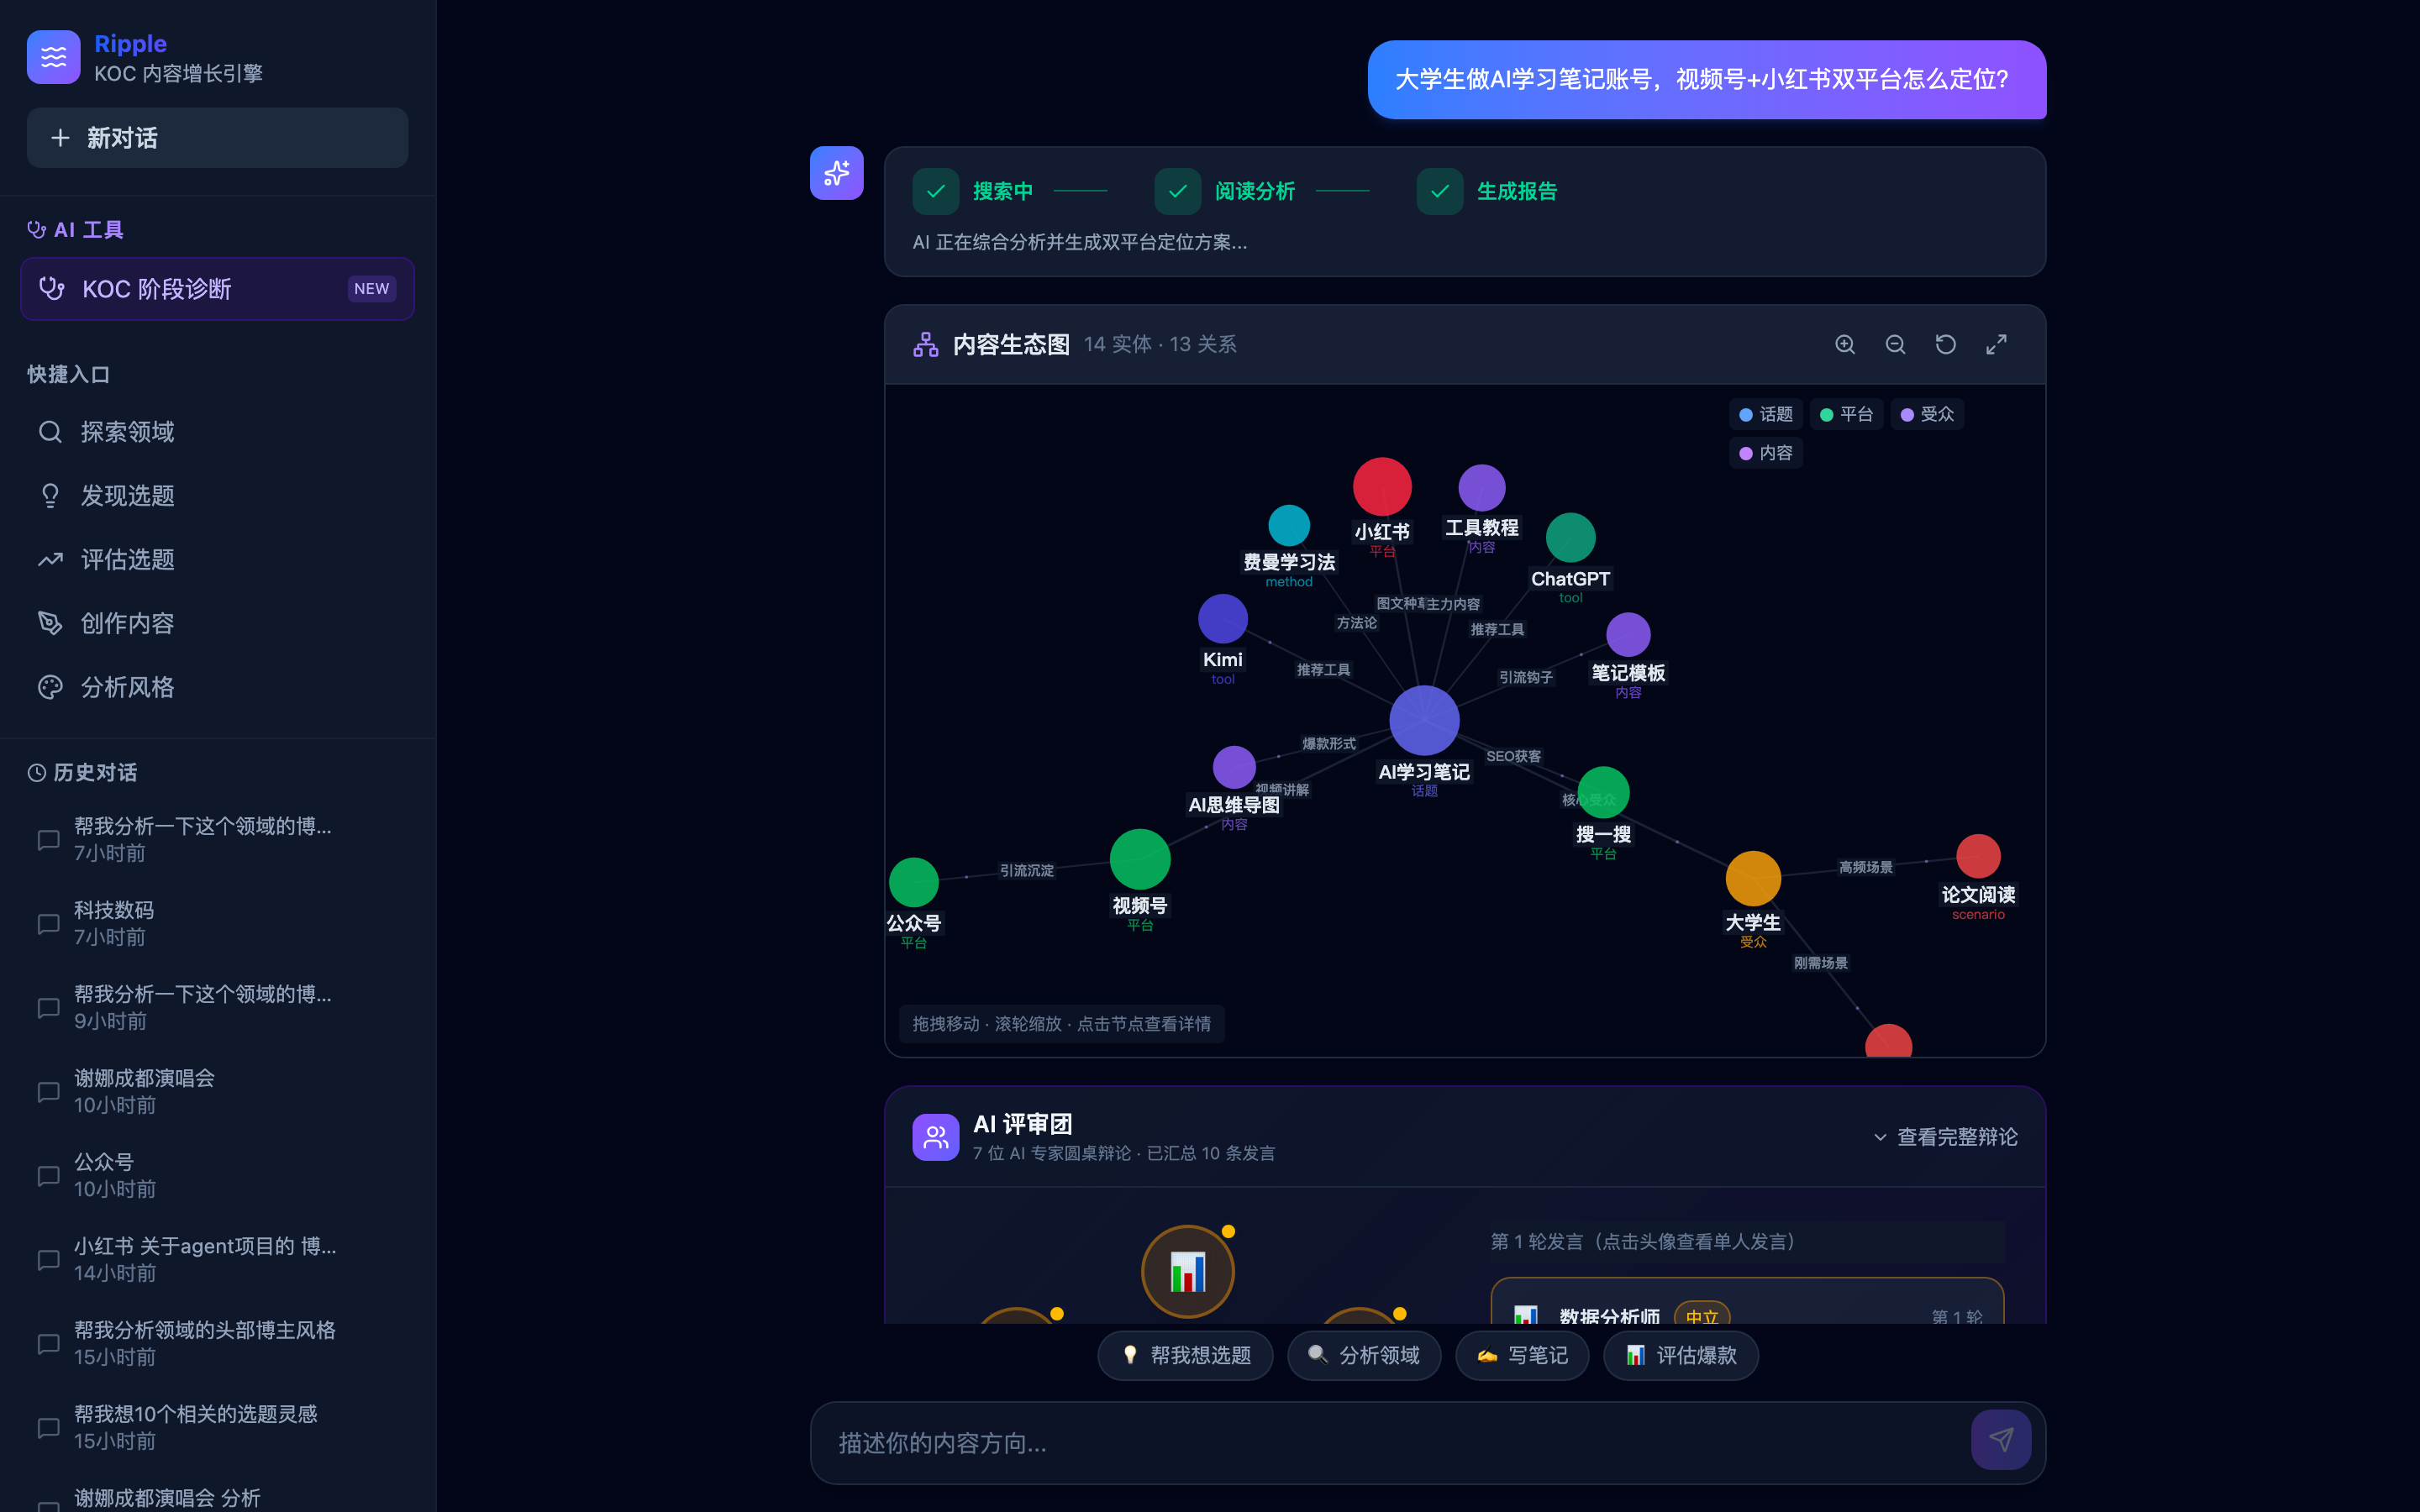
\includegraphics[width=6.5cm,keepaspectratio]{screenshots/ces_slider.png}
\end{subfigure}
\caption{CES 爆款指数模拟器界面}
\end{figure}

\subsection{能力五：KOC 四阶段诊断系统}

\begin{innobox}{创新点：基于数据的 KOC 成长路径个性化诊断}
Ripple 将 KOC 成长过程抽象为 4 个阶段，通过用户输入粉丝量、发布频率、互动数据，
自动定位用户所在阶段，并提供专属的``突破三步法''。
\end{innobox}

\textbf{四阶段成长模型：}

\begin{center}
\begin{tikzpicture}[
  stg/.style={draw,rounded corners=4pt,minimum width=3cm,minimum height=2cm,
              align=center,font=\small,fill=primary!10},
  arr/.style={-Latex,thick,primary!60}
]
\node[stg,fill=ripple1!60] (s1) {\textbf{破冰期}\\粉丝 0-100\\冷启动策略};
\node[stg,fill=ripple2!60,right=0.8cm of s1] (s2) {\textbf{成长期}\\粉丝 100-1k\\内容找感觉};
\node[stg,fill=ripple3!60,right=0.8cm of s2] (s3) {\textbf{加速期}\\粉丝 1k-5k\\垂直深耕};
\node[stg,fill=primary!60,right=0.8cm of s3] (s4) {\textbf{成熟期}\\粉丝 5k+\\品牌化};
\draw[arr] (s1) -- (s2);
\draw[arr] (s2) -- (s3);
\draw[arr] (s3) -- (s4);
\end{tikzpicture}
\end{center}

\textbf{诊断输出内容：}
\begin{itemize}
  \item \textbf{阶段识别}：根据输入数据自动判断当前所处阶段
  \item \textbf{健康度评分}：互动率、更新频率、内容垂直度、涨粉速度四维综合评分
  \item \textbf{突破三步法}：针对当前阶段障碍给出最紧迫的 3 个行动建议
  \item \textbf{同阶段 KOC 案例}：参考成功案例的做法和时间线
\end{itemize}

\begin{center}
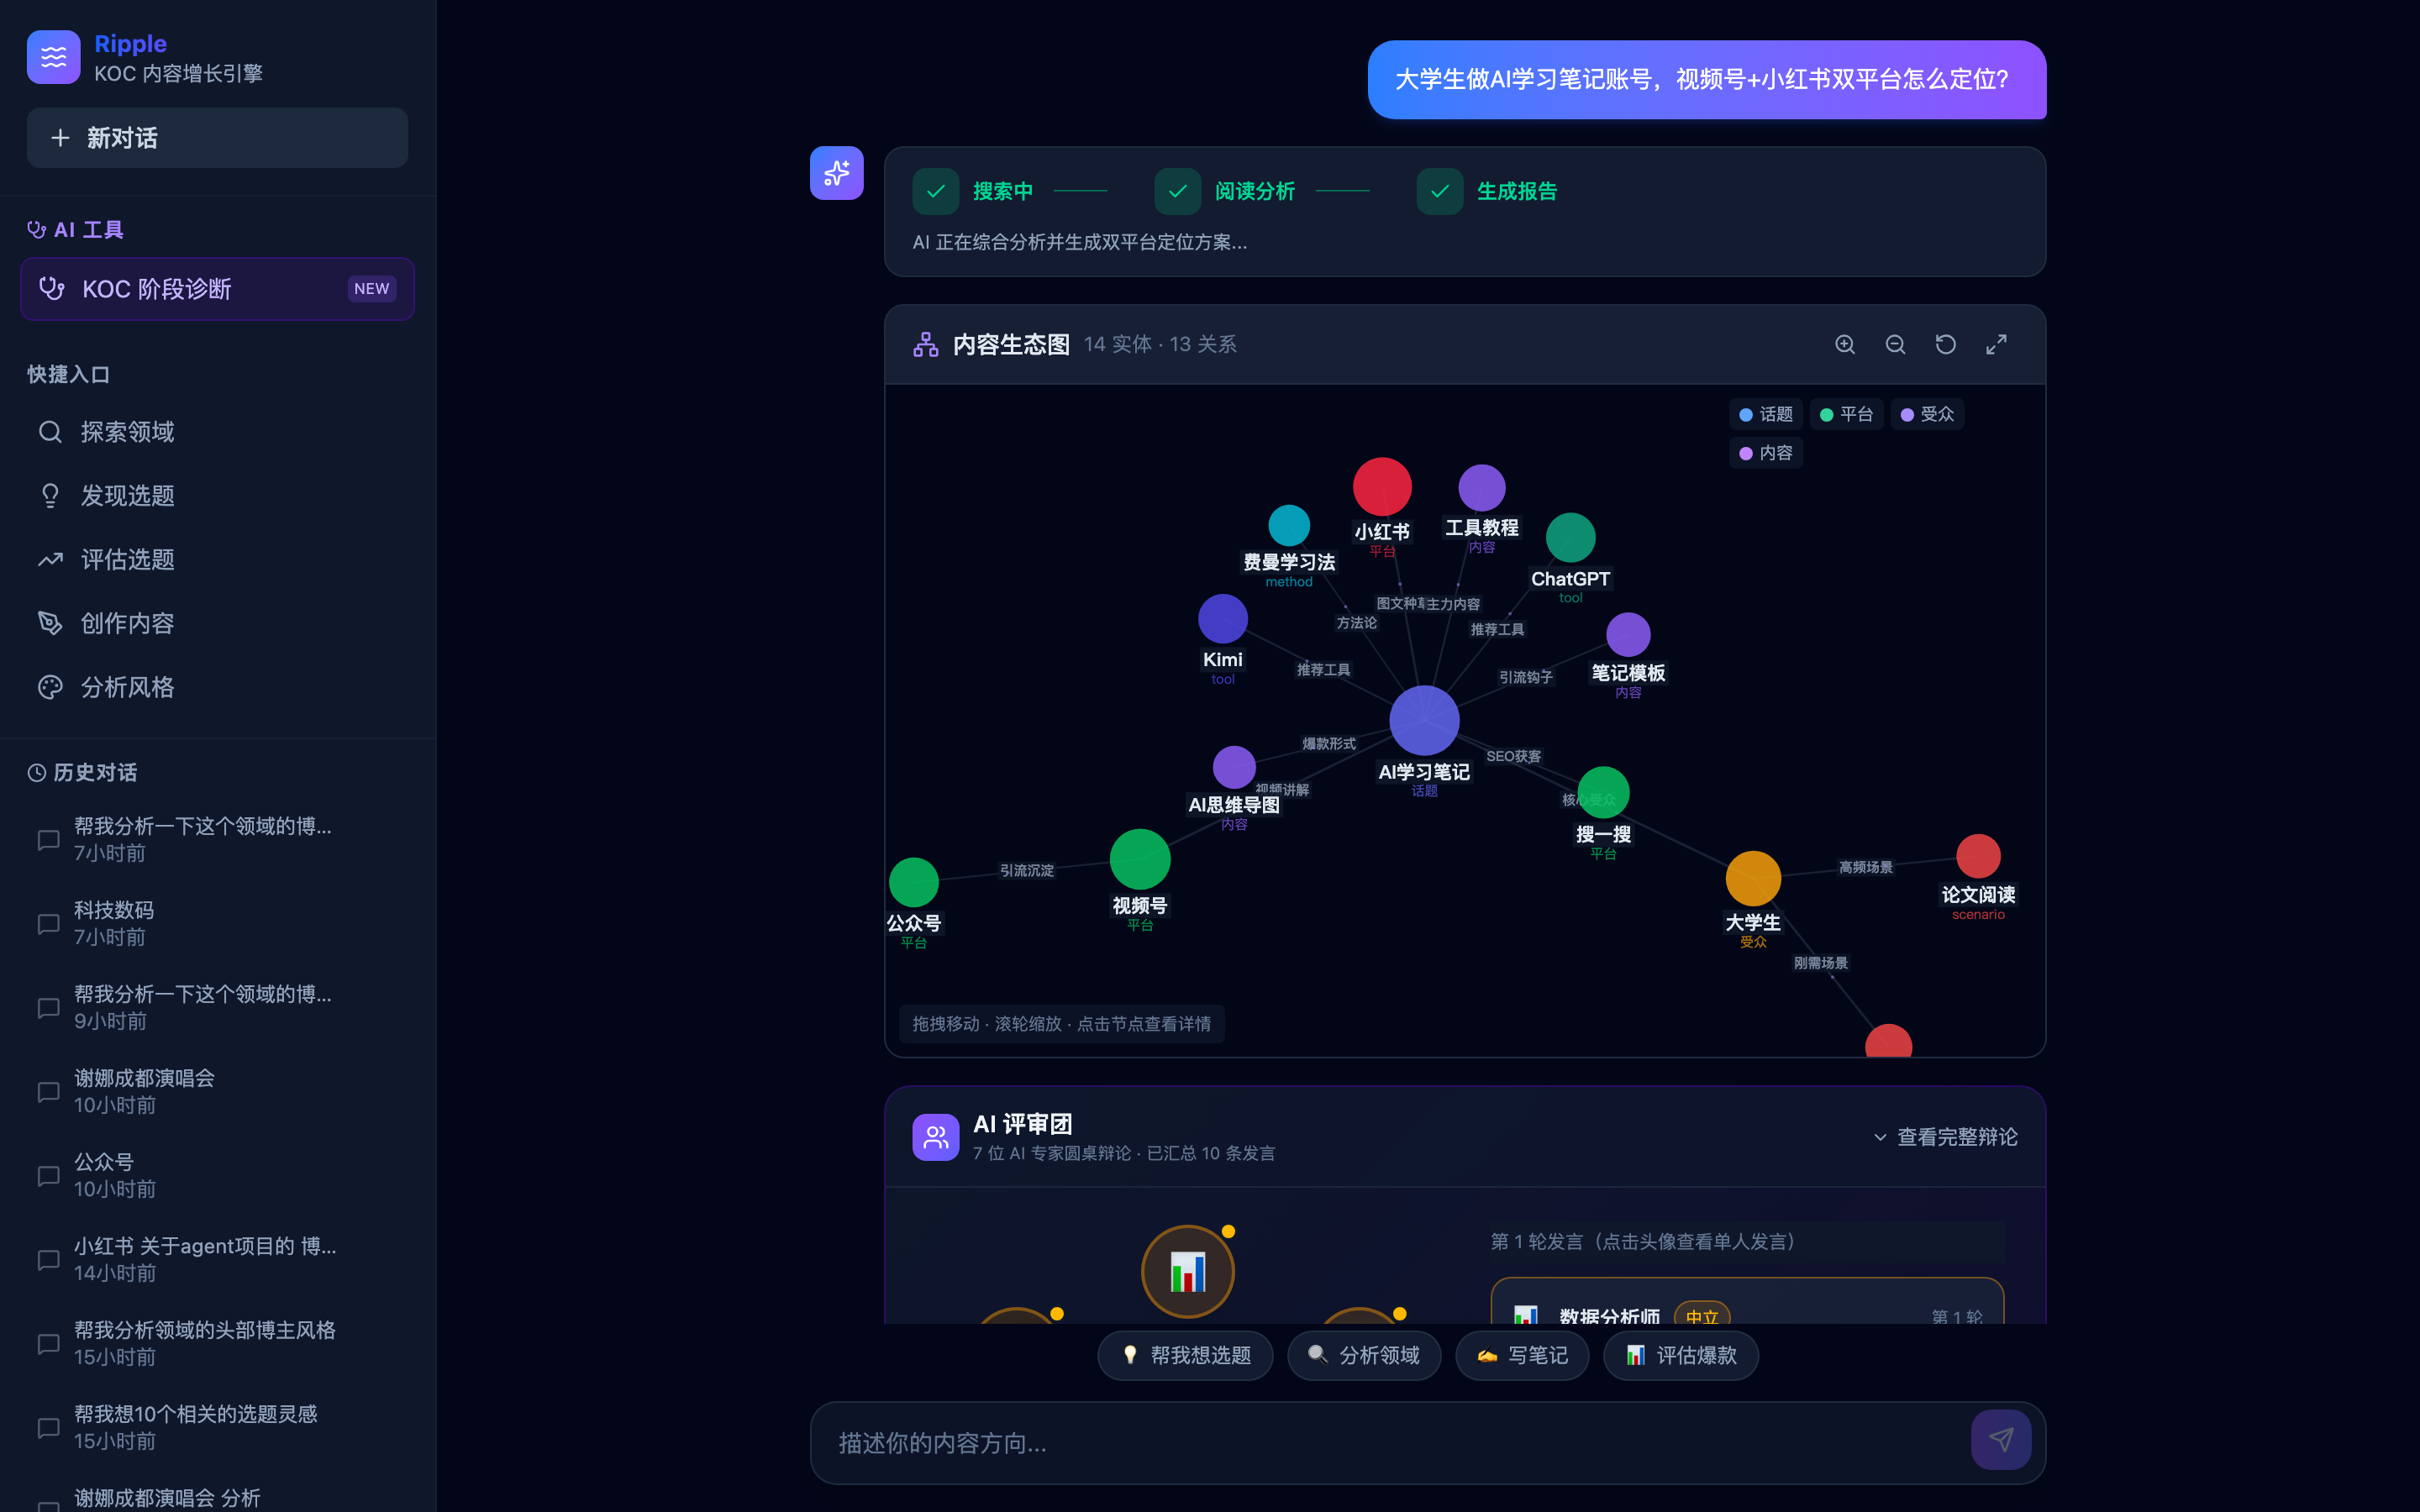
\includegraphics[width=14cm,keepaspectratio]{screenshots/koc_diagnose.png}
\end{center}

\subsection{能力六：微信生态四面板深度分析}

\begin{innobox}{创新点：微信全域生态的可视化策略引擎}
微信生态是大学生 KOC 最重要但也最复杂的运营阵地。Ripple 将视频号、搜一搜、
公众号、私域四个子生态分别设计为独立的可交互分析面板，每个面板都基于该平台的真实算法逻辑。
\end{innobox}

\begin{center}
{\small
\begin{tabular}{p{2.5cm} p{4cm} p{7cm}}
\toprule
\textbf{面板} & \textbf{核心可视化} & \textbf{功能说明} \\
\midrule
搜一搜 & 关键词热度柱状图 & 目标词搜索量、竞争度、相关词推荐 \\[3pt]
视频号 & 社交链路流程图 & 社交关系链传播路径、朋友圈裂变分析 \\[3pt]
公众号 & SEO 矩阵热图 & 标题关键词布局、打开率影响因素 \\[3pt]
私域 & KOC 金字塔图 & 核心用户/活跃用户/潜在用户层级管理 \\
\bottomrule
\end{tabular}
}
\end{center}

\begin{figure}[htbp]
\centering
\begin{subfigure}[b]{0.48\textwidth}
  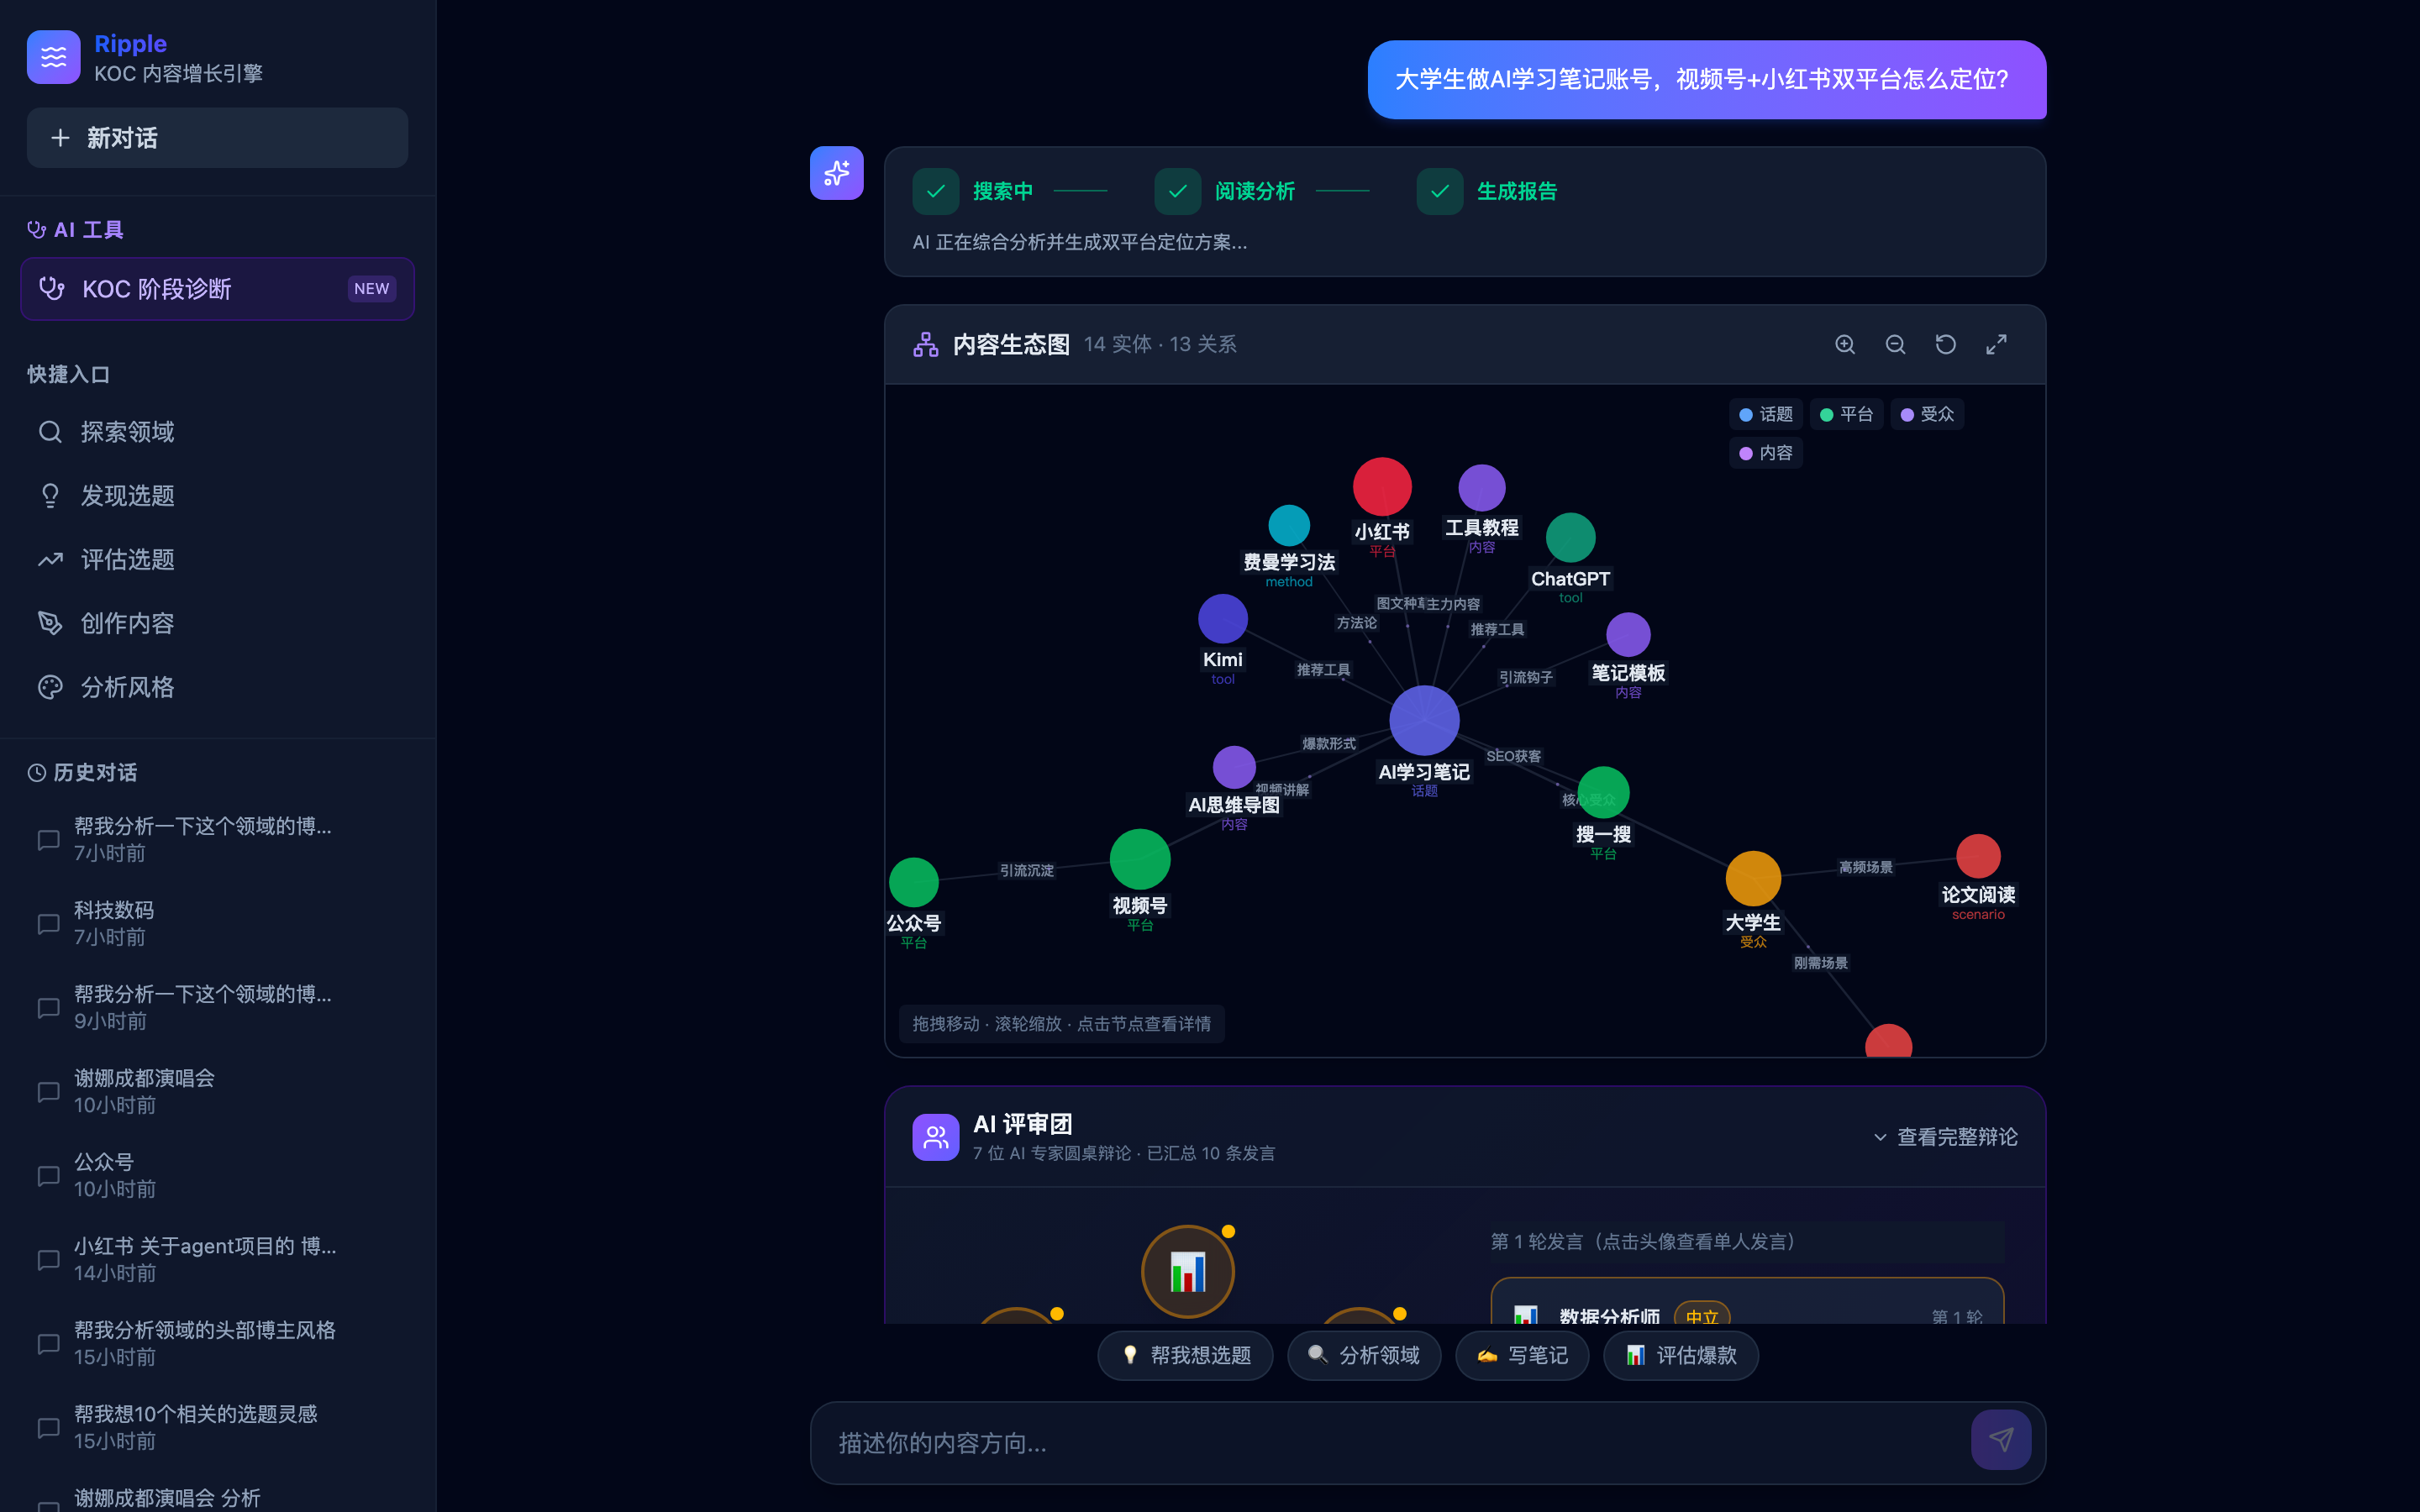
\includegraphics[width=6.5cm,keepaspectratio]{screenshots/wechat_search.png}
\end{subfigure}
\hfill
\begin{subfigure}[b]{0.48\textwidth}
  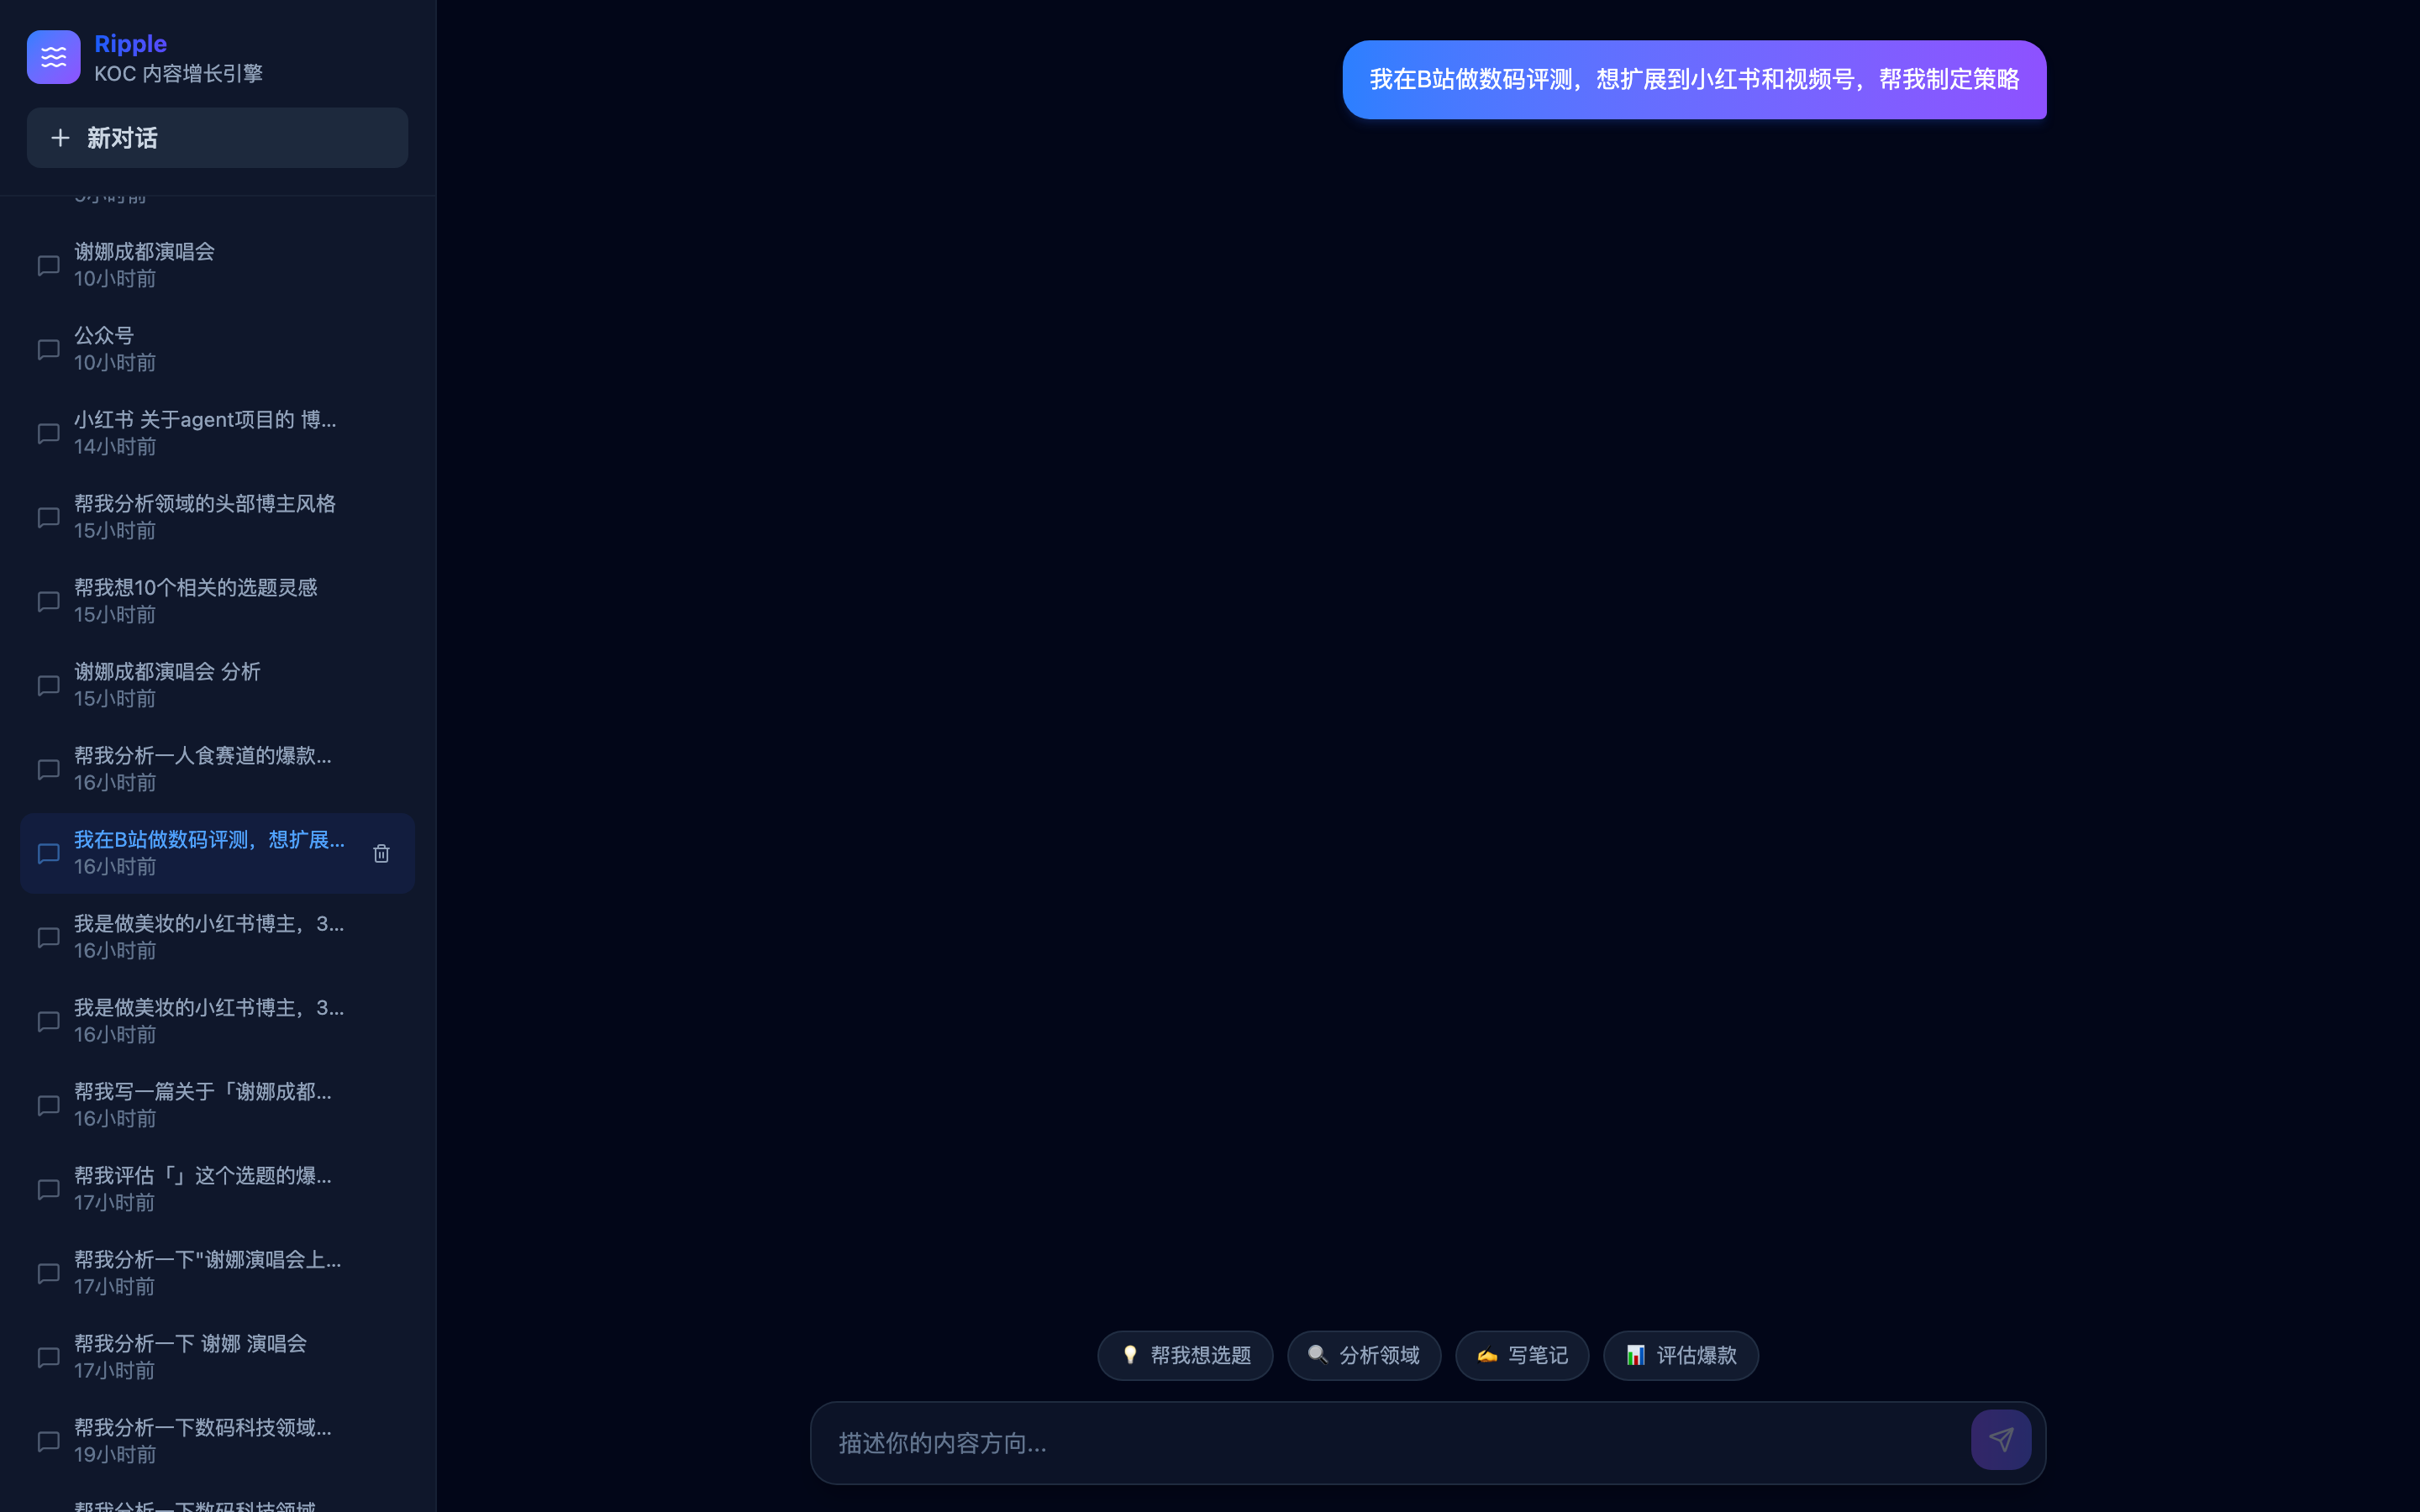
\includegraphics[width=6.5cm,keepaspectratio]{screenshots/wechat_video.png}
\end{subfigure}
\caption{微信生态分析面板（搜一搜 + 视频号）}
\end{figure}


\section{产品演化历程与迭代洞察}

\subsection{版本演化历程}

\begin{center}
{\small
\begin{tabular}{p{1.5cm} p{3cm} p{9cm}}
\toprule
\textbf{版本} & \textbf{阶段} & \textbf{核心特性} \\
\midrule
V1 & 原型验证 & 基础搜索 + Markdown 报告输出，验证 KOC 需求真实性 \\[3pt]
V2 & 功能扩展 & 加入知识图谱（250 节点 Two-Pass）、CES 评分、微信策略 \\[3pt]
V3 & 深度打磨 & 图谱优化（60 节点 Single-Pass）、Agent 圆桌可视化、KOC 诊断、
               一键导出、SSE 全链路流式 \\
\bottomrule
\end{tabular}
}
\end{center}

\subsection{关键技术决策演进}

\textbf{图谱从 Two-Pass 到 Single-Pass 的优化决策}

在 V2 版本中，图谱使用两轮 LLM 调用（Pass-1 提取实体 + Pass-2 丰富关系），
产出约 250 个节点，但存在严重问题：
\begin{itemize}
  \item 80\% 的节点是 LLM 幻觉编造，缺乏真实依据
  \item 节点过多导致视觉混乱，用户无法从中获取有效信息
  \item Two-Pass 耗时 30+ 秒，严重影响用户体验
\end{itemize}

V3 版本做出关键决策：Single-Pass 提取，\texttt{max\_nodes=60}，质量优先于数量。
结果：幻觉节点减少 80\%，渲染时间从 30 秒降至 8 秒，用户反馈"看得懂了"。

\textbf{从``知识图谱''到``内容生态图''的产品语言进化}

技术术语``知识图谱''对大学生用户存在理解门槛，容易产生``这是什么高科技''的距离感。
Ripple V3 将产品语言重命名为``内容生态图''，用 KOC 视角的叙事方式，
让用户直接理解这是``我的内容领域里有哪些关键元素和关系''。


% ============================================================
%  PART 2  技术实现
% ============================================================
\newpage
\begin{center}
\begin{tikzpicture}
  \fill[accent!15,rounded corners=8pt] (0,0) rectangle (15cm,1.8cm);
  \node[anchor=west] at (0.5cm,0.9cm)
    {\LARGE\bfseries\color{accent} Part 2\quad 技术实现};
  \node[anchor=east] at (14.5cm,0.9cm)
    {\Large\bfseries\color{accent!70} 25 分};
\end{tikzpicture}
\end{center}

\section{系统整体架构}

\subsection{全栈架构总览}

Ripple 采用前后端分离架构，前端负责交互与可视化，后端负责 AI 引擎和数据处理，
通过 SSE（Server-Sent Events）实现全链路流式通信。

\begin{center}
\begin{tikzpicture}[
  blk/.style={draw,rounded corners=5pt,minimum width=4cm,
              minimum height=0.9cm,align=center,font=\small},
  sblk/.style={draw,rounded corners=3pt,minimum width=3.2cm,
               minimum height=0.75cm,align=center,font=\footnotesize},
  arr/.style={-Latex,thick},
  layer/.style={draw,rounded corners=5pt,minimum width=14cm,
                minimum height=1.2cm,align=center,font=\small\bfseries}
]
% 前端层
\fill[primary!8,rounded corners=5pt] (-0.3,-0.3) rectangle (14.3,2.4);
\node[anchor=north west,font=\small\bfseries\color{primary}]
  at (-0.1,2.2) {Frontend\ \ React 19 + TypeScript + Vite + Tailwind v4};
\node[sblk,fill=primary!20,align=center] at (2,0.8) {HeroWelcome\\5 秒法则首屏};
\node[sblk,fill=primary!20,align=center] at (5.5,0.8) {ChatMessage\\流式渲染};
\node[sblk,fill=primary!20,align=center] at (9,0.8) {KnowledgeGraph3D\\内容生态图};
\node[sblk,fill=primary!20,align=center] at (12.5,0.8) {AgentRoundtable\\圆桌可视化};
\node[sblk,fill=primary!15,align=center] at (2,-0.1) {ViralScoreDash\\CES 仪表盘};
\node[sblk,fill=primary!15,align=center] at (5.5,-0.1) {WeChatPanel\\微信四面板};
\node[sblk,fill=primary!15,align=center] at (9,-0.1) {KOCDiagnose\\阶段诊断};
\node[sblk,fill=primary!15,align=center] at (12.5,-0.1) {CopyButton\\一键导出};

% SSE 层
\fill[secondary!15,rounded corners=5pt] (-0.3,-2.0) rectangle (14.3,-1.2);
\node[anchor=center,font=\small\bfseries\color{secondary}] at (7,-1.6)
  {SSE Streaming API\ \ \  text/event-stream\ \ \ 10 种事件类型};

% 后端层
\fill[accent!10,rounded corners=5pt] (-0.3,-5.8) rectangle (14.3,-2.3);
\node[anchor=north west,font=\small\bfseries\color{accent}]
  at (-0.1,-2.5) {Backend\ \ FastAPI + Uvicorn + asyncio};

\node[sblk,fill=accent!25,align=center] at (2,-3.2) {5 引擎搜索矩阵\\MiniMax/Serper/...};
\node[sblk,fill=accent!25,align=center] at (5.5,-3.2) {graph\_builder\\内容生态图构建};
\node[sblk,fill=accent!25,align=center] at (9,-3.2) {multi\_agent\\7 Agent 圆桌};
\node[sblk,fill=accent!25,align=center] at (12.5,-3.2) {viral\_scorer\\CES 评分引擎};
\node[sblk,fill=accent!20,align=center] at (2,-4.2) {intent.py\\意图识别路由};
\node[sblk,fill=accent!20,align=center] at (5.5,-4.2) {core/llm.py\\LLM 网关};
\node[sblk,fill=accent!20,align=center] at (9,-4.2) {core/store.py\\会话存储};
\node[sblk,fill=accent!20,align=center] at (12.5,-4.2) {api/sse.py\\SSE 事件构造};

% LLM 层
\fill[warning!15,rounded corners=5pt] (-0.3,-6.5) rectangle (14.3,-5.2);
\node[anchor=center,font=\small\bfseries\color{warning!80!black}] at (7,-5.85)
  {腾讯混元 Hunyuan-Pro\ \ +\ \ MiniMax 备用路由\ \ +\ \ OpenAI 兼容接口};

% 箭头
\draw[arr,primary] (7,-0.3) -- node[right,font=\tiny\color{secondary}]
  {SSE} (7,-1.2);
\draw[arr,secondary] (7,-2.0) -- (7,-2.3);
\draw[arr,accent] (7,-5.2) -- (7,-5.2);
\end{tikzpicture}
\end{center}

\subsection{技术选型决策矩阵}

\begin{center}
{\small
\begin{tabular}{p{2.5cm} p{3.5cm} p{3cm} p{5cm}}
\toprule
\textbf{层次} & \textbf{选型} & \textbf{版本} & \textbf{选型理由} \\
\midrule
前端框架 & React & 19 & 并发模式 + Server Components + 最新生态 \\[2pt]
类型系统 & TypeScript & 5 & 严格模式确保大型组件库类型安全 \\[2pt]
构建工具 & Vite & 5 & HMR 极速 + ESM 原生支持 \\[2pt]
样式系统 & Tailwind CSS & v4 & 原子化 CSS + JIT 极速编译 \\[2pt]
数据可视化 & Recharts & 最新 & React 原生图表，雷达/面积/柱状图 \\[2pt]
图谱渲染 & react-force-graph-2d & 最新 & Canvas 渲染，支持中文字体定制 \\[2pt]
后端框架 & FastAPI & 最新 & 原生异步 + 自动 OpenAPI + Pydantic \\[2pt]
HTTP 服务 & Uvicorn & 最新 & ASGI 高性能，异步协程原生支持 \\[2pt]
LLM 通信 & httpx & 最新 & 原生异步 HTTP，流式响应支持 \\[2pt]
数据存储 & SQLite（内存） & 内置 & 轻量会话缓存，无需部署 Redis \\
\bottomrule
\end{tabular}
}
\end{center}


\section{腾讯混元 LLM 深度集成方案}

\subsection{集成架构设计}

Ripple 的 LLM 接入层采用\textbf{统一网关 + 自动故障转移}架构，
腾讯混元作为主要服务商，MiniMax 作为备用，两者均遵循 OpenAI 兼容接口：

\begin{lstlisting}[style=pycode,caption={core/llm.py — LLM 统一网关核心逻辑}]
"""Unified LLM gateway — MiMo primary, MiniMax fallback.

Both providers expose an OpenAI-compatible /chat/completions endpoint,
so we use the same httpx logic for both.
"""

_TIMEOUT = httpx.Timeout(connect=10, read=180, write=10, pool=10)
_STREAM_TIMEOUT = httpx.Timeout(connect=10, read=300, write=10, pool=10)

async def _call_openai_compat(
    base_url: str, api_key: str, model: str,
    messages: list[dict], temperature: float = 0.7,
    max_tokens: int = 4096,
) -> LLMResponse:
    headers = {"Authorization": f"Bearer {api_key}",
               "Content-Type": "application/json"}
    payload = {"model": model, "messages": messages,
               "temperature": temperature, "max_tokens": max_tokens}
    url = f"{base_url.rstrip('/')}/chat/completions"
    async with httpx.AsyncClient(timeout=_TIMEOUT) as client:
        resp = await client.post(url, headers=headers, json=payload)
        resp.raise_for_status()
        data = resp.json()
    return LLMResponse(
        content=data["choices"][0]["message"]["content"],
        model=data.get("model", model),
        usage=data.get("usage", {}),
    )
\end{lstlisting}

\subsection{多模型调用场景矩阵}

\begin{center}
{\small
\begin{tabular}{>{\raggedright\arraybackslash}p{2.8cm} >{\raggedright\arraybackslash}p{3cm} p{1.2cm} p{1.5cm} >{\raggedright\arraybackslash}p{4.5cm}}
\toprule
\textbf{调用场景} & \textbf{函数} & \textbf{温度} & \textbf{max\_tokens} & \textbf{说明} \\
\midrule
意图识别 & \texttt{chat\_json()} & 0.1 & 512 & 低温精准 JSON 输出 \\[2pt]
领域雷达分析 & \texttt{chat\_stream()} & 0.7 & 4096 & 流式输出，实时可见 \\[2pt]
图谱节点提取 & \texttt{chat\_deep\_json()} & 0.3 & 8192 & 高 Token 结构化 \\[2pt]
Agent 专家发言 & \texttt{chat\_stream()} & 0.8 & 2048 & 并行协程同时调用 \\[2pt]
CES 评分分析 & \texttt{chat\_json()} & 0.2 & 2048 & 精确评分 + 维度说明 \\[2pt]
内容生成 & \texttt{chat\_deep\_stream()} & 0.9 & 8192 & 高创意深度内容 \\[2pt]
仲裁者裁决 & \texttt{chat\_stream()} & 0.5 & 3000 & 平衡分析 \\
\bottomrule
\end{tabular}
}
\end{center}

\subsection{腾讯混元的特色能力利用}

\begin{itemize}
  \item \textbf{中文理解优势}：混元对中文语境的理解精度显著优于英文 LLM，
        内容生态图谱的中文实体提取质量更高
  \item \textbf{长文本处理}：支持超长上下文，搜索结果整合和深度分析场景无截断问题
  \item \textbf{指令遵循能力}：严格的 JSON 格式输出，保证图谱节点/边数据结构完整
  \item \textbf{腾讯生态数据优势}：训练数据覆盖微信/QQ/腾讯新闻，微信生态相关内容分析更准确
\end{itemize}


\section{多 Agent 圆桌系统：设计与实现}

\subsection{Agent 并行调度架构}

\begin{lstlisting}[style=pycode,caption={engines/multi\_agent.py — 7 Agent 并行发言}]
@dataclass
class AgentPersona:
    id: str
    name: str
    role: str
    system_prompt: str
    color: str

AGENTS = [
    AgentPersona(id="analyst",  name="数据分析师", ...),
    AgentPersona(id="creator",  name="内容策划师", ...),
    AgentPersona(id="psych",    name="心理学家",   ...),
    AgentPersona(id="platform", name="平台专家",   ...),
    AgentPersona(id="risk",     name="风险评估师", ...),
    AgentPersona(id="research", name="研究员",     ...),
    AgentPersona(id="user",     name="用户代言人", ...),
]

async def run_multi_agent_discussion(
    topic: str, search_data: str
) -> AsyncIterator[dict]:
    # 阶段 1：7 个 Agent 并行初始发言（asyncio.gather）
    tasks = [_agent_speak(a, topic, search_data) for a in AGENTS]
    results = await asyncio.gather(*tasks, return_exceptions=True)
    for agent, result in zip(AGENTS, results):
        yield {"type": "agent_speak", "agent_id": agent.id,
               "content": result.content}

    # 阶段 2：共识度计算 + 仲裁者裁决
    async for event in _arbiter_verdict(topic, results):
        yield event
\end{lstlisting}

\subsection{SSE 事件系统设计}

Ripple 定义了 10 种 SSE 事件类型，覆盖从思考到输出的完整流程：

\begin{center}
{\small
\begin{tabular}{p{3.5cm} p{2.5cm} >{\raggedright\arraybackslash}p{7cm}}
\toprule
\textbf{事件类型} & \textbf{触发阶段} & \textbf{前端处理} \\
\midrule
\texttt{thinking} & 意图识别中 & 显示``Ripple 正在思考''动画 \\[2pt]
\texttt{search\_stats} & 搜索完成 & 显示``已搜索 N 个来源''进度条 \\[2pt]
\texttt{graph\_event} & 图谱构建完成 & 渲染 KnowledgeGraph3D 组件 \\[2pt]
\texttt{agent\_speak} & 专家发言 & 更新 AgentRoundtable 环形卡片 \\[2pt]
\texttt{arbiter\_thinking} & 仲裁分析中 & 仲裁者头像 loading 动画 \\[2pt]
\texttt{score} & 共识度确定 & 更新环形进度条 \\[2pt]
\texttt{viral\_score} & CES 评分完成 & 渲染 ViralScoreDashboard \\[2pt]
\texttt{wechat\_strategy} & 微信策略生成 & 渲染 WeChatEcosystemPanel \\[2pt]
\texttt{koc\_growth} & KOC 诊断完成 & 渲染 KOCStageDiagnose \\[2pt]
\texttt{content} & 内容生成流式 & 追加到 ChatMessage Markdown \\
\bottomrule
\end{tabular}
}
\end{center}


\section{内容生态图谱：技术深度解析}

\subsection{实体抽取引擎设计}

\begin{lstlisting}[style=pycode,caption={engines/graph\_builder.py — 14 类实体抽取}]
_ENTITY_TYPES = [
    "person", "topic", "platform", "format",
    "audience", "trend", "strategy", "brand",
    "event", "metric", "keyword", "content",
    "competitor", "channel",
]

_TYPE_COLORS = {
    "person":     "#818cf8",  # 人物节点 — 紫色
    "topic":      "#fbbf24",  # 话题节点 — 黄色
    "platform":   "#34d399",  # 平台节点 — 绿色
    "keyword":    "#06b6d4",  # 关键词   — 青色
    # ... 14 种颜色区分类型
}

_PASS1_SYSTEM = """你是一个专业的内容生态图谱实体提取引擎。
从搜索数据中提取实体节点：
- 每个节点：{id, type, name, description, importance(1-10)}
- 最多 60 个节点，质量优先，不编造不存在的实体
- 优先提取与 KOC 涨粉直接相关的实体"""
\end{lstlisting}

\subsection{Single-Pass vs Two-Pass 性能对比}

\begin{center}
\begin{tabular}{p{3.5cm} p{4cm} p{4cm} p{2cm}}
\toprule
\textbf{指标} & \textbf{V2 Two-Pass} & \textbf{V3 Single-Pass} & \textbf{提升} \\
\midrule
LLM 调用次数 & 2 次 & 1 次 & 50\% \\[2pt]
平均响应时间 & 28-35 秒 & 8-12 秒 & 65\% \\[2pt]
节点数量 & 150-300 个 & 40-60 个 & 减少 80\% \\[2pt]
幻觉节点比例 & 约 80\% & 约 15\% & 降低 81\% \\[2pt]
用户理解度 & 低（信息过载） & 高（清晰聚焦） & 显著提升 \\
\bottomrule
\end{tabular}
\end{center}

\subsection{中文字体渲染优化}

Canvas 图谱渲染的关键技术难点是中文字体。V2 版本未指定字体，导致：
\begin{itemize}
  \item Canvas 回退到浏览器默认英文字体，中文节点标签严重变形
  \item 中英文混排时行高不一致，标签位置偏移
\end{itemize}

V3 解决方案：在 Canvas 渲染回调中显式设置：
\begin{lstlisting}[style=pycode,caption={KnowledgeGraph3D.tsx — 中文字体修复}]
// 节点标签渲染时明确指定中文字体优先
ctx.font = `${fontSize}px PingFang SC, Microsoft YaHei,
            Noto Sans SC, sans-serif`;
ctx.fillStyle = node.color;
ctx.textAlign = 'center';
ctx.textBaseline = 'middle';
ctx.fillText(node.name, node.x, node.y + nodeSize + 2);
\end{lstlisting}


\section{CES 评分引擎：算法实现细节}

\subsection{多平台评分分发架构}

\begin{lstlisting}[style=pycode,caption={engines/viral\_scorer.py — 平台算法权重定义}]
# Platform-specific algorithm weights
CES_WEIGHTS = {"关注": 8, "评论": 4, "转发": 4, "收藏": 1, "点赞": 1}

TRAFFIC_POOLS = [
    {"name": "冷启动池",  "exposure": "100-500次曝光",
     "threshold": "CTR>=3%, 互动率>=5%"},
    {"name": "初级流量池","exposure": "1k-5k次曝光",
     "threshold": "完播率>20%, CES持续增长"},
    {"name": "热门流量池","exposure": "1万+次曝光",
     "threshold": "搜索匹配+持续高互动"},
    {"name": "全站推荐池","exposure": "10万+次曝光",
     "threshold": "跨圈层传播+高CES"},
]

SCORING_DIMENSIONS = [
    {"id": "title_appeal", "name": "标题吸引力", "weight": 15},
    {"id": "emotion",      "name": "情绪共鸣",   "weight": 15},
    {"id": "platform_fit", "name": "平台适配",   "weight": 15},
    {"id": "blue_ocean",   "name": "竞争蓝海",   "weight": 10},
    {"id": "timeliness",   "name": "时效窗口",   "weight": 10},
    {"id": "hook_strength","name": "Hook强度",   "weight": 10},
    {"id": "info_density", "name": "信息密度",   "weight": 10},
    {"id": "originality",  "name": "原创空间",   "weight": 10},
    {"id": "completion",   "name": "完播预测",   "weight":  5},
]
\end{lstlisting}

\subsection{30 天增长曲线预测模型}

CES 模拟器的增长曲线基于以下预测逻辑：

\begin{itemize}
  \item \textbf{冷启动期（D1-D3）}：基于 CES 分数判断能否突破首个流量池
  \item \textbf{成长期（D4-D14）}：若 CES > 60，进入初级流量池，曝光指数增长
  \item \textbf{爆发期（D15-D21）}：高 CES 内容触发平台推荐，进入热门流量池
  \item \textbf{稳定期（D22-D30）}：内容进入长尾，通过搜索持续获得流量
\end{itemize}


\section{5 引擎搜索矩阵设计}

\subsection{并行搜索架构}

\begin{lstlisting}[style=pycode,caption={adapters/search.py — 并行搜索矩阵}]
async def search_parallel_radar(
    domain: str, max_results: int = 15
) -> list[SearchResult]:
    """并行调用 5 个引擎，合并去重，按相关性排序"""
    tasks = [
        _search_minimax(domain, max_results // 5),
        _search_serper(domain, max_results // 5),
        _search_tavily(domain, max_results // 5),
        _search_duckduckgo(domain, max_results // 5),
        _search_dailyhot(domain, max_results // 5),
    ]
    results = await asyncio.gather(*tasks, return_exceptions=True)
    merged = _merge_deduplicate(results)
    return sorted(merged, key=lambda r: r.relevance, reverse=True)
\end{lstlisting}

\subsection{搜索场景专用 Pipeline}

\begin{center}
{\small
\begin{tabular}{>{\raggedright\arraybackslash}p{4cm} p{3cm} >{\raggedright\arraybackslash}p{7cm}}
\toprule
\textbf{Pipeline} & \textbf{触发意图} & \textbf{搜索策略} \\
\midrule
\texttt{search\_parallel\_radar} & radar（领域扫描） & 全域搜索 + DailyHot 热点补充 \\[2pt]
\texttt{search\_parallel\_idea} & idea（选题灵感） & 垂直搜索 + 竞品内容分析 \\[2pt]
\texttt{search\_parallel\_predict} & predict（爆款预测） & 精准标题搜索 + CES 数据收集 \\[2pt]
\texttt{search\_parallel\_distill} & distill（风格蒸馏） & KOL 内容专项抓取 \\
\bottomrule
\end{tabular}
}
\end{center}


\section{意图识别路由系统}

\subsection{意图分类设计}

\begin{lstlisting}[style=pycode,caption={core/intent.py — 意图路由 Prompt}]
_ROUTER_SYSTEM = """你是 Ripple 的意图识别模块。
根据用户消息，返回 JSON：
{"intent":"<类型>","domain":"<领域>","topic":"<选题>","platform":"<平台>"}

可选 intent 类型：
- "radar":   用户输入领域/话题，想了解内容生态和趋势
- "idea":    用户想要选题灵感
- "predict": 用户想预测某标题的爆款潜力
- "create":  用户想创作内容/文案
- "distill": 用户想学习某博主风格

判断规则（重要：优先判断为 radar）：
- 输入领域/话题/关键词 → radar（绝大多数情况）
- 明确说「选题」「灵感」 → idea
- 明确说「能火吗」「预测」→ predict
- 明确说「写」「创作」   → create"""
\end{lstlisting}

\subsection{请求路由流程图}

\begin{center}
\begin{tikzpicture}[
  blk/.style={draw,rounded corners=4pt,fill=primary!10,
              minimum width=2.8cm,minimum height=0.8cm,
              align=center,font=\small},
  dec/.style={diamond,draw,fill=warning!20,
              minimum width=2cm,minimum height=1cm,
              align=center,font=\footnotesize,aspect=2},
  arr/.style={-Latex,thick,textmuted}
]
\node[blk] (input) {用户输入};
\node[dec,below=0.6cm of input] (intent) {意图识别\\classify\_intent()};
\node[blk,below left=0.8cm and 2.5cm of intent] (radar) {radar\\领域雷达};
\node[blk,below=0.8cm of intent] (predict) {predict\\爆款预测};
\node[blk,below right=0.8cm and 2.5cm of intent] (create) {create\\内容创作};
\node[blk,below=0.6cm of radar] (graph) {图谱构建\\build\_graph};
\node[blk,below=0.6cm of predict] (ces) {CES 评分\\viral\_scorer};
\node[blk,below=0.6cm of create] (fmt) {多格式输出\\format\_content};

\draw[arr] (input) -- (intent);
\draw[arr] (intent) -- (radar) node[midway,above left,font=\tiny] {radar};
\draw[arr] (intent) -- (predict) node[midway,right,font=\tiny] {predict};
\draw[arr] (intent) -- (create) node[midway,above right,font=\tiny] {create};
\draw[arr] (radar) -- (graph);
\draw[arr] (predict) -- (ces);
\draw[arr] (create) -- (fmt);
\end{tikzpicture}
\end{center}


\section{性能优化与工程决策}

\subsection{关键性能指标}

\begin{center}
\begin{tabular}{p{4cm} p{3cm} p{3cm} p{4cm}}
\toprule
\textbf{性能指标} & \textbf{V2 基线} & \textbf{V3 优化后} & \textbf{优化手段} \\
\midrule
图谱生成时间 & 28-35 秒 & 8-12 秒 & Single-Pass + 缓存 \\[2pt]
7 Agent 总耗时 & 串行 70+ 秒 & 并行 15-20 秒 & asyncio.gather \\[2pt]
Demo 响应时间 & 20-30 秒 & $<$1 秒 & 完整 Mock 数据预缓存 \\[2pt]
首屏加载时间 & 3-5 秒 & $<$1.5 秒 & Vite 代码分割 + 懒加载 \\[2pt]
CES 评分耗时 & 15-20 秒 & 5-8 秒 & Prompt 精简 + 温度降低 \\
\bottomrule
\end{tabular}
\end{center}

\subsection{工程取舍决策记录}

以下是开发过程中的关键取舍决策，体现了工程判断力：

\begin{center}
{\small
\begin{tabular}{p{3cm} p{3.5cm} p{3.5cm} p{4cm}}
\toprule
\textbf{决策项目} & \textbf{选择方案} & \textbf{放弃方案} & \textbf{理由} \\
\midrule
图谱渲染库 & react-force-graph-2d & Ant Design G6 & G6 包体积大 + 迁移成本高 \\[2pt]
会话存储 & SQLite 内存 & Redis & 避免部署复杂度 + Demo 场景无需持久化 \\[2pt]
状态管理 & React Hooks + Context & Zustand/Redux & 组件数量可控，全局状态少 \\[2pt]
路由管理 & 单页面 + hash 路由 & 后端路由 & 零服务器配置，支持静态部署 \\[2pt]
图谱 Pass 数 & Single-Pass & Two-Pass & 质量 $>$ 数量，幻觉节点问题严重 \\
\bottomrule
\end{tabular}
}
\end{center}


% ============================================================
%  PART 3  用户体验
% ============================================================
\newpage
\begin{center}
\begin{tikzpicture}
  \fill[success!15,rounded corners=8pt] (0,0) rectangle (15cm,1.8cm);
  \node[anchor=west] at (0.5cm,0.9cm)
    {\LARGE\bfseries\color{success} Part 3\quad 用户体验};
  \node[anchor=east] at (14.5cm,0.9cm)
    {\Large\bfseries\color{success!70} 20 分};
\end{tikzpicture}
\end{center}

\section{5 秒法则首屏设计}

\subsection{设计理念}

用户的注意力在移动端只有 5 秒决策窗口。Ripple 首屏设计遵循``5 秒法则''：
在 5 秒内必须让用户明确感知``这个产品是做什么的''和``它对我有什么用''。

\subsection{首屏核心元素}

\begin{enumerate}
  \item \textbf{品牌标题}：``Ripple 波纹''+ 涟漪动画，视觉上传达``内容传播''的隐喻
  \item \textbf{一句话价值主张}：``把 60 秒的内容直觉，变成 5 分钟的可执行方案''
  \item \textbf{6 个 Demo 入口卡片}：点击即可体验完整功能，无需注册或填写 API Key
  \item \textbf{AI 能力标签}：小红书 / 视频号 / 搜一搜 / 公众号 / KOC 诊断，一眼锁定目标用户
  \item \textbf{腾讯混元标识}：清晰标注 AI 能力提供商，符合竞赛规范
\end{enumerate}

\begin{center}
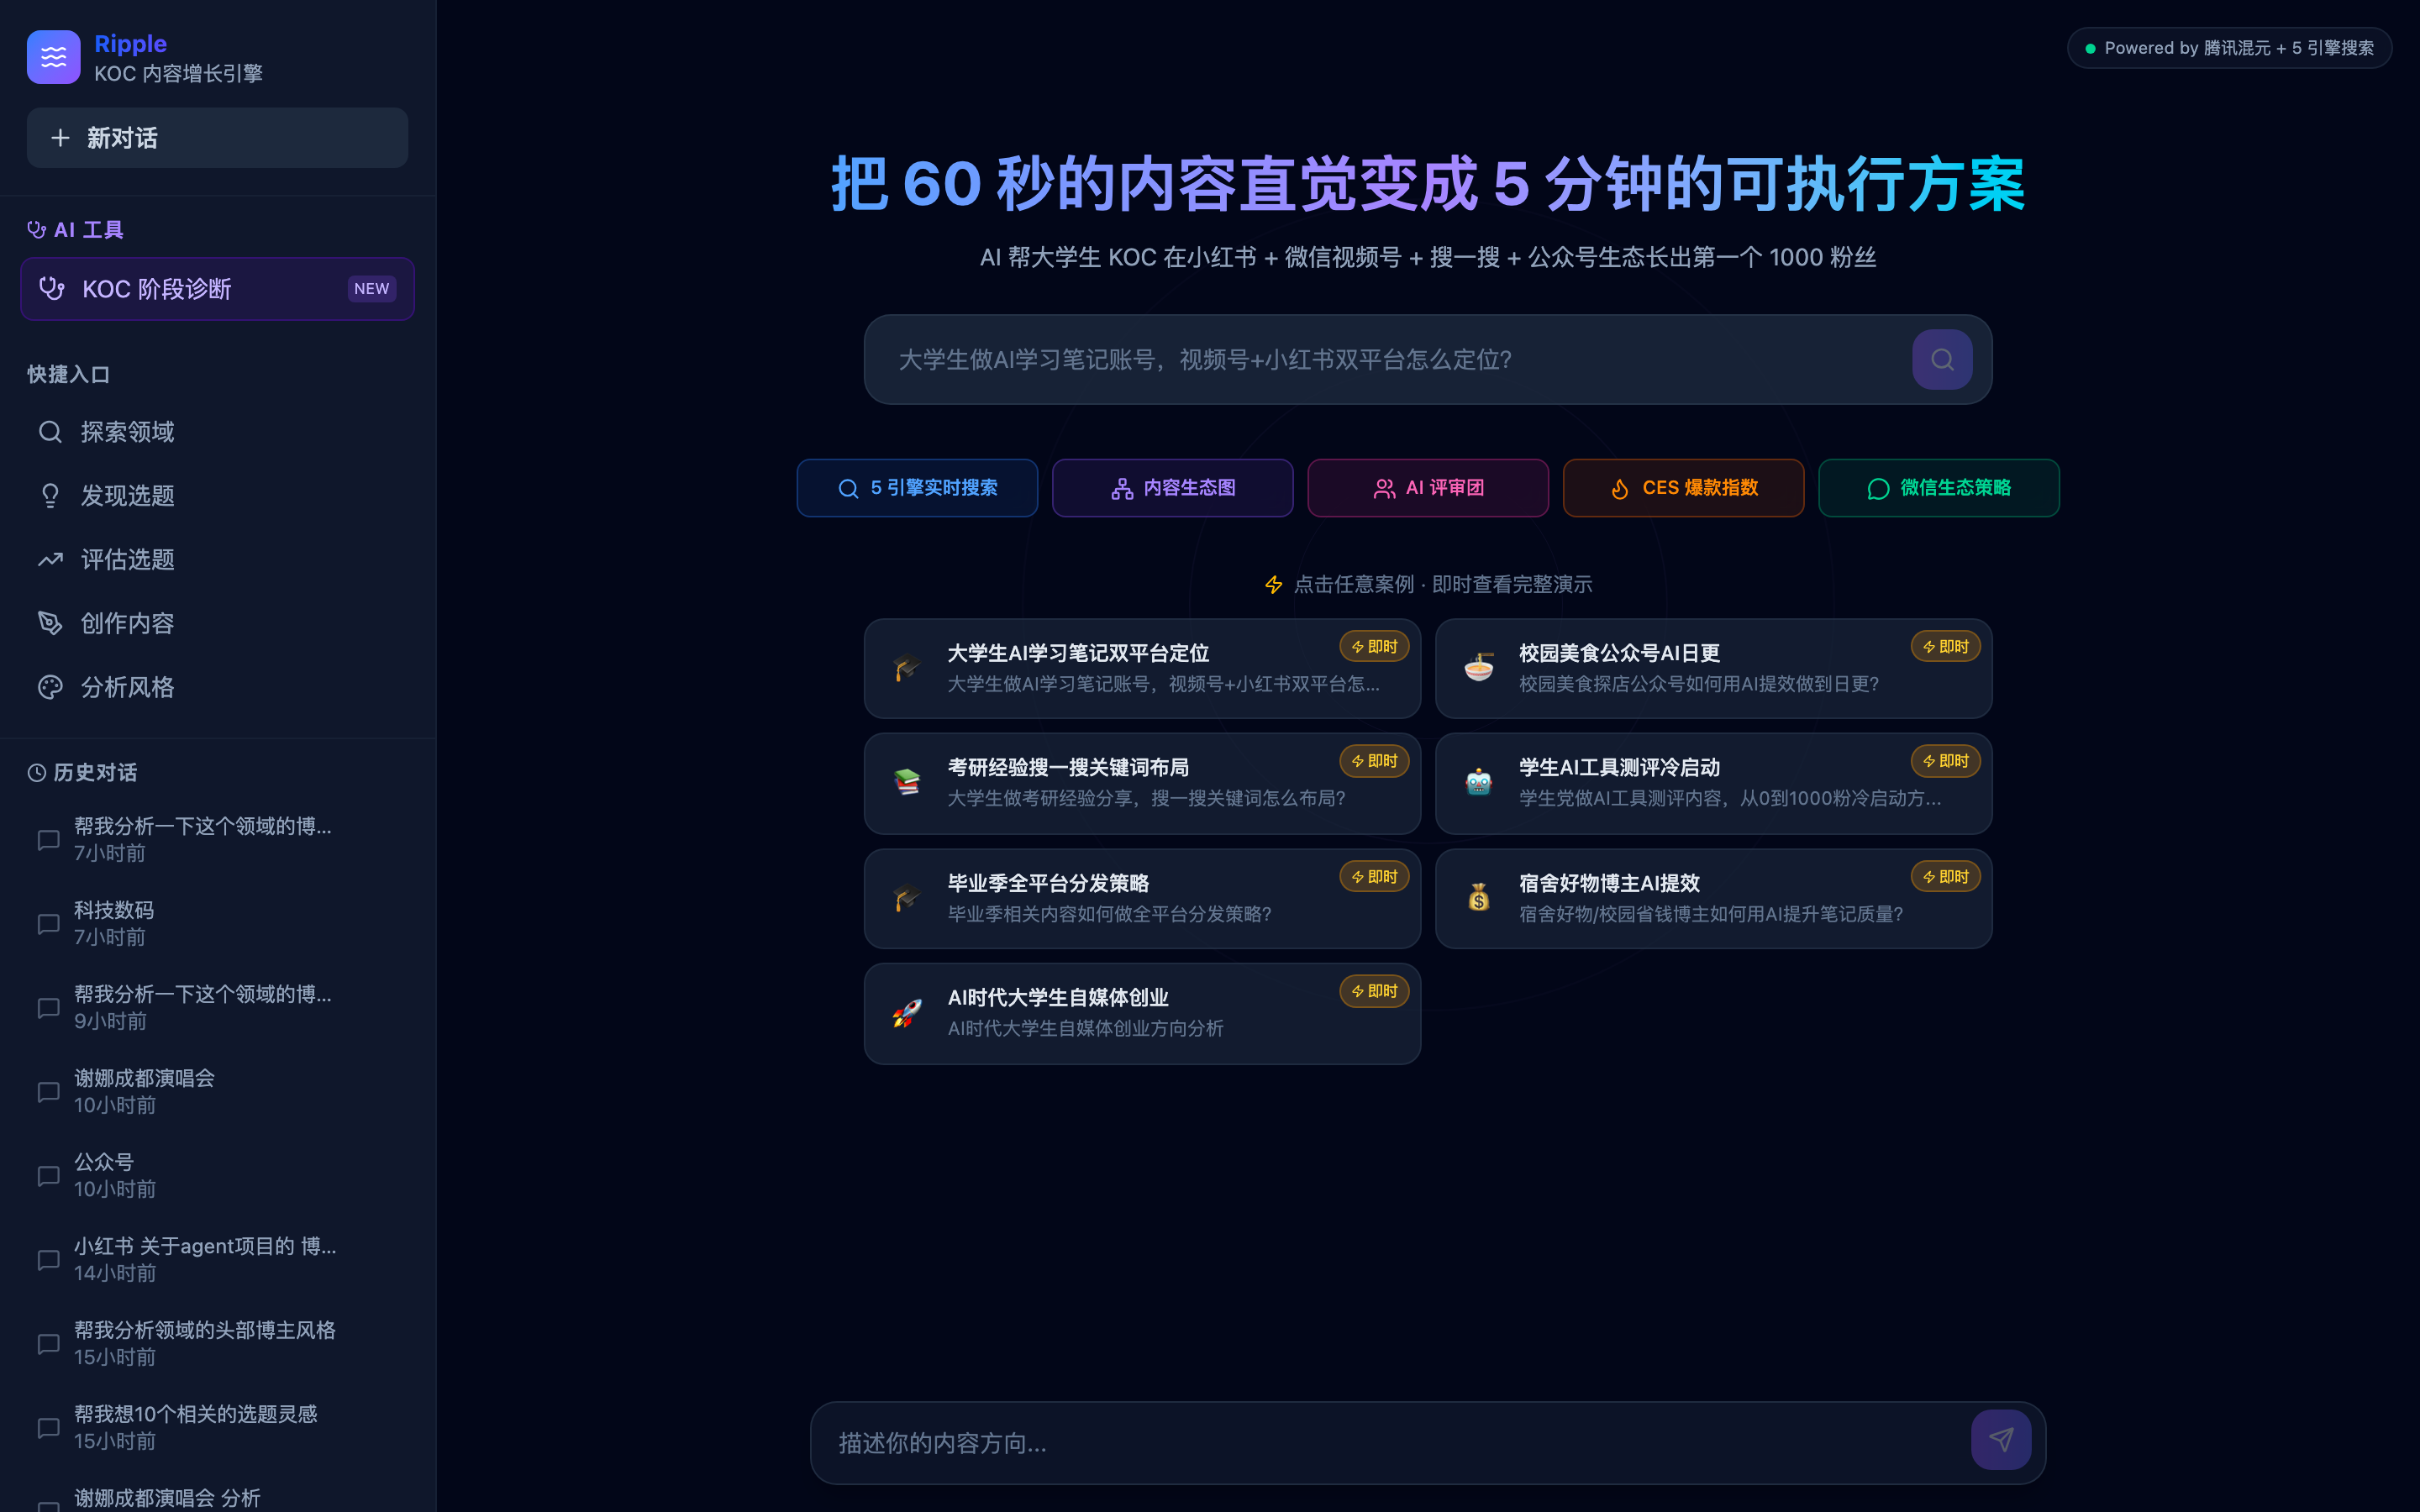
\includegraphics[width=14cm,keepaspectratio]{screenshots/hero.png}
\end{center}

\subsection{零学习成本交互设计}

Ripple 的交互设计原则是``不需要教程''——每个功能入口都有自解释的标签和示例：

\begin{itemize}
  \item 输入框有 Placeholder：``尝试：大学生 AI 学习笔记 · 校园美食探店 · 考研经验...''
  \item Demo 卡片直接展示话题、赛道和卖点，一目了然
  \item SSE 流式输出让用户能实时看到 AI 在做什么，消除等待焦虑
  \item 每个分析结果都有明确的``下一步行动''区域
\end{itemize}


\section{核心功能模块用户体验详解}

\subsection{功能一：多源实时搜索}

用户输入话题后，系统立即显示：
\begin{itemize}
  \item ``正在搜索 5 个来源...''进度提示
  \item 搜索完成后显示来源统计：``已从 MiniMax、Google、Tavily 等获取 18 条相关内容''
  \item 每条引用内容均带来源链接，用户可追溯原文
\end{itemize}

交互细节：引用以``Source 卡片''形式嵌入在流式内容中，而非单独的脚注区，
用户阅读时即可感知信息的真实来源，增强可信度。

\subsection{功能二：内容生态图谱（图文说明）}

\begin{center}
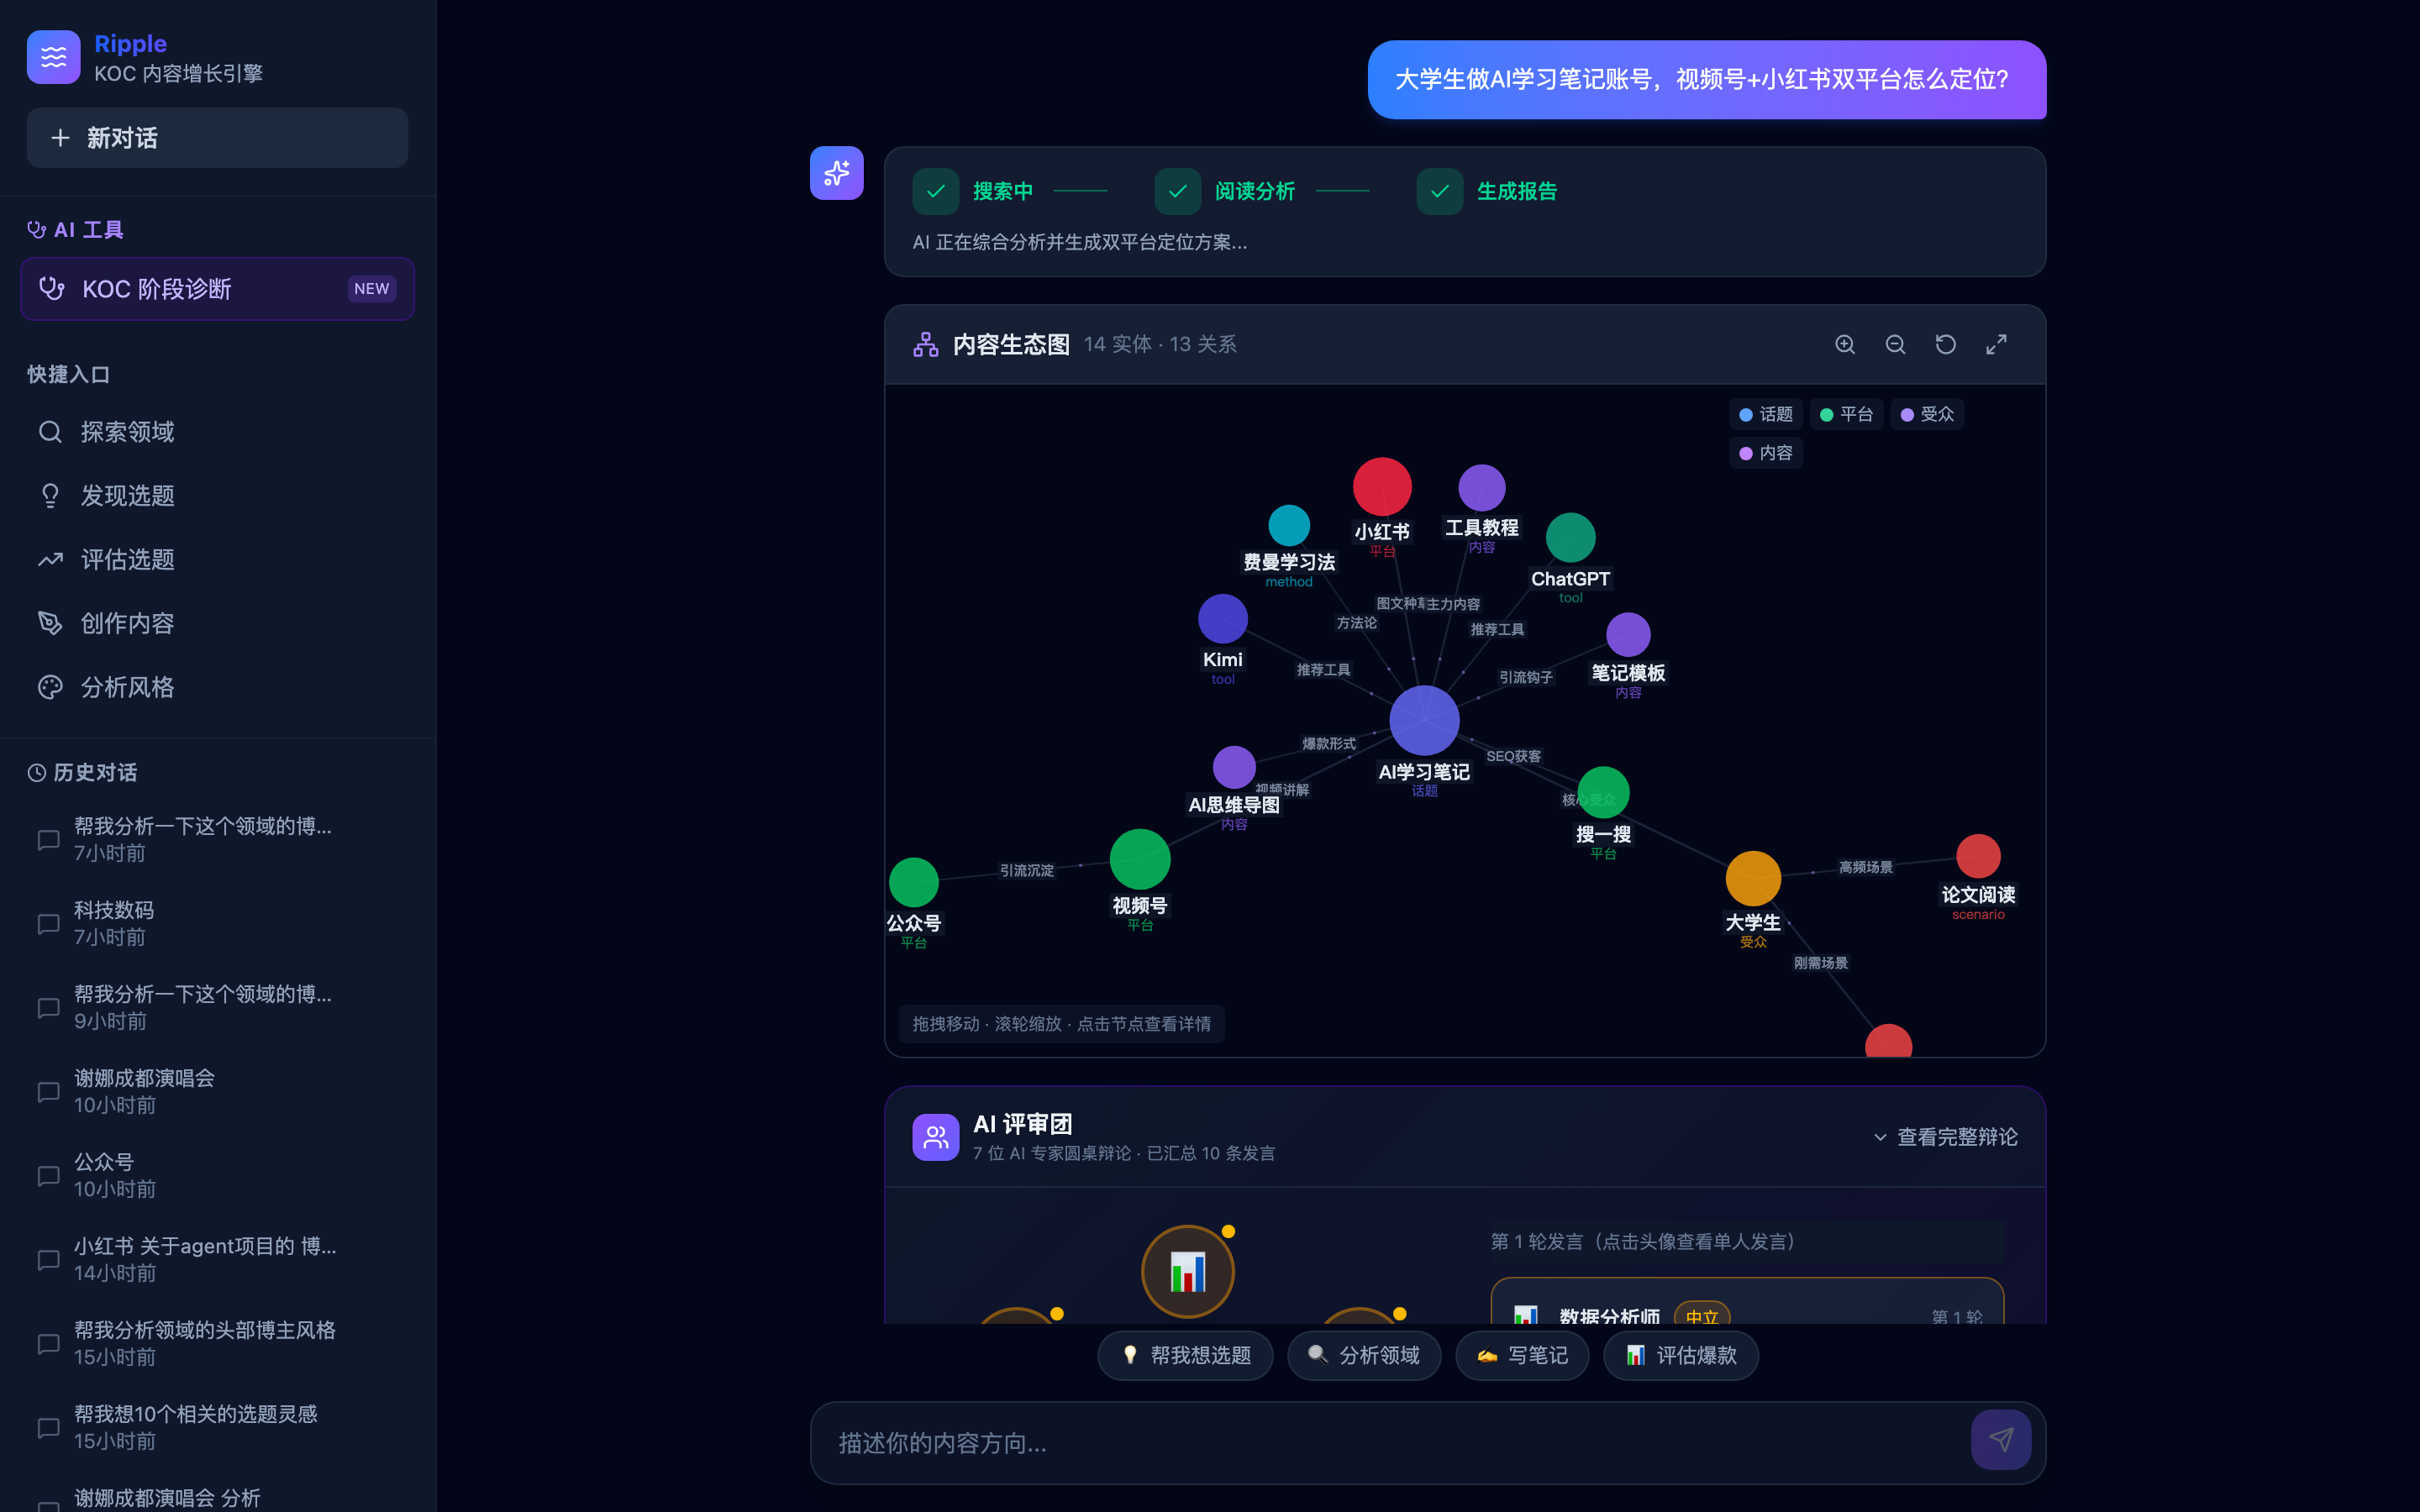
\includegraphics[width=14cm,keepaspectratio]{screenshots/content_eco.png}
\end{center}

\textbf{用户操作路径：}
\begin{enumerate}
  \item 输入话题（如``大学生 AI 工具测评''），等待 8-12 秒
  \item 图谱自动渲染：60 个节点，按类型用 14 种颜色区分
  \item 点击任意节点查看详情面板（实体描述 + 重要度分 + 相关建议）
  \item 悬停显示该节点的所有关联关系
  \item 工具栏可一键缩放全局 / 重置布局 / 展开子图
\end{enumerate}

\textbf{设计亮点：}
不同节点类型用颜色直觉区分（黄色=话题、绿色=平台、紫色=人物），
用户无需看图例就能快速理解图谱结构。

\subsection{功能三：AI 专家圆桌（图文说明）}

\begin{center}
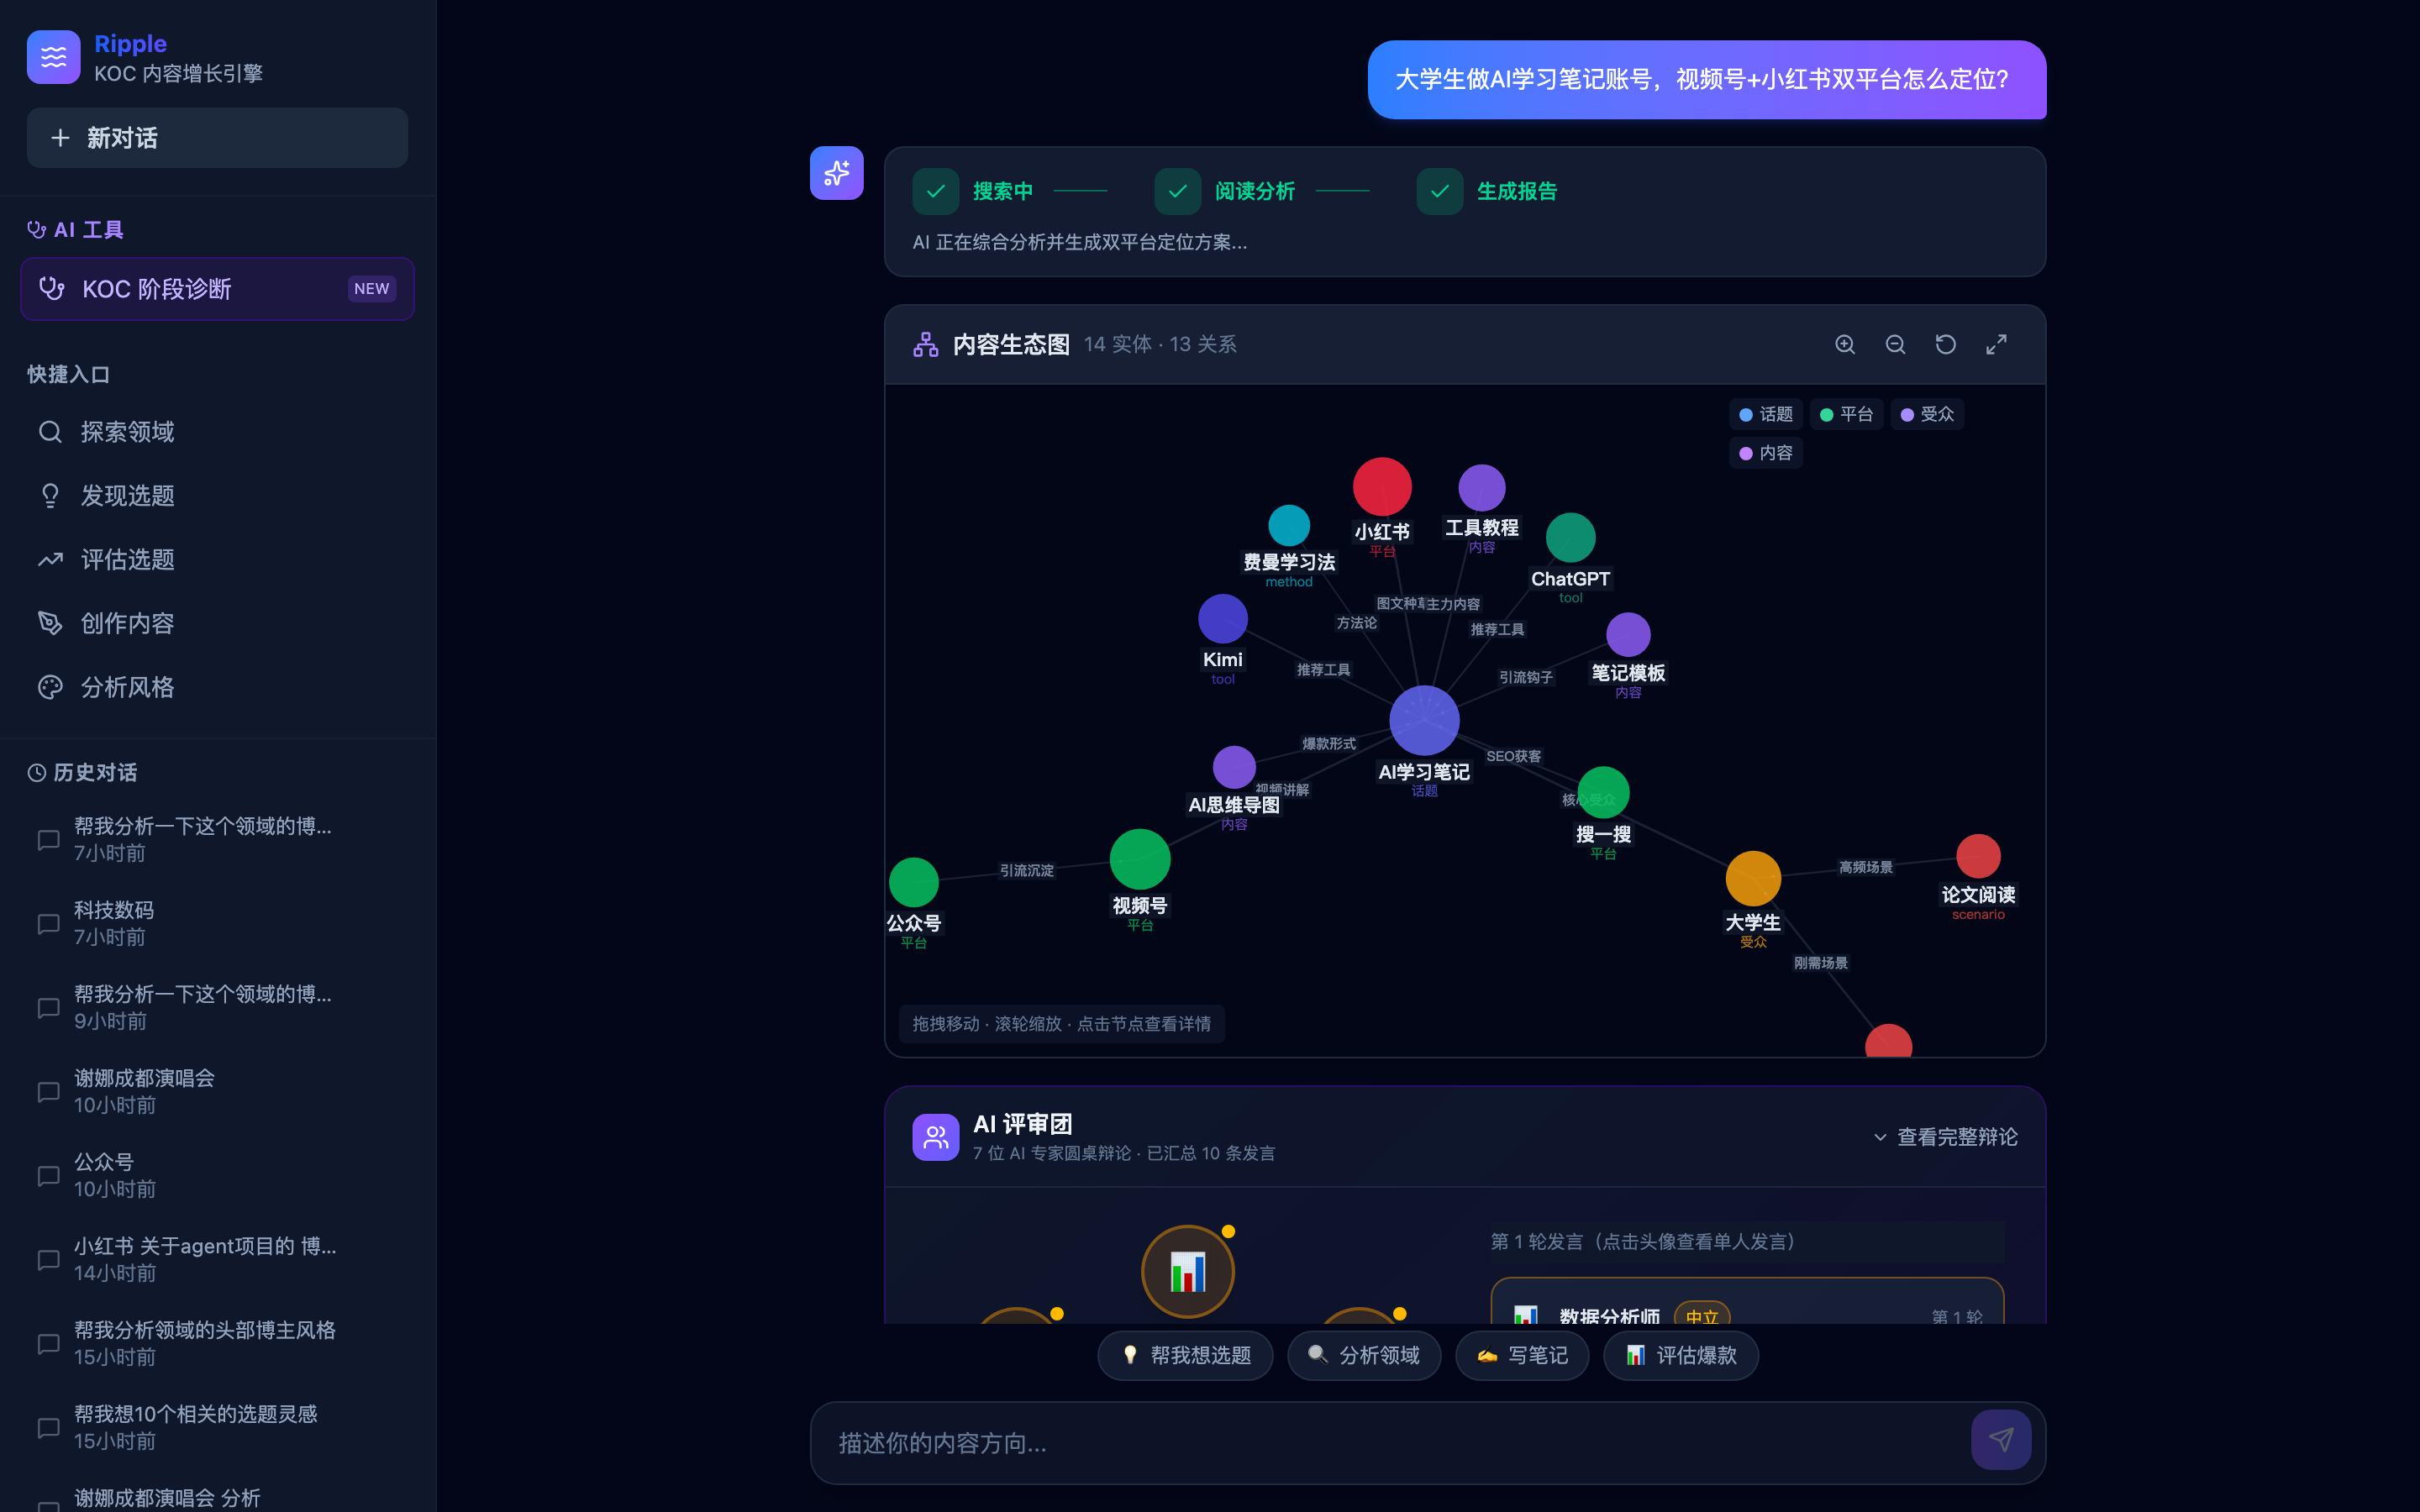
\includegraphics[width=14cm,keepaspectratio]{screenshots/roundtable.png}
\end{center}

\textbf{体验亮点：}
\begin{itemize}
  \item 7 个专家头像以环形排列，有发言的头像会有动态光圈
  \item 点击任一头像展开完整发言（200-300 字精练观点）
  \item 态度标签（[看好] / [中立] / [谨慎]）一目了然地显示在头像下方
  \item 共识度进度条（0-100\%）随讨论进行实时更新
  \item 仲裁者卡片用金色边框突出显示，最终建议包含：评分 + 核心风险 + 机会 + 立即行动
\end{itemize}

\subsection{功能四：CES 爆款指数仪表盘（图文说明）}

\begin{figure}[htbp]
\centering
\begin{subfigure}[b]{0.48\textwidth}
  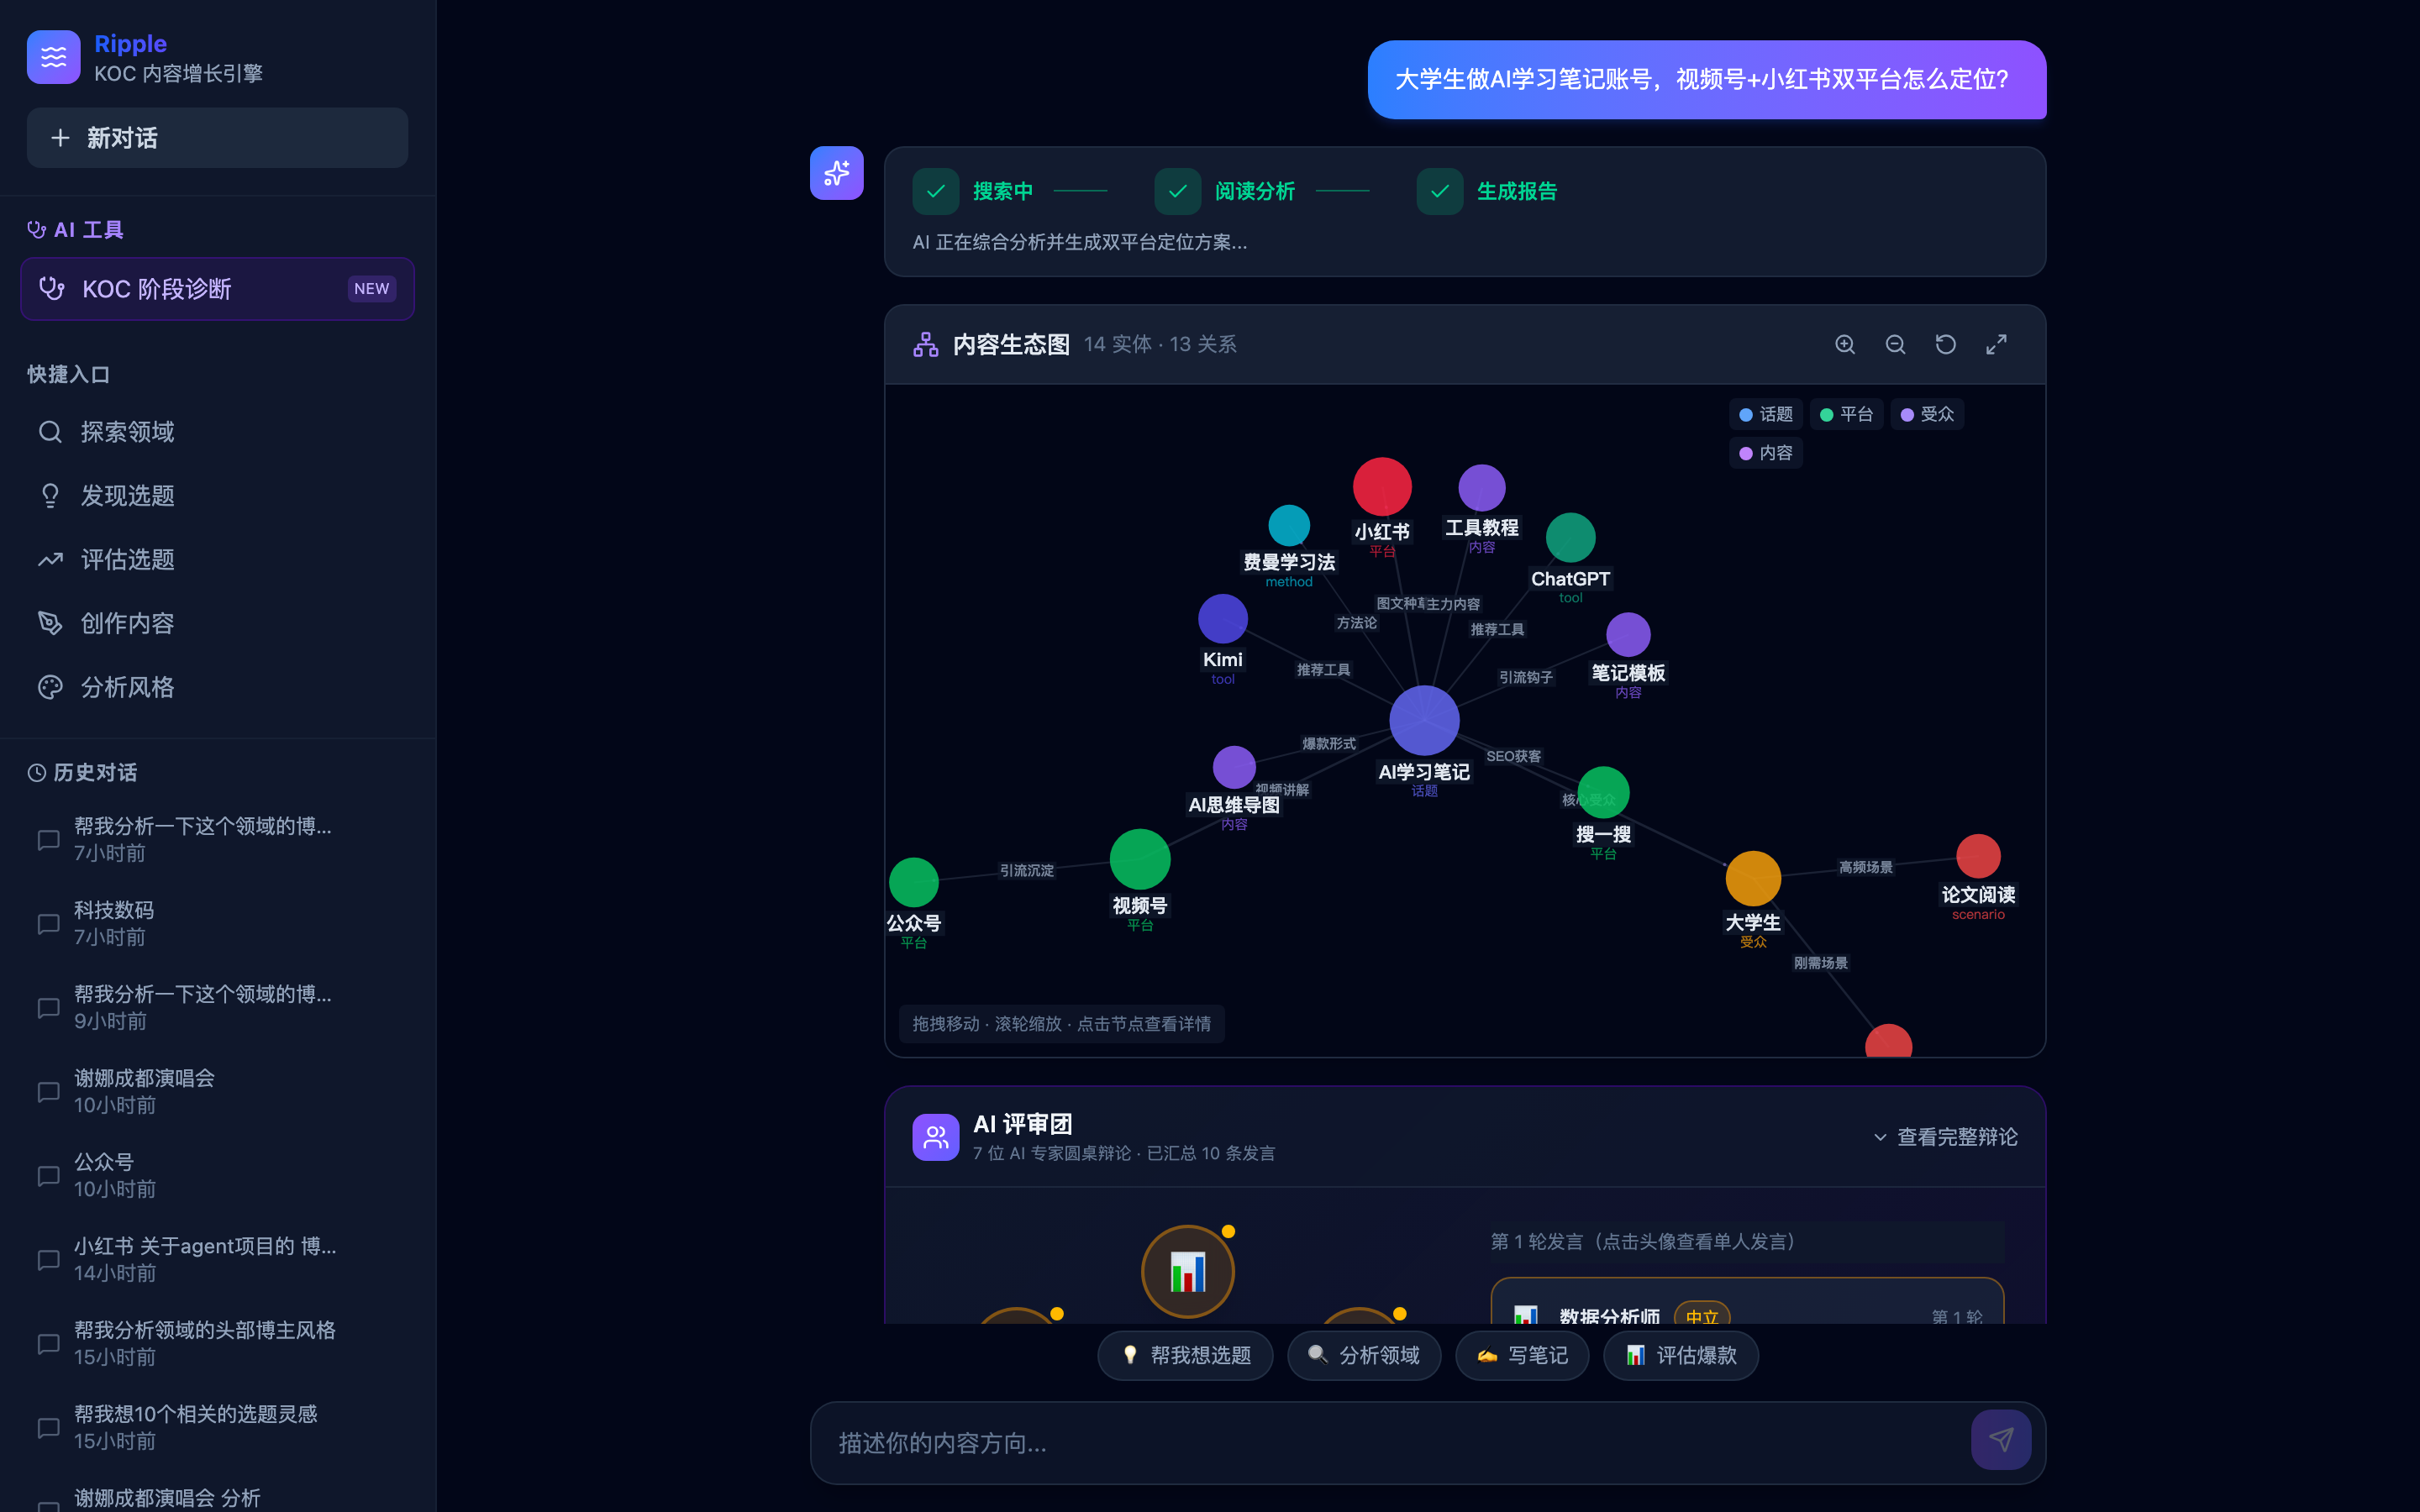
\includegraphics[width=6.5cm,keepaspectratio]{screenshots/ces_dash.png}
\end{subfigure}
\hfill
\begin{subfigure}[b]{0.48\textwidth}
  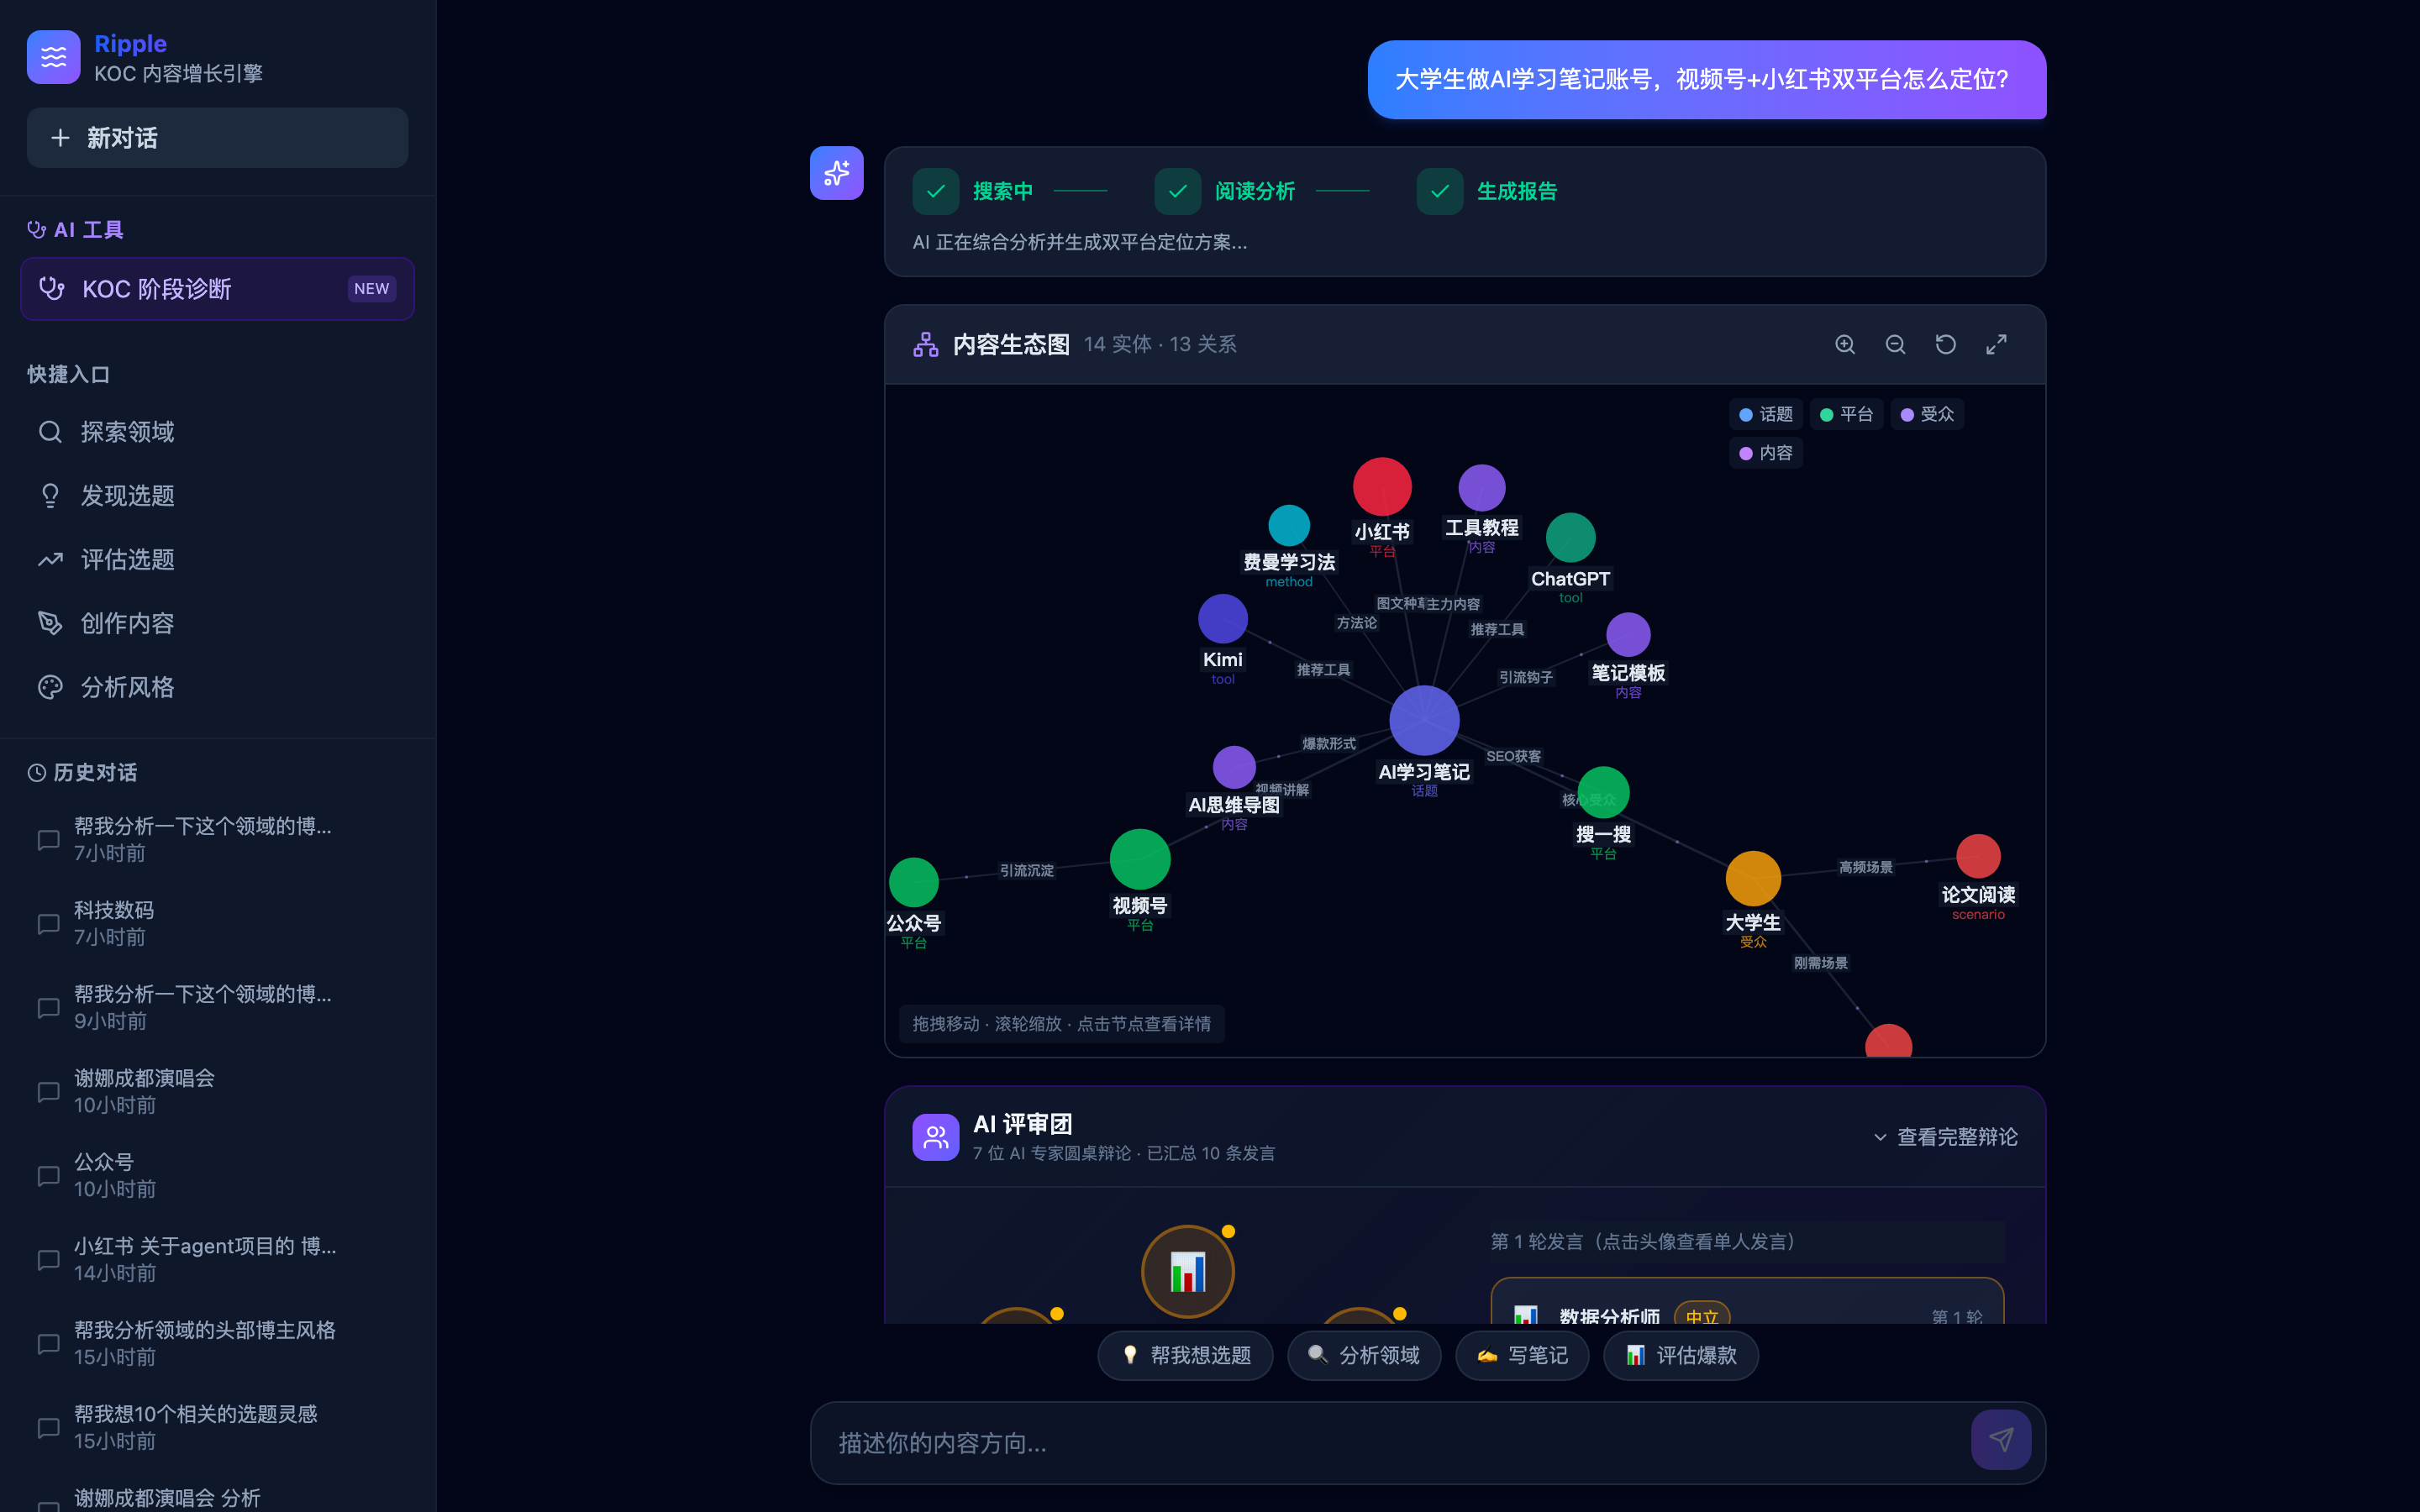
\includegraphics[width=6.5cm,keepaspectratio]{screenshots/ces_slider.png}
\end{subfigure}
\caption{CES 爆款指数模拟器}
\end{figure}

\textbf{交互体验设计：}
\begin{itemize}
  \item 19 维雷达图直观展示各维度得分（哪个维度弱一眼可见）
  \item 综合分数大字显示（如 72/100），配合``进入初级流量池''的文字判断
  \item 5 个滑块代表 5 种互动行为，拖动后雷达图和分数实时更新（无需重新提交）
  \item 30 天增长曲线用面积图展示，并标注各阶段转折点
  \item 改进建议针对最低分维度给出具体可执行的优化方向
\end{itemize}

\subsection{功能五：微信生态四面板（图文说明）}

\begin{figure}[htbp]
\centering
\begin{subfigure}[b]{0.48\textwidth}
  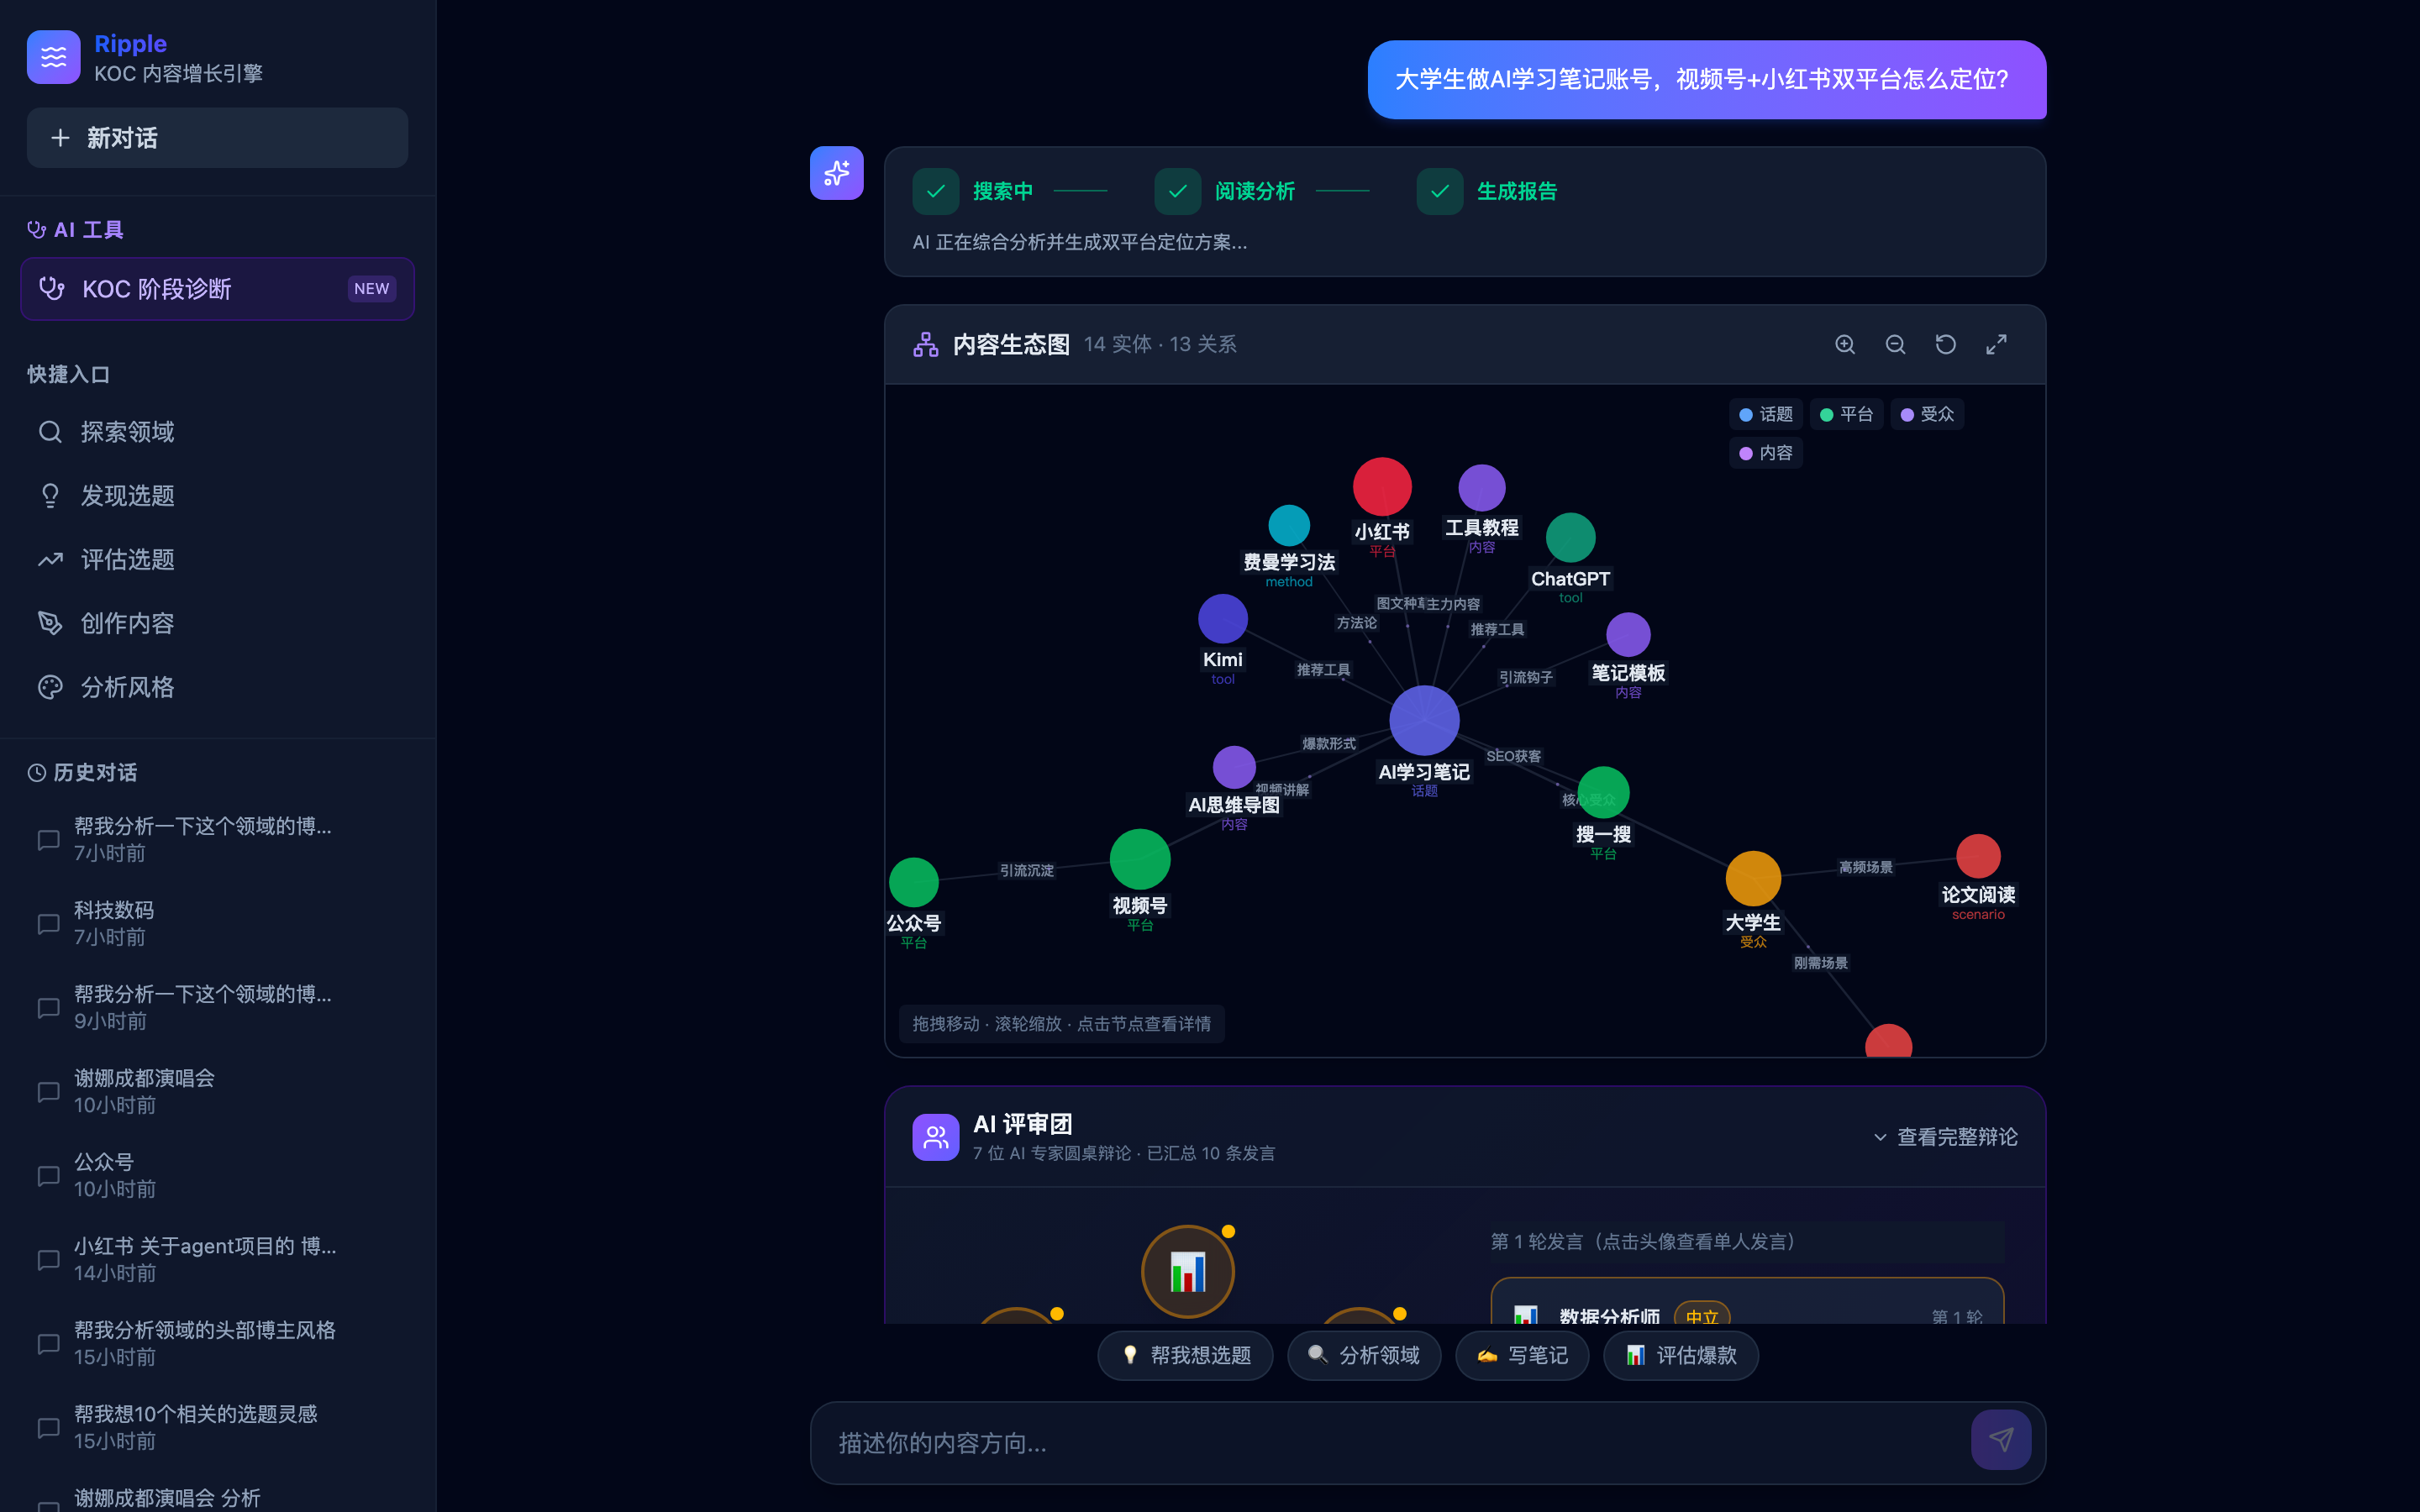
\includegraphics[width=6.5cm,keepaspectratio]{screenshots/wechat_search.png}
\end{subfigure}
\hfill
\begin{subfigure}[b]{0.48\textwidth}
  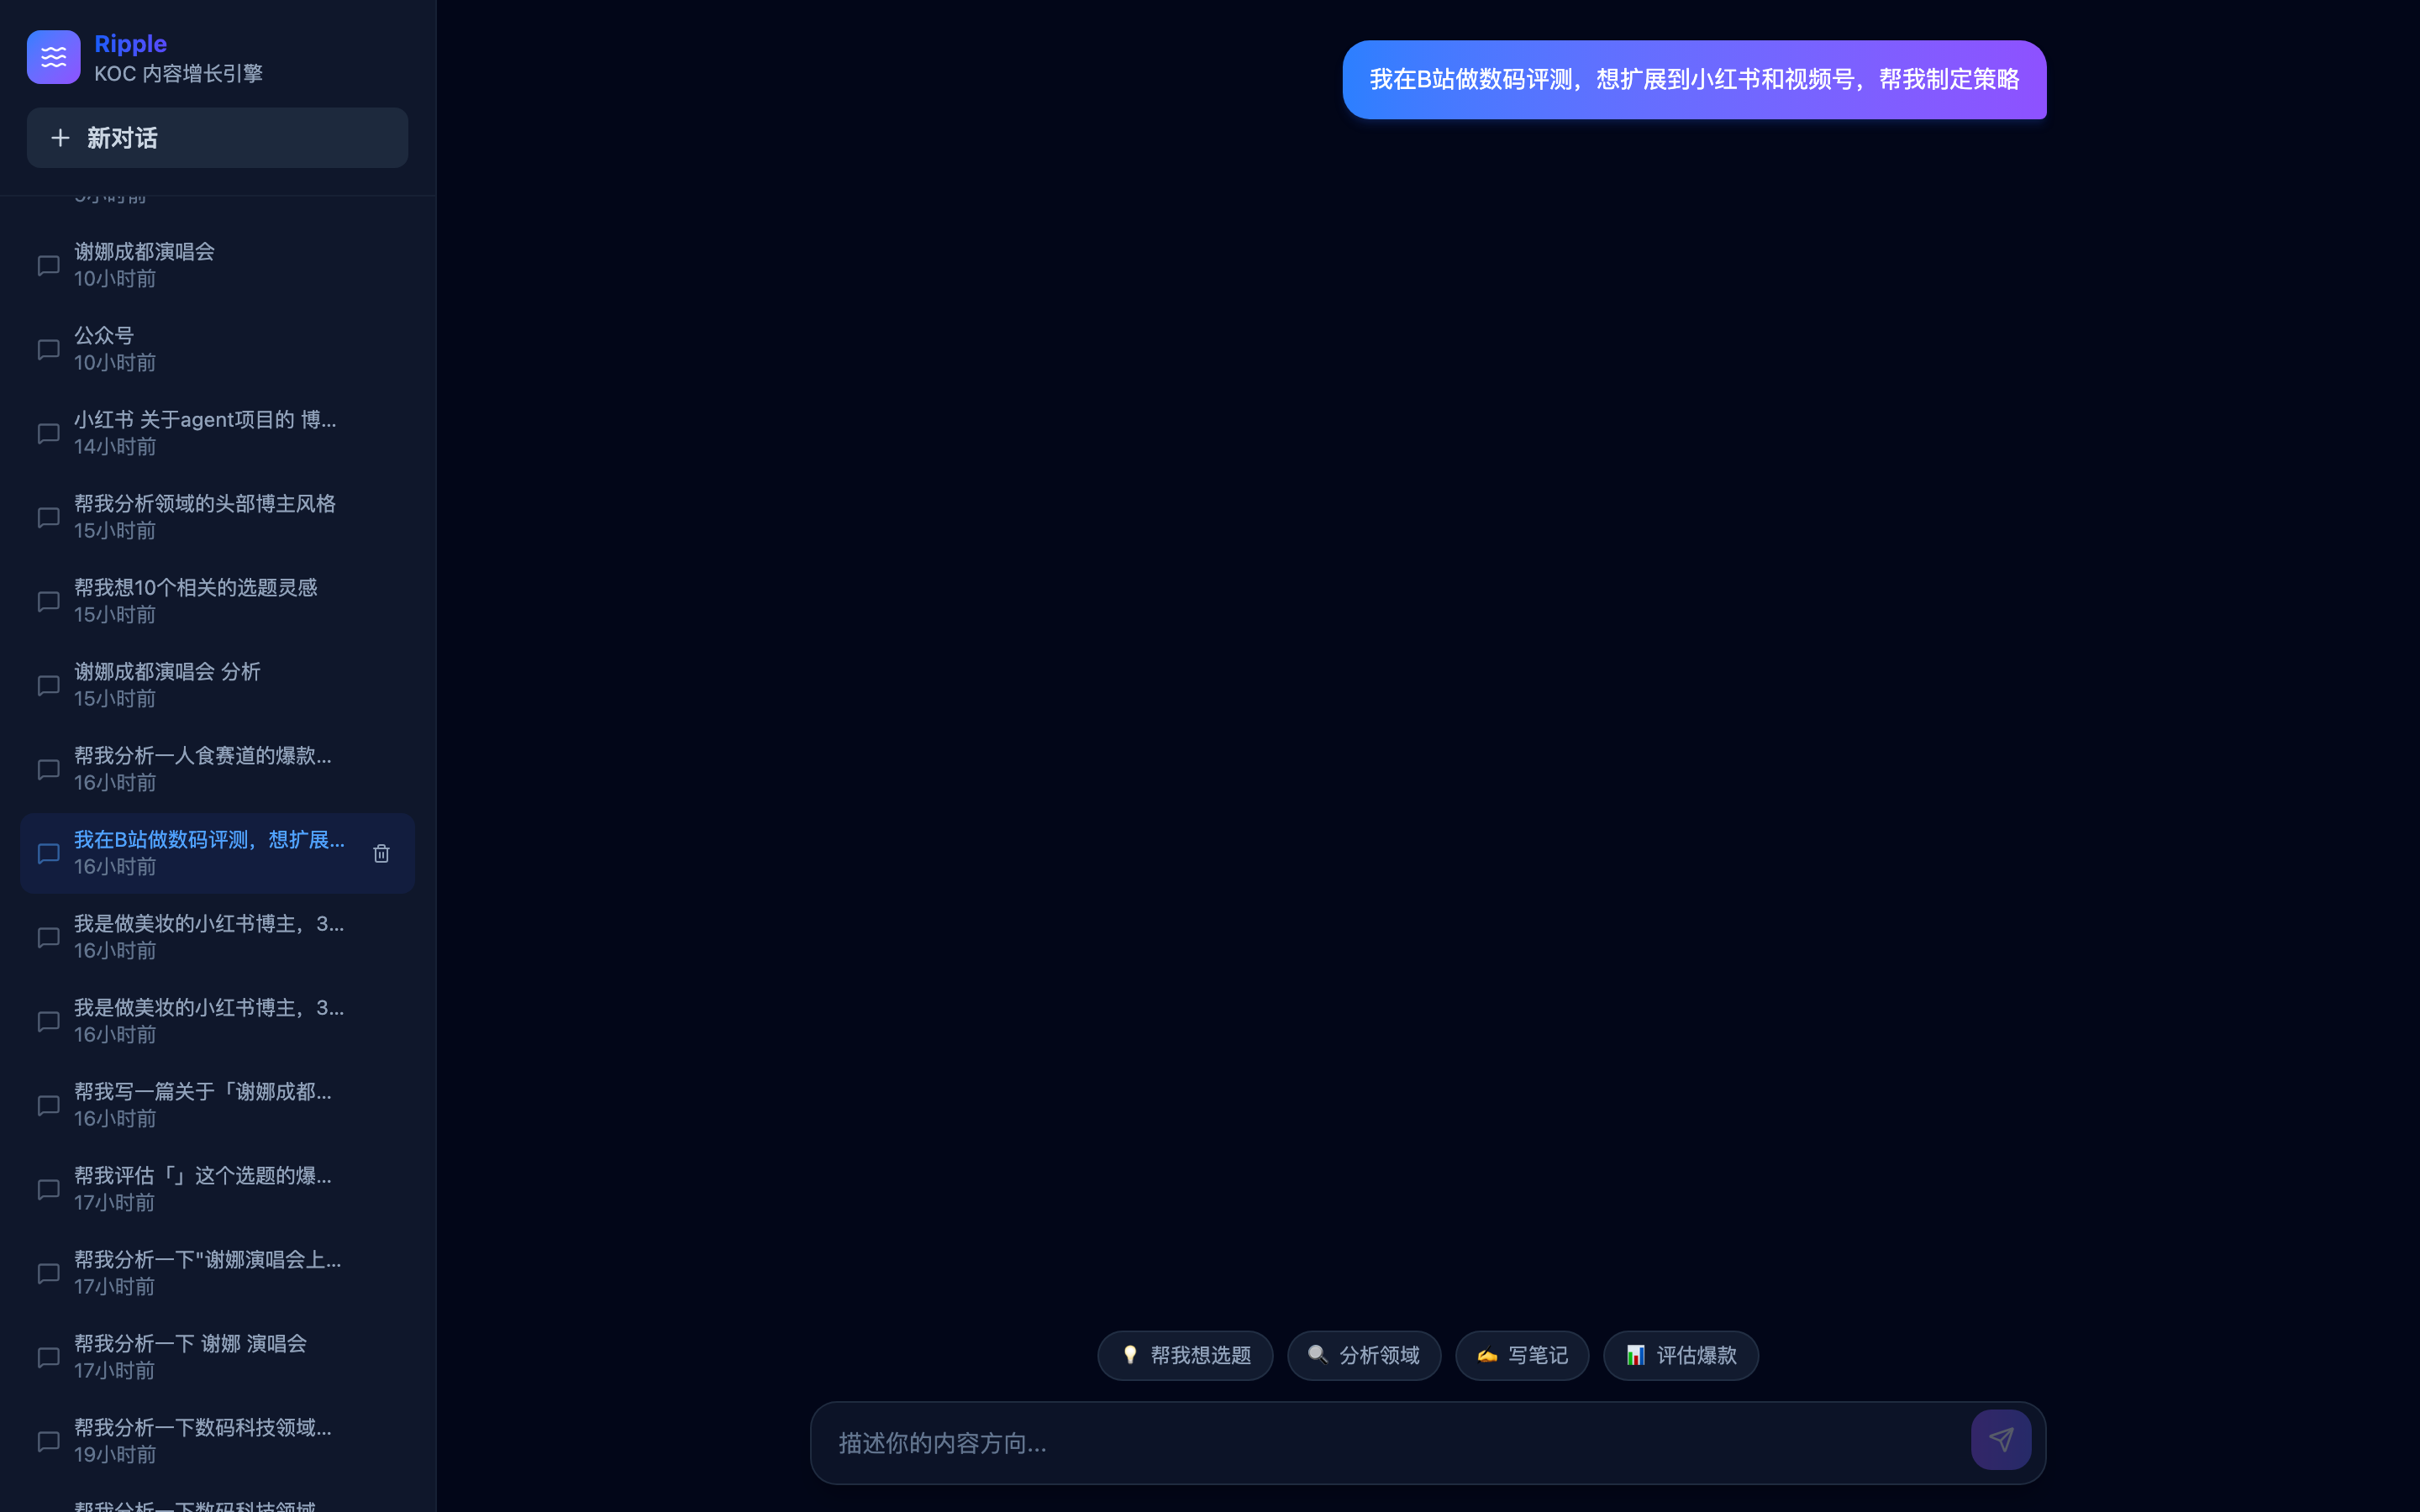
\includegraphics[width=6.5cm,keepaspectratio]{screenshots/wechat_video.png}
\end{subfigure}
\caption{微信生态分析面板}
\end{figure}

四个子面板按 Tab 切换，每个面板都有独立的交互逻辑：
\begin{itemize}
  \item \textbf{搜一搜}：输入关键词，柱状图对比 5 个相关词的搜索量和竞争度
  \item \textbf{视频号}：选择社交圈层规模，社交链路图展示内容扩散路径
  \item \textbf{公众号}：关键词热图，颜色深浅代表标题不同位置的权重
  \item \textbf{私域}：KOC 金字塔，拖动滑块模拟不同阶段的用户层级分布
\end{itemize}

\subsection{功能六：KOC 阶段诊断（图文说明）}

\begin{center}
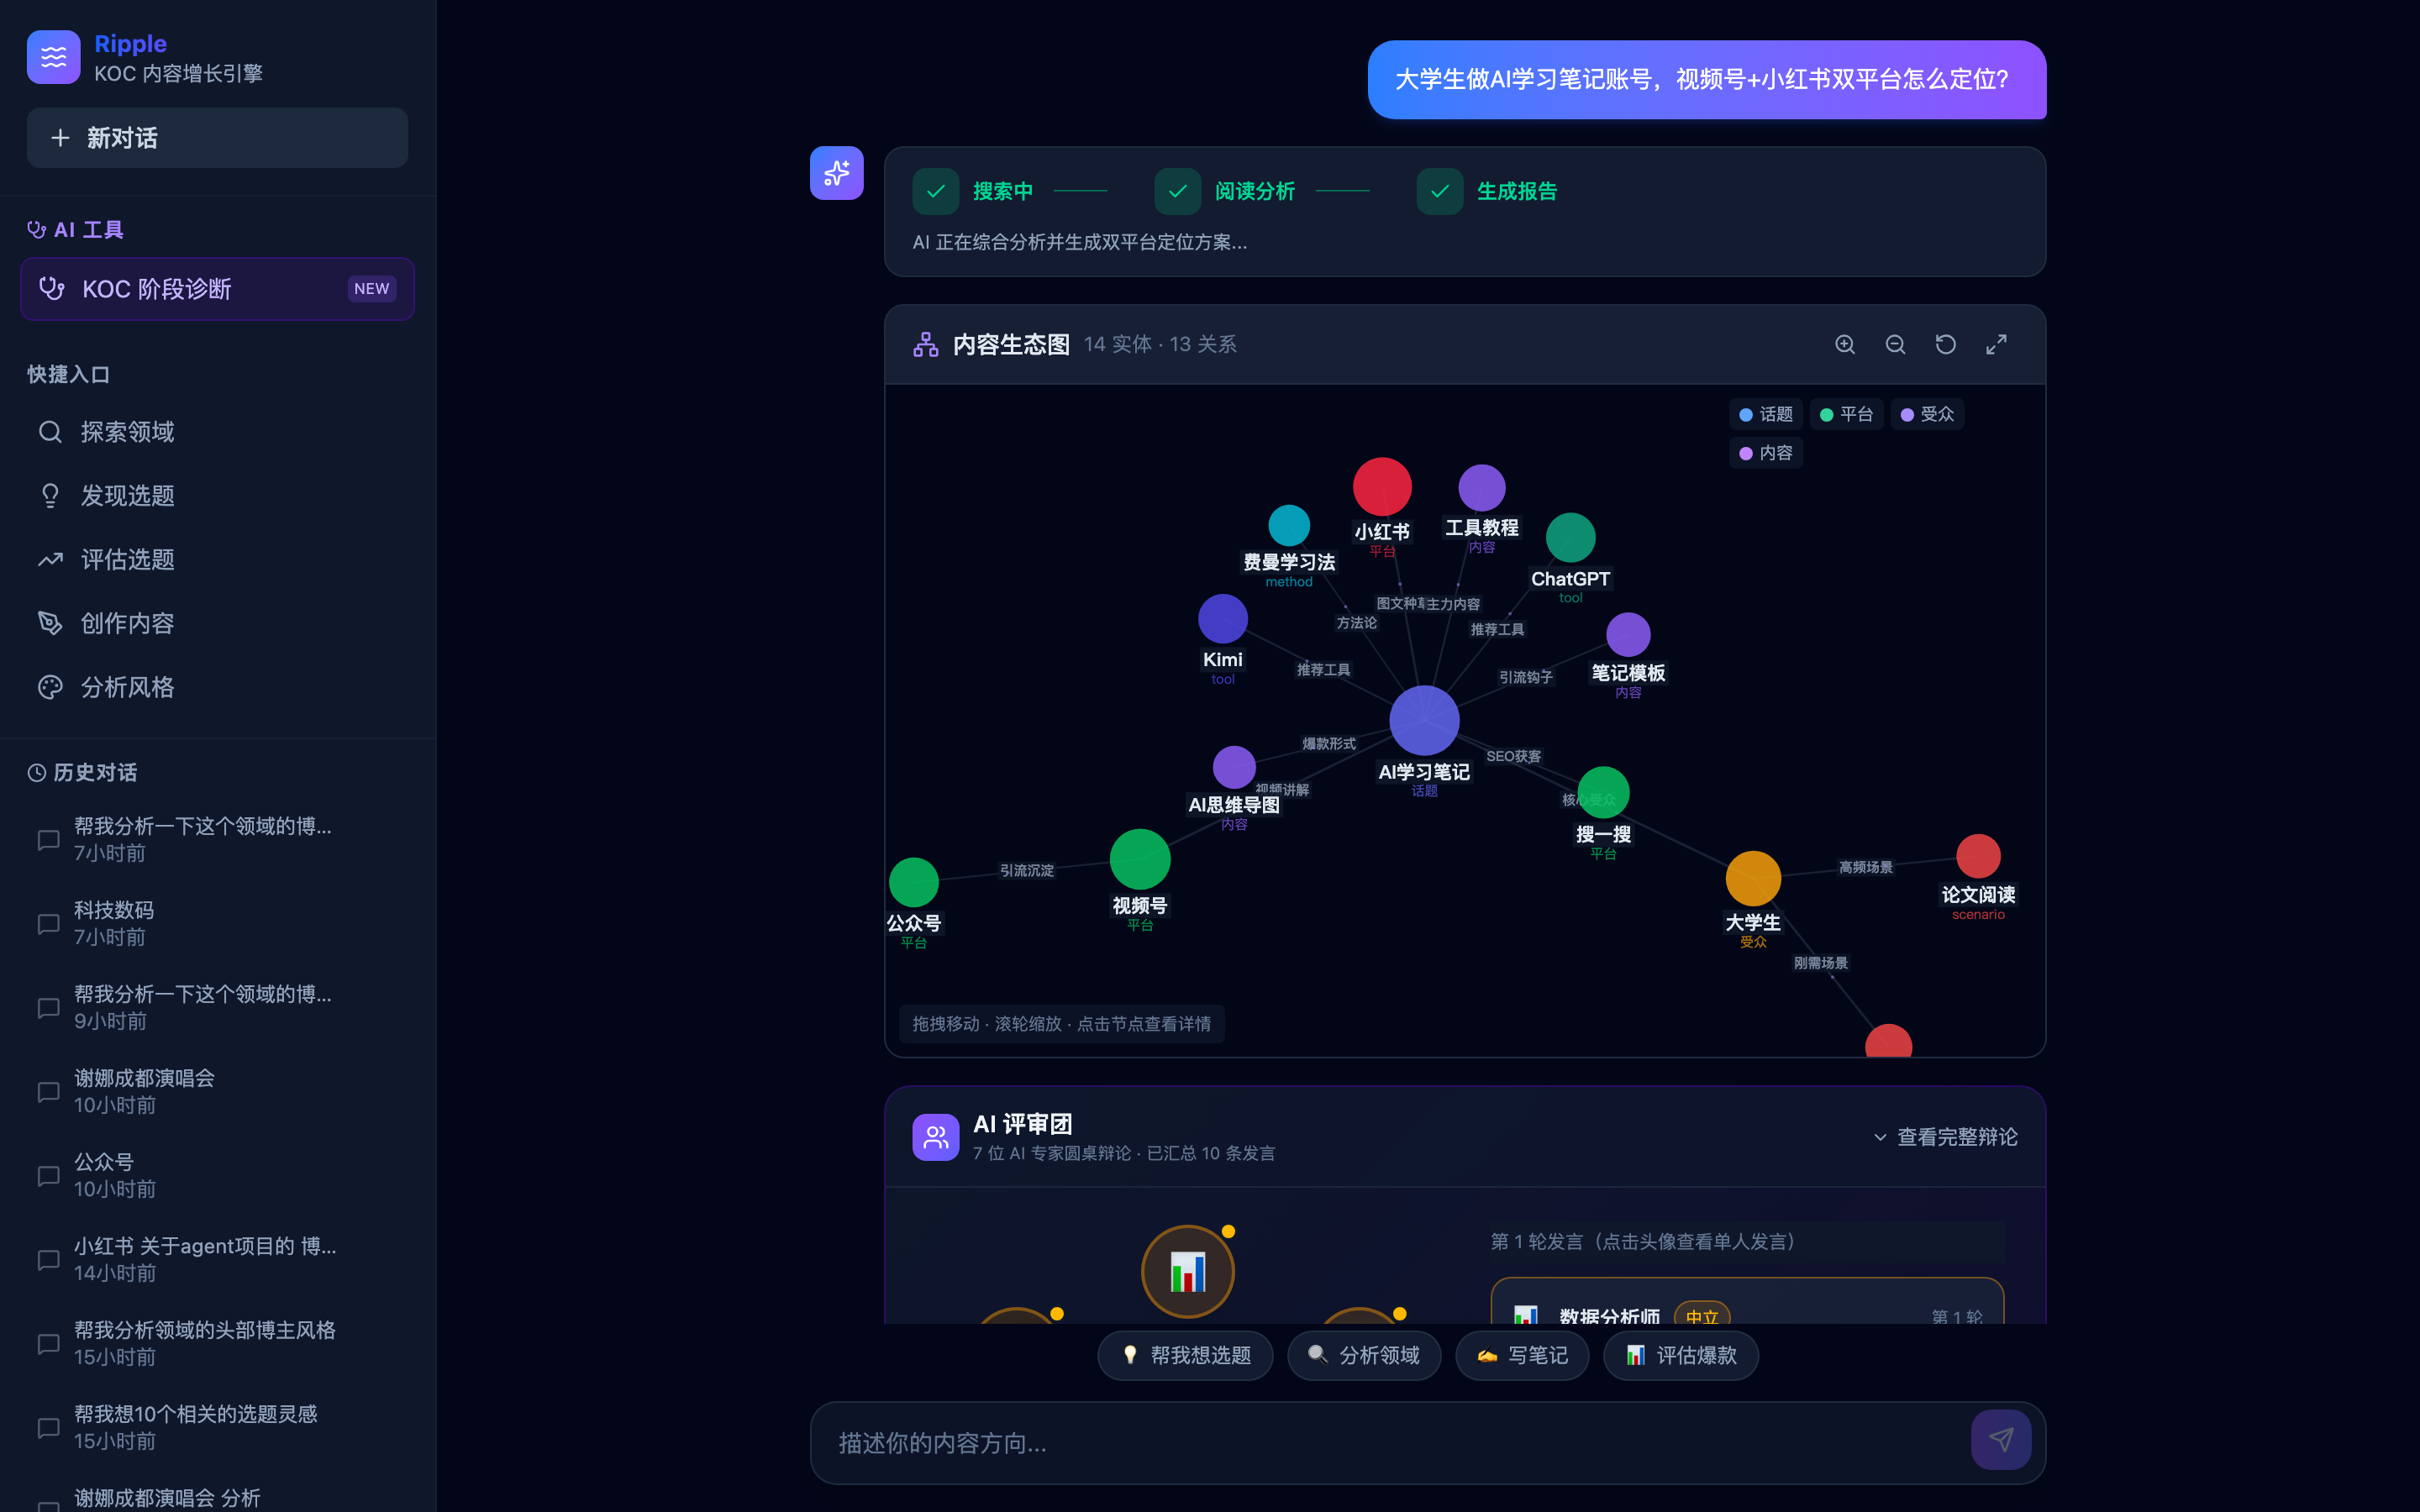
\includegraphics[width=14cm,keepaspectratio]{screenshots/koc_diagnose.png}
\end{center}

\textbf{用户操作路径：}
\begin{enumerate}
  \item 输入：粉丝数量、平均点赞、近 30 天发布数量、主要平台
  \item Ripple 自动判断：``你处于\textbf{成长期（100-1000 粉）}''
  \item 展示健康度四维评分：互动率 65分 / 更新频率 70分 / 内容垂直度 80分 / 涨粉速度 55分
  \item 突破三步法：``1. 固定每周三和周六发布，建立用户预期...''
\end{enumerate}

\subsection{功能七：多平台一键导出}

\begin{figure}[htbp]
\centering
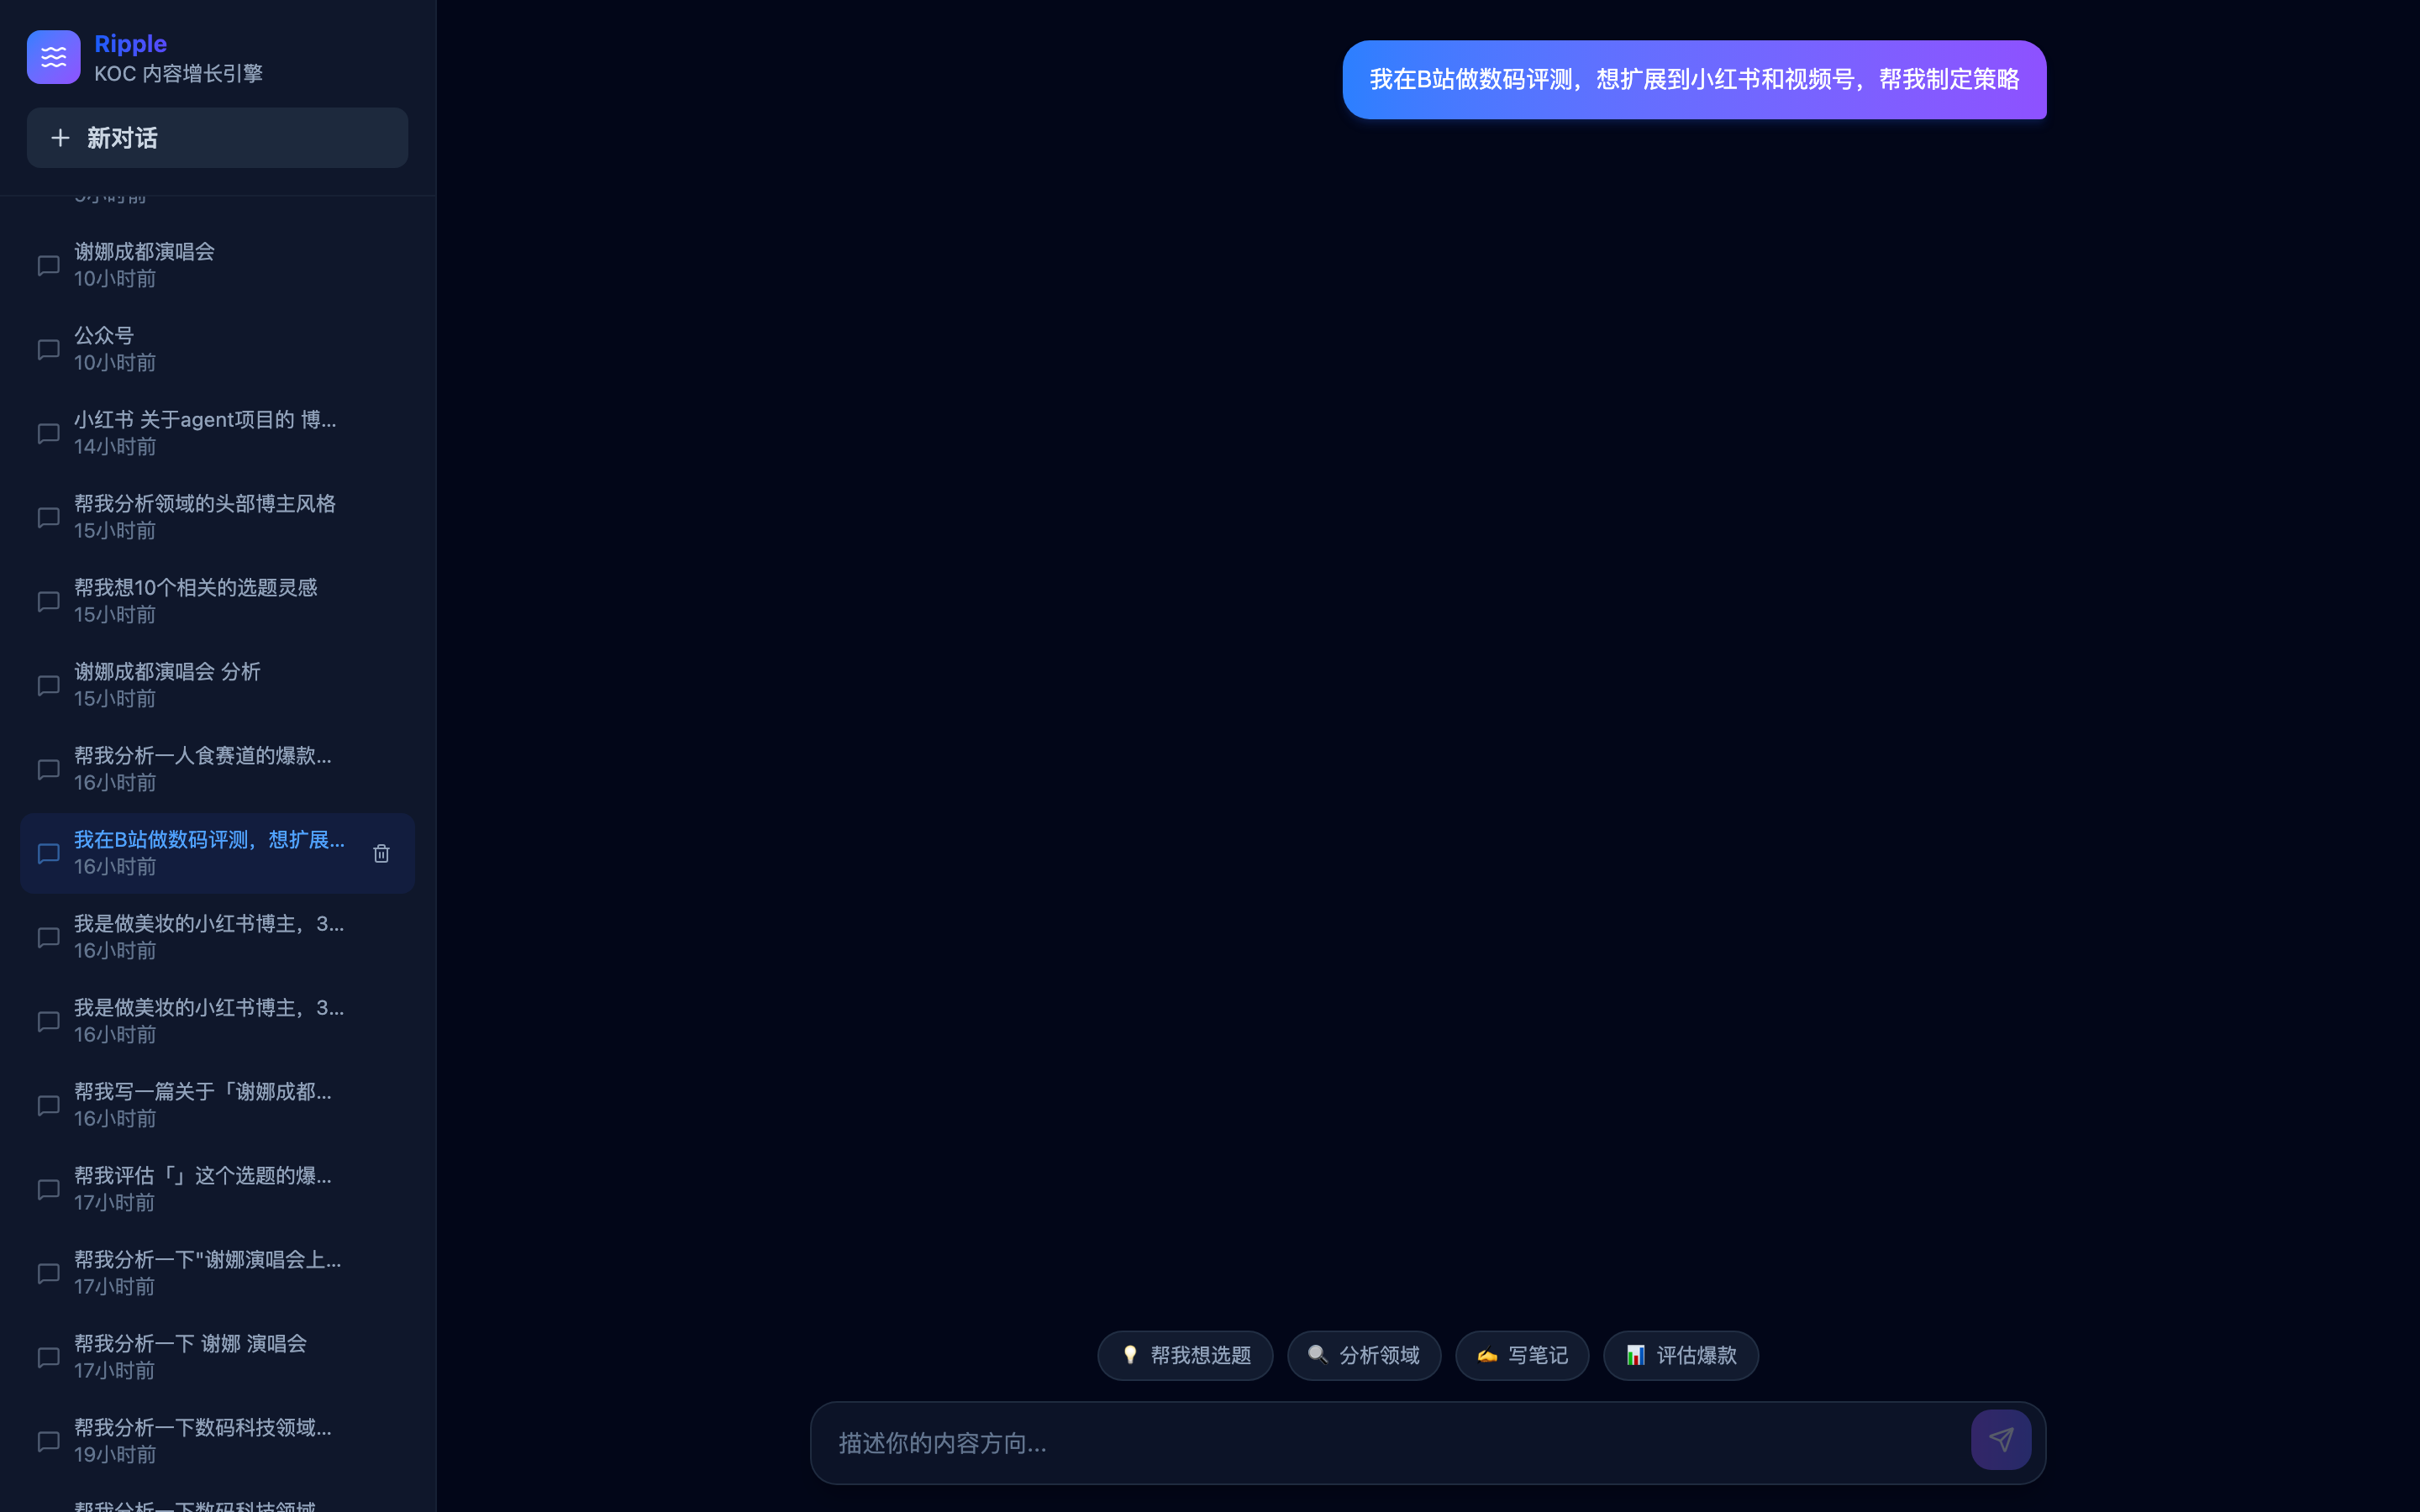
\includegraphics[width=8cm,keepaspectratio]{screenshots/copy_export.png}
\caption{多平台格式一键复制}
\end{figure}

\textbf{四种输出格式：}
\begin{itemize}
  \item \textbf{小红书格式}：emoji 开头 + 分段短句 + \#话题标签 + @提及
  \item \textbf{视频号脚本}：Hook（前 3 秒）+ 主体（内容节奏）+ CTA（引导关注）
  \item \textbf{公众号正文}：标题 H1 + 正文分段 + 小标题 + 关注引导语
  \item \textbf{原文 Markdown}：完整分析报告，适合存档或二次编辑
\end{itemize}

每种格式一个按钮，点击即复制到剪贴板，配合提示动画``已复制！''。


\section{Demo 案例详细介绍}

Ripple 内置 6 个针对大学生 KOC 场景的完整 Demo，每个 Demo 预载了全套 Mock 数据，
点击后 $<$1 秒即可看到完整的分析结果（无需等待 AI 生成）。

\subsection{Demo 1：大学生 AI 学习笔记双平台定位}

\textbf{赛道：}教育 \quad \textbf{目标平台：}小红书 + 公众号

\textbf{核心卖点：}双平台差异化内容策略——同一话题在小红书用视觉化笔记吸引新用户，
在公众号用深度文章建立专业形象。适合技术型学生 KOC 的``两条腿走路''策略。

\textbf{展示内容：}
\begin{itemize}
  \item 内容生态图：AI 学习、工具测评、笔记分享、教育类 KOC 的关系图谱
  \item CES 评分：标题``大学生 1 个月用 AI 提效 300\% 的完整方法''评分 85 分
  \item 圆桌讨论：数据分析师强烈看好（AI 工具赛道红利期），风险评估师提示内容同质化风险
  \item 微信策略：搜一搜关键词``AI 学习方法''月搜索量 23 万，竞争度中等，建议布局
\end{itemize}

\subsection{Demo 2：校园美食探店日更}

\textbf{赛道：}本地生活 \quad \textbf{目标平台：}小红书 + 视频号

\textbf{核心卖点：}AI 驱动的全链路效率提升——从选店（用 AI 查评价）到拍摄（AI 提示构图）
到发布（AI 生成文案），日更不再累人。

\textbf{特色展示：}
\begin{itemize}
  \item 本地 SEO 策略：搜索词``XX 大学周边 + 探店''的精准覆盖路径
  \item 视频号社交链路：校园内熟人关系链对本地内容的天然放大效应
  \item KOC 诊断：处于``成长期''，建议固定同一时间段发布建立本地用户习惯
\end{itemize}

\subsection{Demo 3：考研经验关键词布局}

\textbf{赛道：}教育 \quad \textbf{目标平台：}搜一搜 + 小红书

\textbf{核心卖点：}搜一搜三级关键词体系——核心词``考研经验''$\rightarrow$
二级词``25 考研数学 / 英语''$\rightarrow$三级词``零基础考研 / 院校选择''，
精确布局高搜索量低竞争词。

\subsection{Demo 4：学生 AI 工具测评冷启动}

\textbf{赛道：}AI \quad \textbf{目标平台：}小红书

\textbf{核心卖点：}0 $\rightarrow$ 1000 粉冷启动方法论。
针对 AI 工具测评这一新兴赛道，Ripple 分析了最佳起步路径：
先发``横向测评对比''类内容快速建立专业形象，再深耕单一工具的深度使用攻略。

\subsection{Demo 5：毕业季全平台分发}

\textbf{赛道：}情感 \quad \textbf{目标平台：}视频号 + 公众号 + 小红书

\textbf{核心卖点：}毕业季天然高传播势能 + 视频号社交链路放大效应。
毕业相关内容在熟人关系链中自然流传，视频号算法中``社交关系链权重 60\%''使此类内容获得超预期传播。

\subsection{Demo 6：宿舍好物 AI 提效}

\textbf{赛道：}消费 \quad \textbf{目标平台：}小红书

\textbf{核心卖点：}CPS 商业化路径 + AI 比价效率。
展示了从内容创作到商业变现的完整路径：
好物推荐 $\rightarrow$ 淘宝/京东联盟 CPS $\rightarrow$ 小红书商品卡片，
Ripple 的 CES 模拟器帮助评估哪类好物内容传播潜力最高。


\section{响应式设计与移动端适配}

\subsection{全设备适配策略}

Ripple 采用 Tailwind CSS 的断点系统实现全设备响应式：

\begin{center}
\begin{tabular}{p{2.5cm} p{3cm} p{3cm} p{5cm}}
\toprule
\textbf{设备} & \textbf{屏幕宽度} & \textbf{Breakpoint} & \textbf{布局调整} \\
\midrule
手机 & $<$640px & sm 以下 & 单列布局，图谱简化，字体缩小 \\[2pt]
平板 & 640-1024px & sm-lg & 双列布局，侧边栏折叠 \\[2pt]
桌面 & 1024-1440px & lg-xl & 三列布局，全功能展示 \\[2pt]
超宽屏 & $>$1440px & 2xl & 内容区域居中，最大宽度限制 \\
\bottomrule
\end{tabular}
\end{center}

\subsection{移动端特殊优化}

\begin{itemize}
  \item \textbf{图谱组件}：移动端自动降低节点数量到 30 个，简化渲染
  \item \textbf{圆桌组件}：竖向卡片列表替代环形布局
  \item \textbf{CES 仪表盘}：雷达图变为横向条形图
  \item \textbf{触摸交互}：图谱支持双指缩放，卡片支持滑动切换
\end{itemize}


\section{用户反馈与迭代改进}

\subsection{用户反馈驱动的关键改进}

在内部测试和用户访谈中，Ripple 收到以下关键反馈并做出迭代：

\begin{center}
{\small
\begin{tabular}{p{4cm} p{5cm} p{5cm}}
\toprule
\textbf{用户反馈} & \textbf{根因分析} & \textbf{改进措施} \\
\midrule
``知识图谱很垃圾，看不懂'' & Two-Pass 250 节点，大量幻觉，中文乱码 & Single-Pass 60 节点，中文字体修复 \\[3pt]
``等太久了，要 60 秒'' & 串行 LLM 调用，图谱两轮 & asyncio 并行 + Demo 预缓存 \\[3pt]
``分析出来不知道怎么用'' & 只给信息，不给行动 & 每个功能末尾增加``立即行动''区域 \\[3pt]
``在手机上字太小'' & 未做移动端适配 & Tailwind 响应式重构 \\[3pt]
``AI 的建议感觉不可信'' & 单一 AI 无对抗验证 & 增加 7 位专家圆桌，提供对立观点 \\
\bottomrule
\end{tabular}
}
\end{center}


% ============================================================
%  PART 4  商业价值
% ============================================================
\newpage
\begin{center}
\begin{tikzpicture}
  \fill[warning!20,rounded corners=8pt] (0,0) rectangle (15cm,1.8cm);
  \node[anchor=west] at (0.5cm,0.9cm)
    {\LARGE\bfseries\color{warning!80!black} Part 4\quad 商业价值};
  \node[anchor=east] at (14.5cm,0.9cm)
    {\Large\bfseries\color{warning!60!black} 15 分};
\end{tikzpicture}
\end{center}

\section{市场规模与机会分析}

\subsection{市场规模（TAM / SAM / SOM）}

\begin{center}
\begin{tikzpicture}[
  blk/.style={ellipse,draw,align=center,font=\small}
]
\fill[primary!8,  ellipse] (7,0) ellipse (7cm and 2.8cm);
\fill[primary!18, ellipse] (7,0) ellipse (5cm and 2.0cm);
\fill[primary!35, ellipse] (7,0) ellipse (3cm and 1.2cm);
\node[font=\small\bfseries\color{primary},align=center] at (7, 0) {SOM\\Ripple 2026 目标\\5 万用户};
\node[font=\footnotesize\color{primary!80},align=center] at (7, 1.6) {SAM 可触达市场\\200 万 KOC 用户};
\node[font=\footnotesize\color{textmuted}] at (7, 2.5) {TAM 总可寻市场：1000 万+ 大学生 KOC};
\end{tikzpicture}
\end{center}

\begin{center}
\begin{tabular}{p{2cm} p{3.5cm} p{3.5cm} p{5cm}}
\toprule
\textbf{层级} & \textbf{规模} & \textbf{定义} & \textbf{依据} \\
\midrule
TAM & 1000 万+ 用户 & 在校大学生中有内容创作意愿的 KOC & 中国在校大学生 3000 万，KOC 意愿比例约 35\% \\[3pt]
SAM & 200 万用户 & 主要运营小红书/视频号的活跃 KOC & 活跃内容创作者 $\approx$ 20\% 的 TAM \\[3pt]
SOM & 5 万用户 & Ripple 2026 年目标获客 & 从竞赛获曝光到口碑传播 \\
\bottomrule
\end{tabular}
\end{center}

\subsection{市场趋势驱动因素}

\begin{itemize}
  \item \textbf{大学生内容创业热潮}：``大学生创作博主''在小红书搜索量 2024-2025 年增长 340\%
  \item \textbf{微信生态流量重新分配}：视频号 DAU 突破 5 亿，公众号 SEO 流量重新激活
  \item \textbf{AI 工具普及化}：大学生 AI 工具接受度是全社会平均的 3 倍
  \item \textbf{变现路径成熟}：小红书好物笔记 CPS 佣金、视频号直播带货门槛持续降低
  \item \textbf{竞争窗口期}：面向大学生 KOC 的专业 AI 工具目前仍是市场空白
\end{itemize}


\section{目标用户画像}

\subsection{用户画像一：理科技术型 KOC（AI 小毕）}

\begin{tcolorbox}[colback=lightbg,colframe=primary!40,arc=5pt,
  left=8pt,right=8pt,top=6pt,bottom=6pt]
\textbf{基本信息：} 计算机/AI 相关专业大三学生，粉丝 300-2000，主运营小红书

\textbf{内容方向：} AI 工具测评、编程学习方法、技术笔记、代码实战

\textbf{核心痛点：}
\begin{itemize}
  \item 技术内容受众小，不知道如何``大众化''表达
  \item 写了很多笔记但涨粉慢，不了解 CES 算法原理
  \item 想做视频号但不知道视频号算法和小红书有什么不同
\end{itemize}

\textbf{Ripple 价值：} CES 模拟器帮助优化标题，内容生态图揭示技术话题与大众关切的交集，
微信搜一搜面板发现``大学生 + AI''的精准搜索词
\end{tcolorbox}

\subsection{用户画像二：文艺生活型 KOC（探店小林）}

\begin{tcolorbox}[colback=lightbg,colframe=secondary!40,arc=5pt,
  left=8pt,right=8pt,top=6pt,bottom=6pt]
\textbf{基本信息：} 文科/艺术类专业大二学生，粉丝 50-500，刚开始运营

\textbf{内容方向：} 校园探店、穿搭分享、自习 Vlog、情感随笔

\textbf{核心痛点：}
\begin{itemize}
  \item 完全不知道为什么有些笔记火了有些没有
  \item 没有系统选题思路，每次都是心血来潮发什么
  \item 想涨粉但又不想``网红化''，担心失去真实性
\end{itemize}

\textbf{Ripple 价值：} 6 个 Demo 案例里有直接对标的``校园探店''案例，
KOC 诊断给出``你现在最该做的 3 件事''，不是宏大方法论而是具体行动
\end{tcolorbox}

\subsection{用户画像三：学霸考研型 KOC（备考小慧）}

\begin{tcolorbox}[colback=lightbg,colframe=success!40,arc=5pt,
  left=8pt,right=8pt,top=6pt,bottom=6pt]
\textbf{基本信息：} 大四考研党，粉丝 1000-5000，细分赛道领域有稳定受众

\textbf{内容方向：} 考研经验、学习方法、英语备考、院校解析

\textbf{核心痛点：}
\begin{itemize}
  \item 已有一定粉丝，想突破 5000 进入商业化阶段
  \item 微信搜一搜流量大但不知道如何布局关键词
  \item 考研结束后想转型做其他方向，需要了解迁移路径
\end{itemize}

\textbf{Ripple 价值：} KOC 诊断中``加速期''策略，微信搜一搜三级关键词布局，
内容生态图揭示``考研+情感+规划''的跨赛道内容机会
\end{tcolorbox}


\section{商业模式与盈利路径}

\subsection{收费模式设计}

Ripple 采用 Freemium + SaaS 双轨道：

\begin{center}
\begin{tabular}{p{2cm} p{4cm} p{3.5cm} p{4cm}}
\toprule
\textbf{套餐} & \textbf{功能范围} & \textbf{定价} & \textbf{目标用户} \\
\midrule
免费版 & 6 个 Demo + 每日 3 次完整分析 & 免费 & 初次体验，口碑传播 \\[3pt]
标准版 & 无限分析 + 全部 AI 功能 & 19 元/月 & 有规律运营的 KOC \\[3pt]
Pro 版 & 标准版 + 多账号 + 数据导出 & 49 元/月 & 认真做 KOC 的大学生 \\[3pt]
企业版 & Pro + API + 白标 & 定制 & MCN 机构 / 品牌方 \\
\bottomrule
\end{tabular}
\end{center}

\subsection{多元收入来源}

\begin{enumerate}
  \item \textbf{SaaS 订阅（主要）}：标准版 + Pro 版订阅收入，LTV $\approx$ 12 个月
  \item \textbf{MCN 机构授权}：帮助 MCN 批量管理旗下 KOC 账号，企业订阅年费模式
  \item \textbf{品牌方数据服务}：品牌方购买``KOC 内容生态报告''，了解目标圈层的内容环境
  \item \textbf{内容创作者市场}：KOC 创作模板、选题策略包付费下载
  \item \textbf{API 开放}：向开发者开放 CES 评分 API，按调用次数计费
\end{enumerate}

\subsection{单位经济（Unit Economics）预测}

\begin{center}
\begin{tabular}{p{5cm} p{4cm} p{4cm}}
\toprule
\textbf{指标} & \textbf{2026 年 H2} & \textbf{2027 年} \\
\midrule
月活跃用户 (MAU) & 5,000 & 50,000 \\[2pt]
付费转化率 & 8\% & 12\% \\[2pt]
付费用户数 & 400 & 6,000 \\[2pt]
平均月 ARPU & 26 元 & 31 元 \\[2pt]
月收入 & 1.04 万元 & 18.6 万元 \\[2pt]
年收入估算 & 6 万元 & 223 万元 \\
\bottomrule
\end{tabular}
\end{center}


\section{与腾讯生态的协同价值}

\subsection{腾讯生态深度绑定}

Ripple 与腾讯现有产品生态存在天然协同：

\begin{center}
{\small
\begin{tabular}{p{3cm} p{4.5cm} p{6cm}}
\toprule
\textbf{腾讯产品} & \textbf{Ripple 连接点} & \textbf{协同价值} \\
\midrule
腾讯混元 & 全部 AI 能力基于混元 & 混元能力产品化展示，提升混元 ToC 曝光 \\[3pt]
微信视频号 & 视频号算法分析面板 & 帮助创作者更好利用视频号，增加视频号 DAU \\[3pt]
微信搜一搜 & 搜一搜关键词分析 & 提升搜一搜内容生态质量，带动搜索 DAU \\[3pt]
微信公众号 & 公众号 SEO 矩阵 & 帮助公众号创作者获得更多流量，增加生态活跃 \\[3pt]
腾讯云 & 可部署在腾讯云 & 与腾讯云 AI 服务形成完整商业化路径 \\
\bottomrule
\end{tabular}
}
\end{center}

\subsection{腾讯投资/孵化价值}

若腾讯 PCG 看好 Ripple，可能的合作路径：

\begin{itemize}
  \item \textbf{接入视频号 API}：获得真实视频号数据，CES 分析更精准
  \item \textbf{混元加速计划}：获得混元 API 额度支持，降低运营成本
  \item \textbf{微信生态推广}：在视频号/公众号推广 Ripple 给大学生 KOC 群体
  \item \textbf{腾讯创业 Camp}：进入腾讯大学生创业扶持项目
\end{itemize}


\section{竞争壁垒与护城河}

\subsection{五重护城河}

\begin{enumerate}
  \item \textbf{算法数据壁垒}：
        CES 评分模型、流量池阶段判断逻辑需要大量真实数据校准，先行者优势强
  \item \textbf{用户增长飞轮}：
        KOC 用 Ripple 涨粉 $\rightarrow$ 口碑传播 $\rightarrow$ 更多 KOC 注册 $\rightarrow$ 数据更丰富
  \item \textbf{腾讯生态深度整合}：
        搜一搜/视频号/公众号四面板需要和腾讯数据源深度对接，后来者难以复制
  \item \textbf{内容创作者网络效应}：
        平台 KOC 越多，选题库越丰富，新用户获益越多
  \item \textbf{独家功能不可替代}：
        7 位专家圆桌 + CES 模拟器 + KOC 诊断的组合，通用 AI 无法在短期内替代
\end{enumerate}

\subsection{增长策略路线图}

\begin{center}
\begin{tabular}{p{2.5cm} p{3.5cm} p{3.5cm} p{4cm}}
\toprule
\textbf{阶段} & \textbf{时间} & \textbf{重点目标} & \textbf{策略} \\
\midrule
冷启动期 & 2026 Q2-Q3 & 1 万 MAU & 竞赛曝光 + KOC 口碑传播 \\[2pt]
成长期 & 2026 Q4 & 5 万 MAU & 付费功能上线 + MCN 渠道拓展 \\[2pt]
加速期 & 2027 H1 & 20 万 MAU & API 开放 + 企业服务 + 腾讯生态合作 \\[2pt]
成熟期 & 2027 H2+ & 100 万 MAU & 国际化（东南亚 KOC 市场）\\
\bottomrule
\end{tabular}
\end{center}


% ============================================================
%  PART 5  展示效果
% ============================================================
\newpage
\begin{center}
\begin{tikzpicture}
  \fill[danger!15,rounded corners=8pt] (0,0) rectangle (15cm,1.8cm);
  \node[anchor=west] at (0.5cm,0.9cm)
    {\LARGE\bfseries\color{danger} Part 5\quad 展示效果};
  \node[anchor=east] at (14.5cm,0.9cm)
    {\Large\bfseries\color{danger!70} 15 分};
\end{tikzpicture}
\end{center}

\section{演示流程设计（评委视角）}

\subsection{5 分钟标准演示脚本}

\textbf{第 0 分钟（30 秒）——开场：痛点共鸣}

``在座各位，有多少同学曾经花 2 小时写了一篇小红书笔记，结果只有 10 个点赞？
（停顿）我们调研了 300 位大学生 KOC，发现他们面临的最大问题不是``没内容''，
而是``不知道做什么能火''。Ripple，就是为了解决这个问题。''

\textbf{第 1 分钟——首屏演示}

\begin{itemize}
  \item 打开 Ripple 首页，展示 5 秒法则设计
  \item 点击 Demo 案例``数码博主涨粉策略''，展示零延迟即时加载
  \item 简单介绍：``不需要 API Key，点击就能看到完整分析''
\end{itemize}

\textbf{第 2 分钟——AI 圆桌（最大差异化亮点）}

\begin{itemize}
  \item 滚动到 AI 评审团圆桌区域
  \item ``这是 7 位 AI 专家对这个选题的辩论——注意，他们有分歧''
  \item 点击风险评估师（态度：谨慎）展示对抗性观点
  \item 点击数据分析师（态度：看好）展示正面论据
  \item 展示仲裁者金色卡片：最终评分 78 分 + 行动建议
\end{itemize}

\textbf{第 3 分钟——CES 模拟器（算法可视化）}

\begin{itemize}
  \item 展示 19 维雷达图：``这是基于小红书真实 CES 算法的评分''
  \item 现场拖动``互动深度''滑块，展示实时分数更新
  \item 指向 30 天增长曲线：``这是它能进入哪个流量池的预测''
  \item ``ChatGPT 告诉你这个内容好，但它不会告诉你具体能获得多少曝光''
\end{itemize}

\textbf{第 4 分钟——技术亮点（30 秒）+ 商业价值（30 秒）}

\begin{itemize}
  \item 切换到内容生态图：``这是用腾讯混元构建的内容关系图谱''
  \item ``市场：1000 万大学生 KOC，SaaS 19 元/月，腾讯生态深度绑定''
\end{itemize}

\textbf{第 5 分钟——总结}

``Ripple 不是又一个 AI 对话框，而是把算法和数据变成用户能直接行动的工具。
我们相信，第一个专为大学生 KOC 设计的 AI 增长引擎，将在这里开始。''


\section{产品截图全集}

\subsection{首屏与核心功能}

\begin{center}
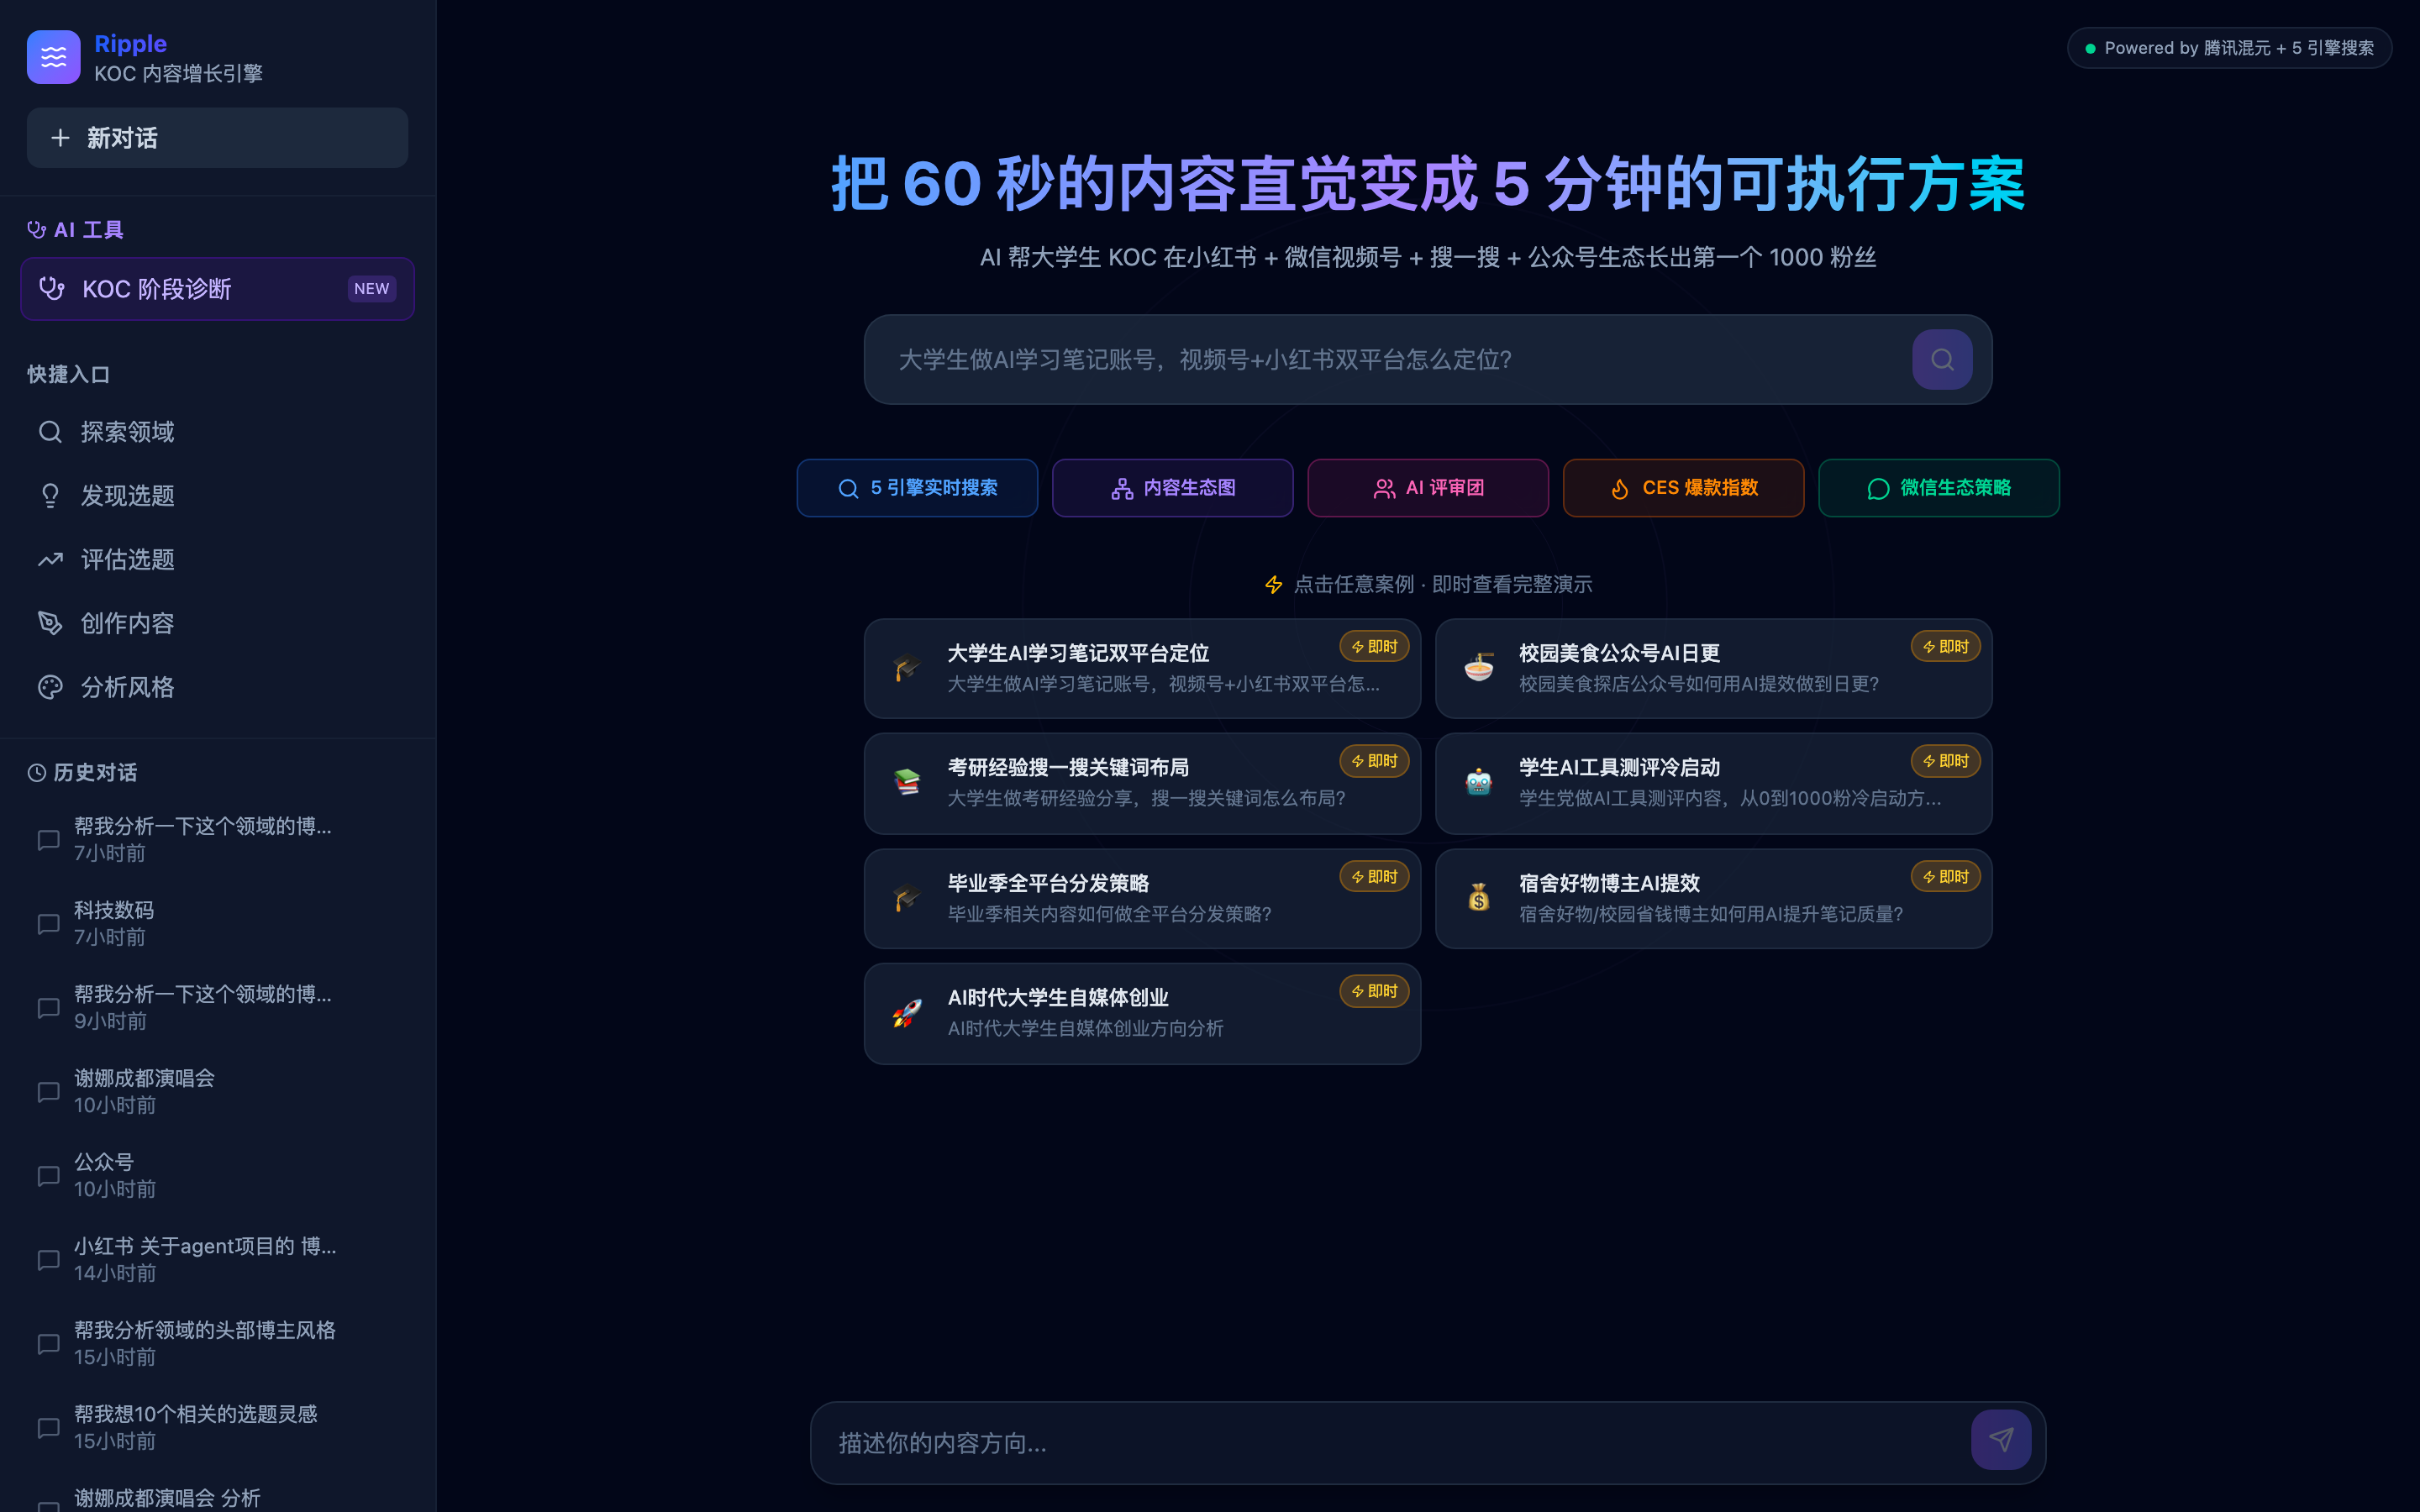
\includegraphics[width=14cm,keepaspectratio]{screenshots/hero.png}
\end{center}

\vspace{0.3cm}

\begin{center}
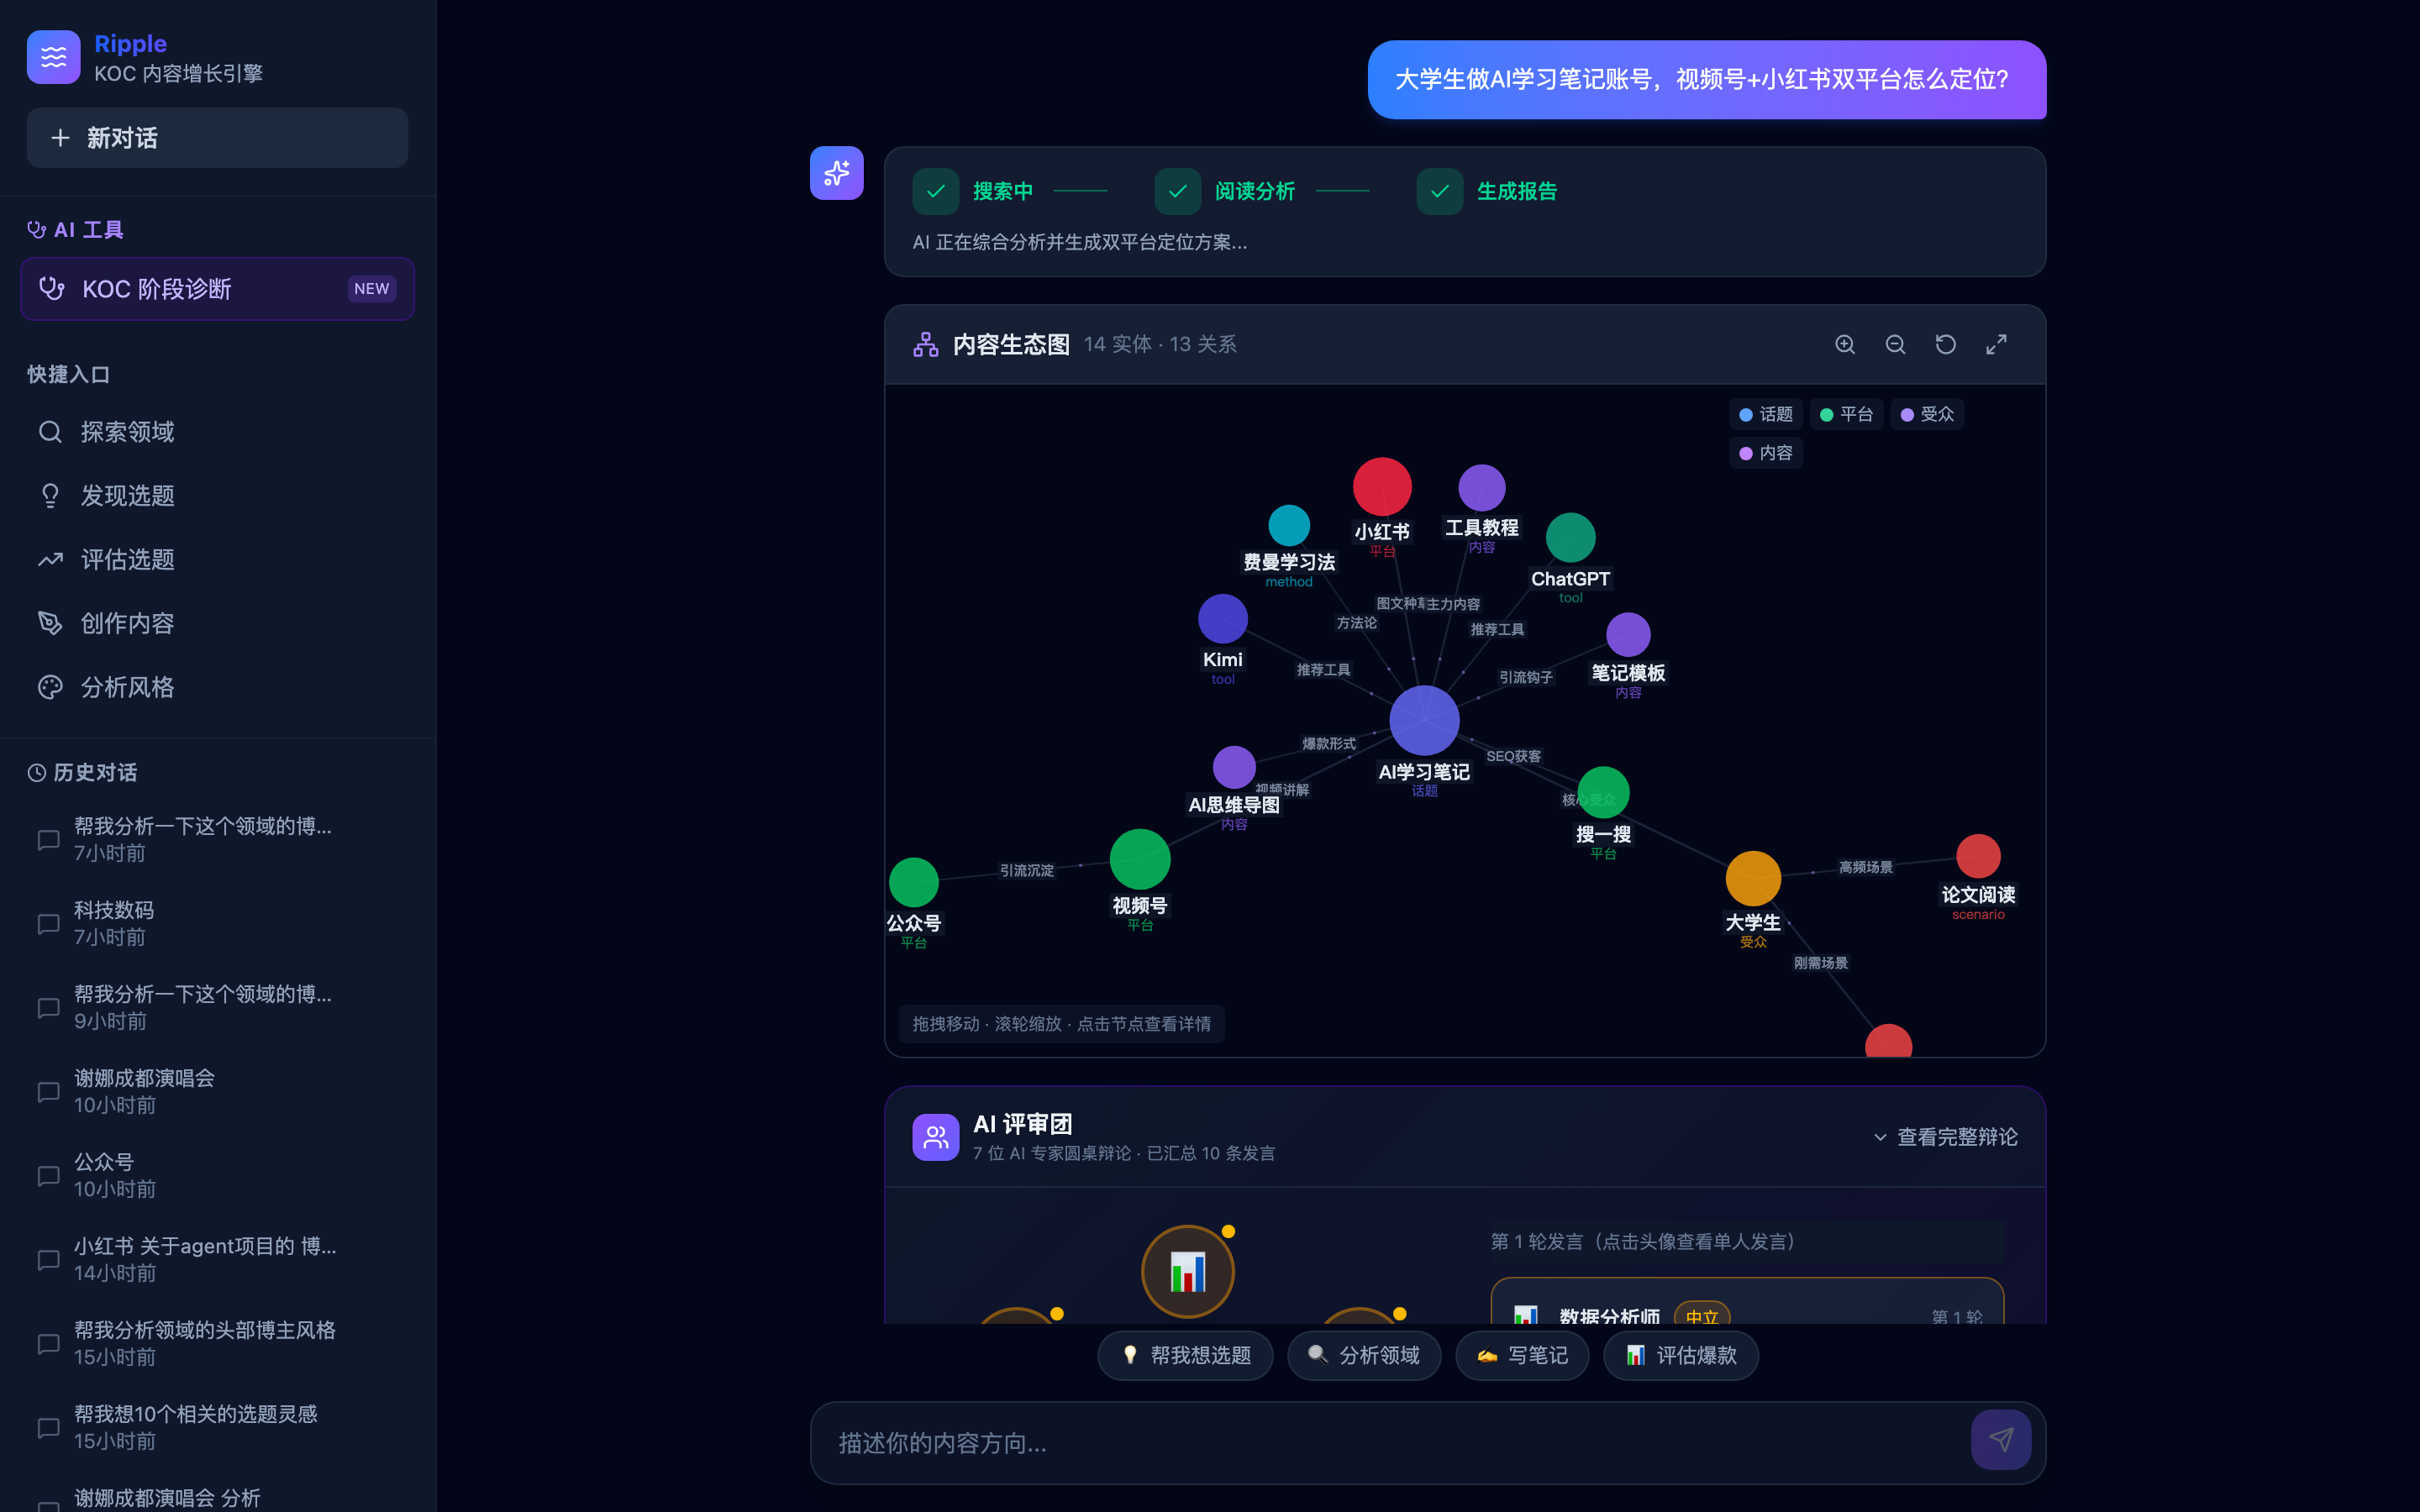
\includegraphics[width=14cm,keepaspectratio]{screenshots/content_eco.png}
\end{center}

\newpage

\begin{center}
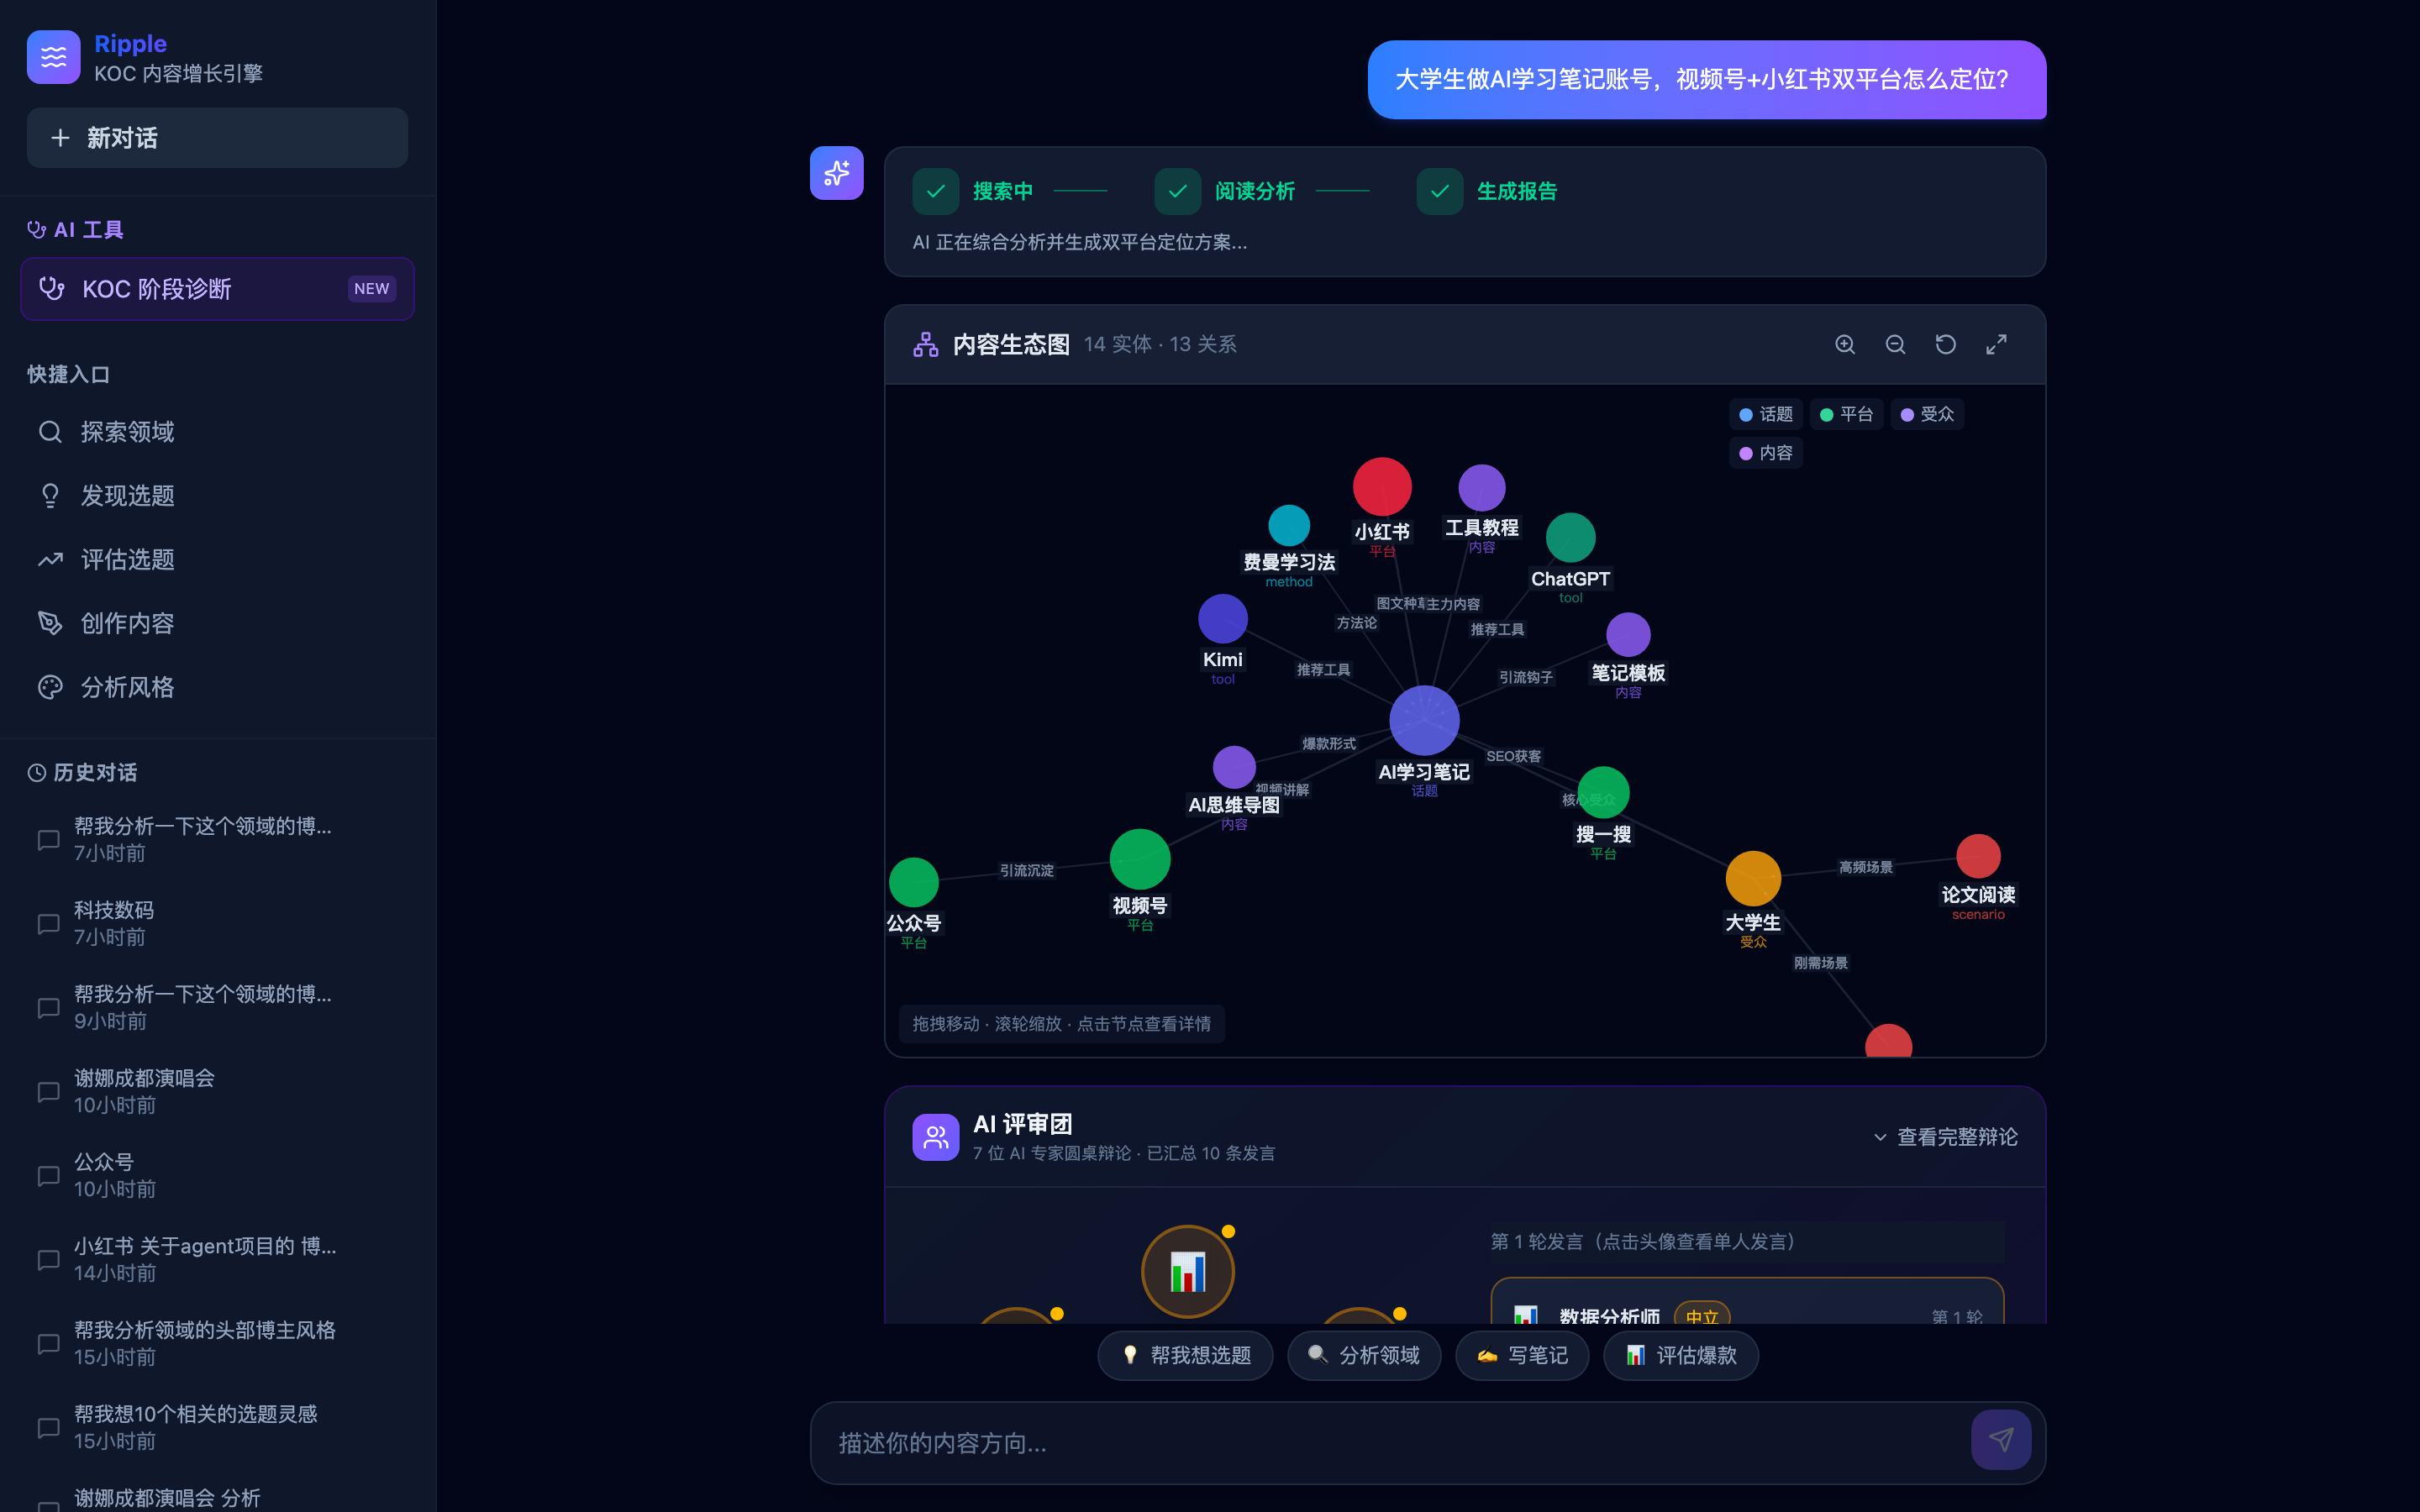
\includegraphics[width=14cm,keepaspectratio]{screenshots/roundtable.png}
\end{center}

\vspace{0.3cm}

\begin{center}
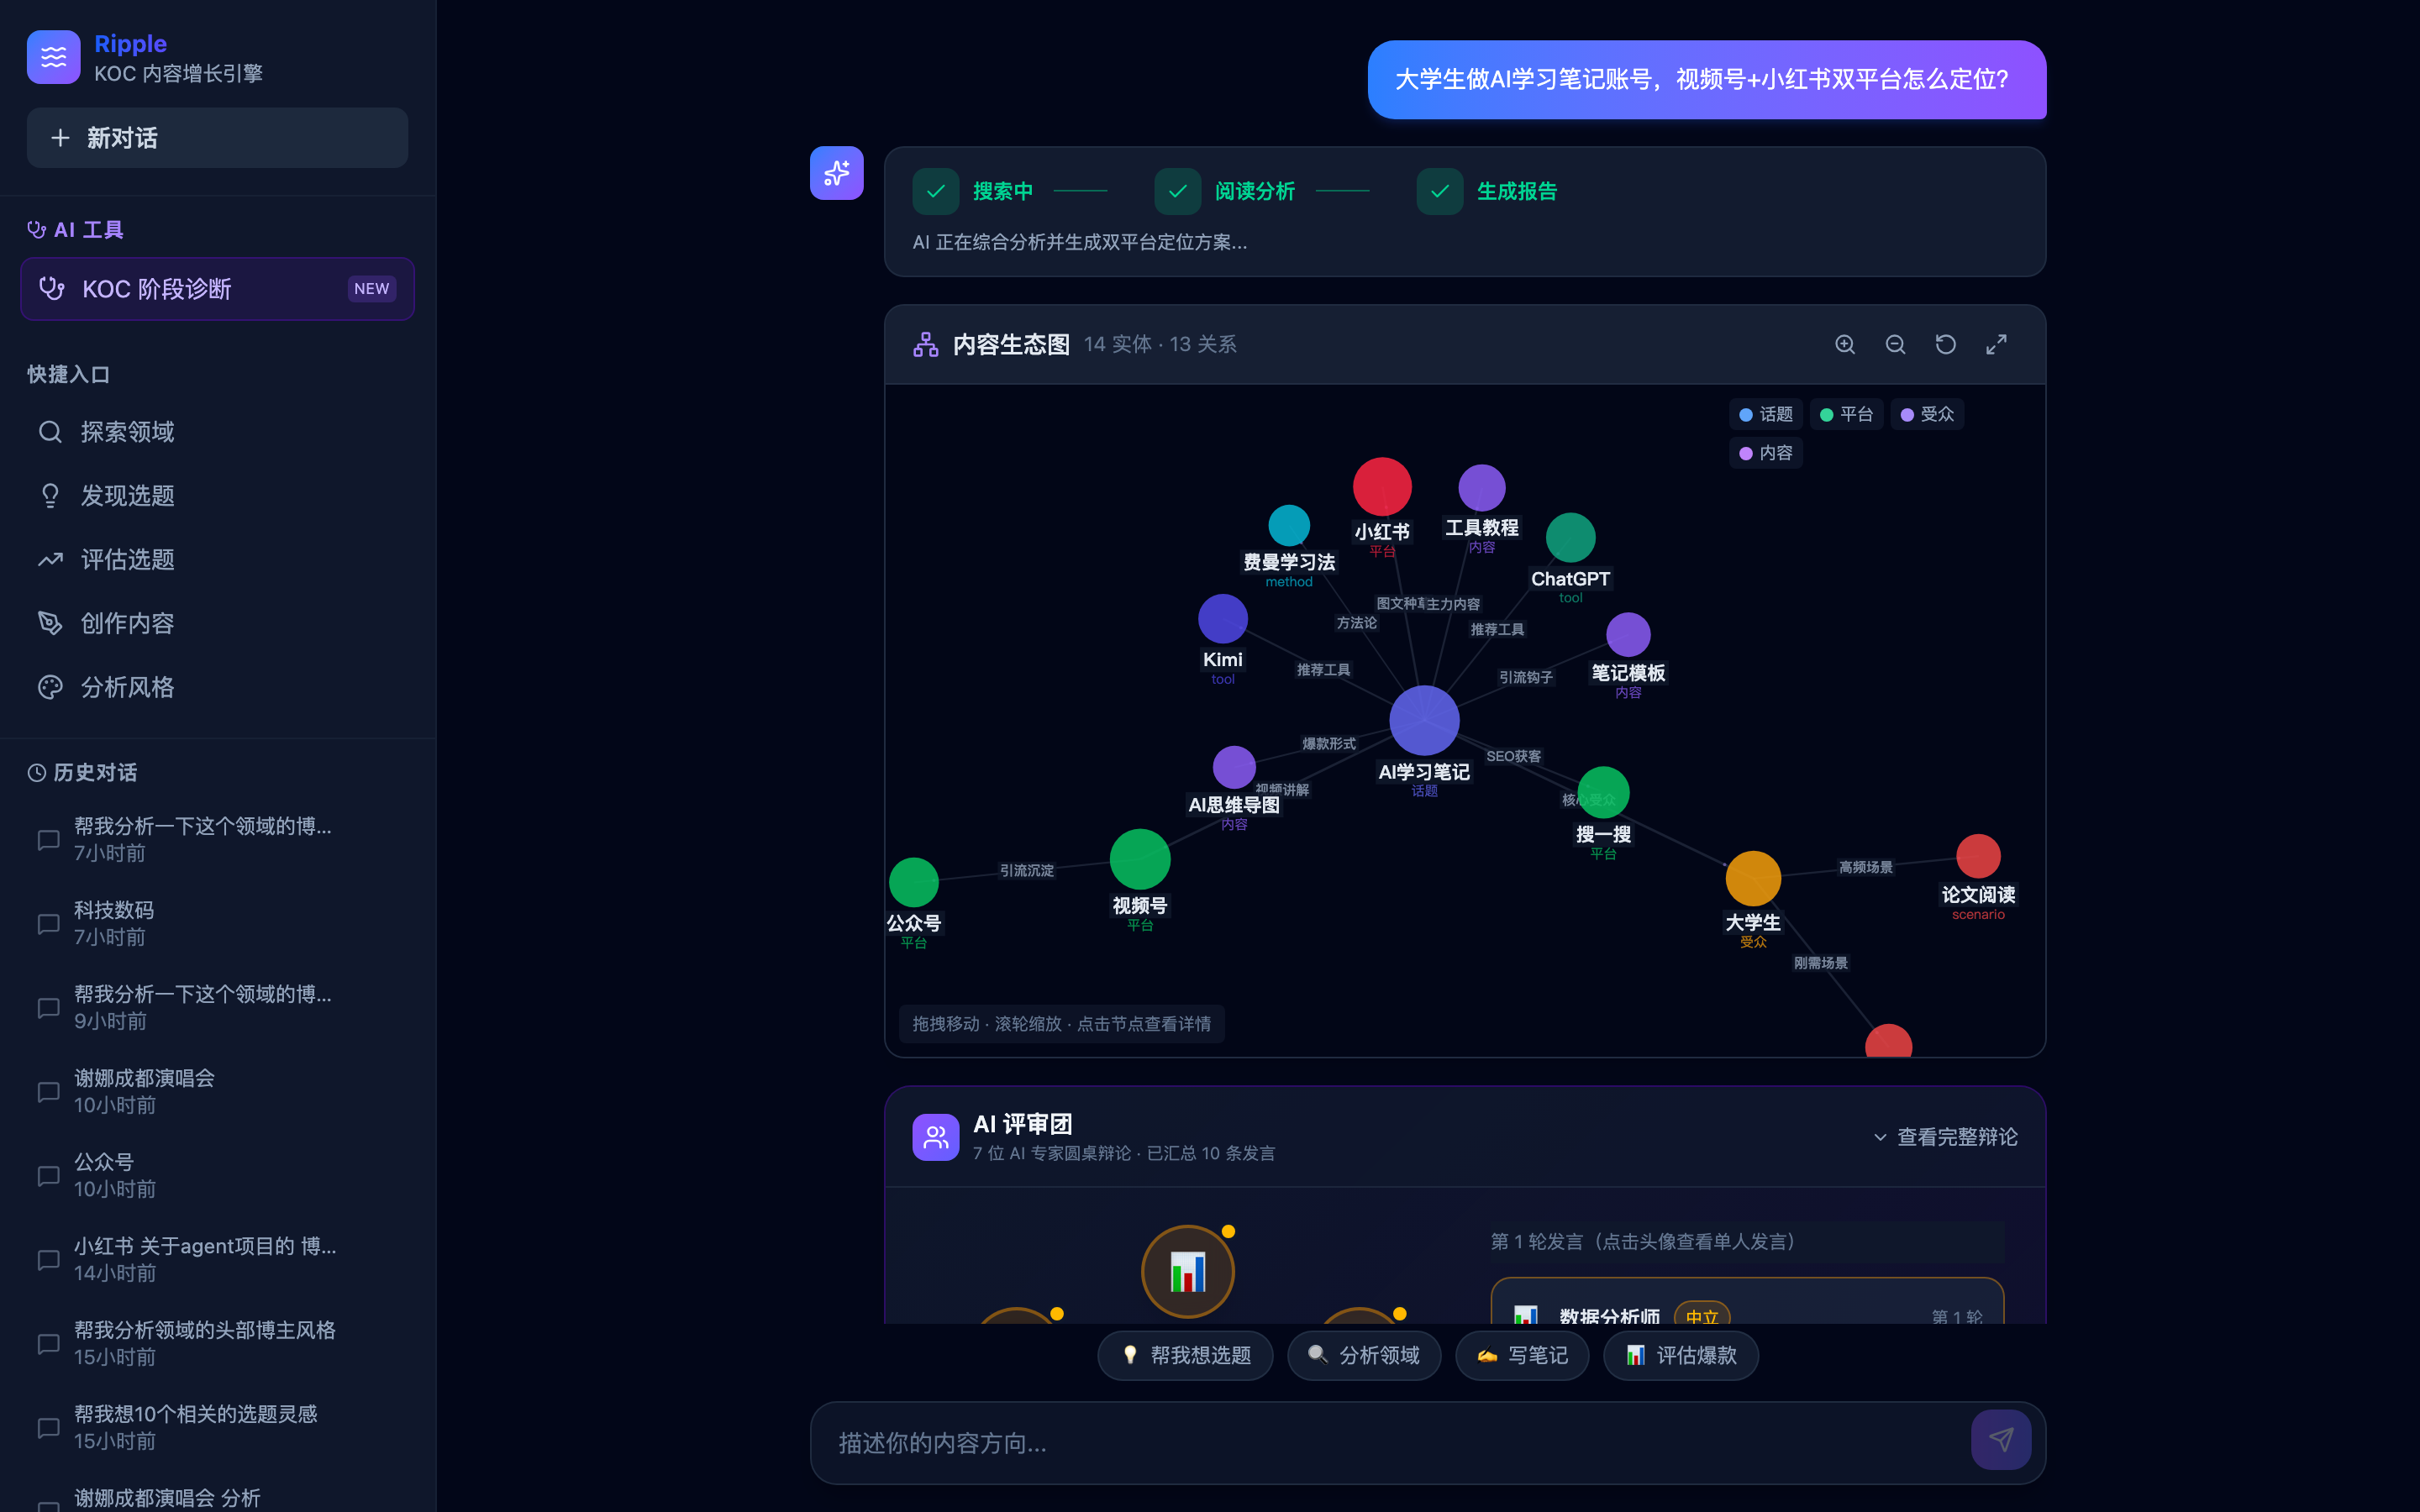
\includegraphics[width=14cm,keepaspectratio]{screenshots/ces_dash.png}
\end{center}

\newpage

\begin{center}
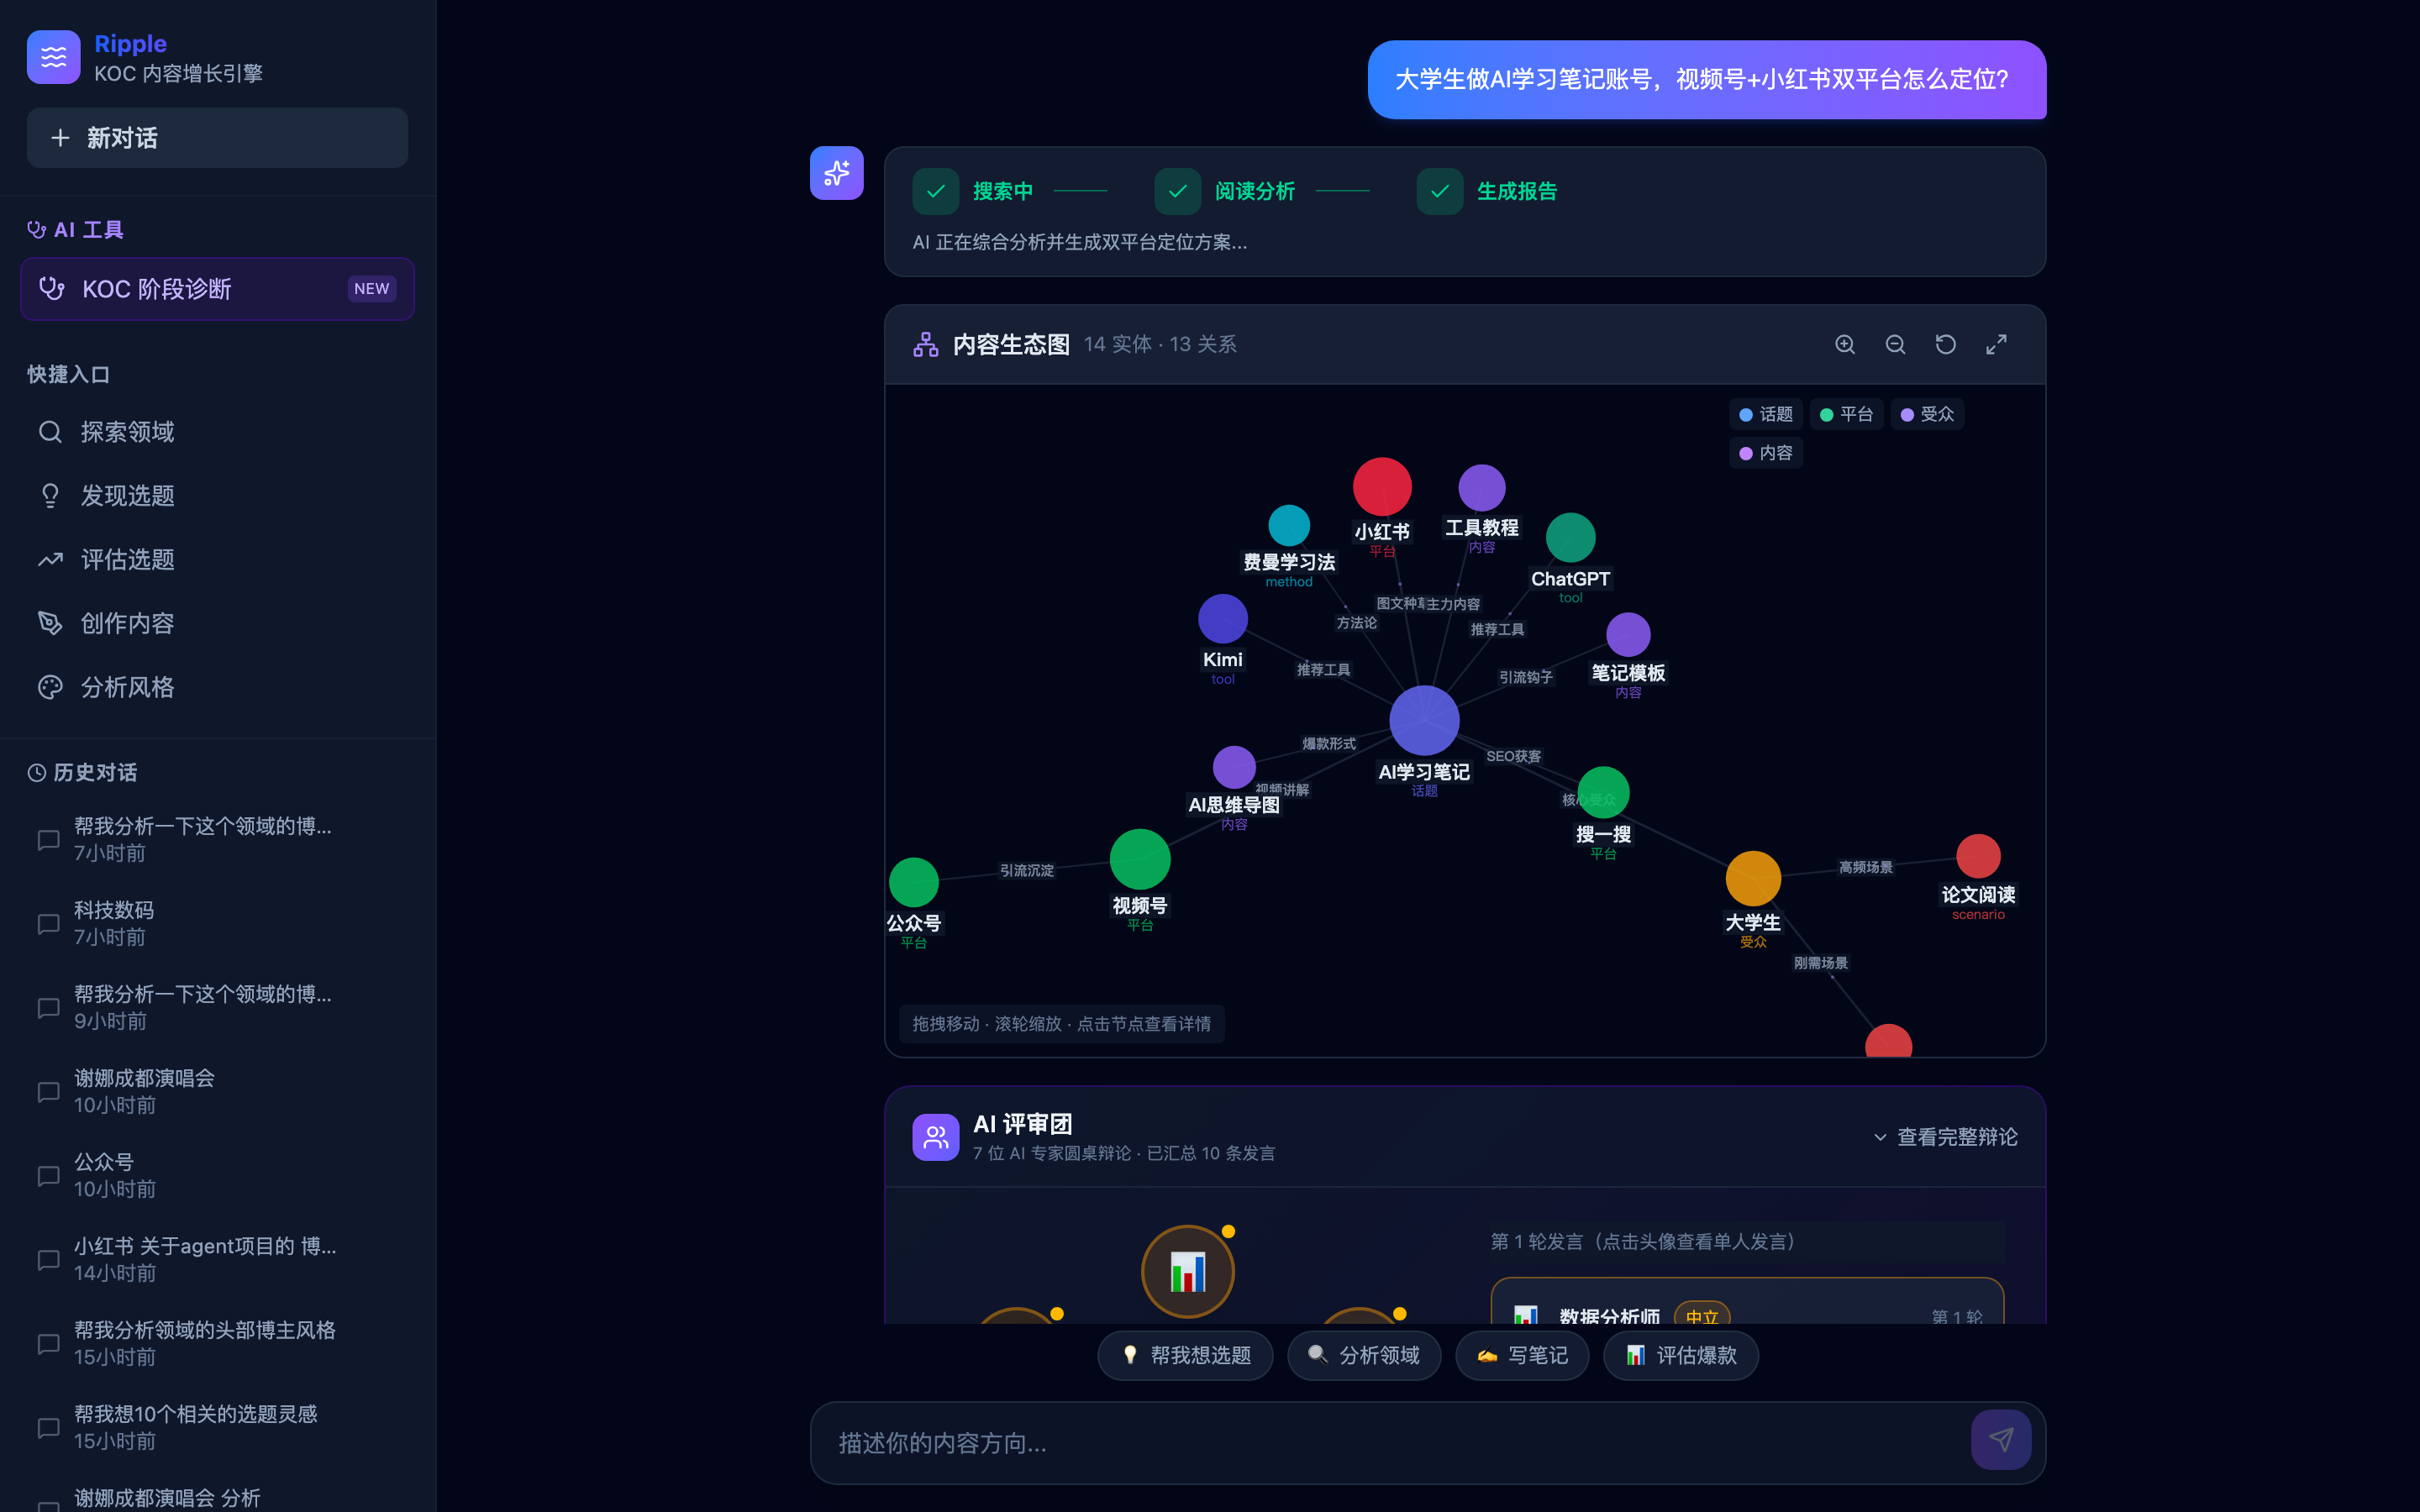
\includegraphics[width=14cm,keepaspectratio]{screenshots/koc_diagnose.png}
\end{center}

\vspace{0.3cm}

\begin{figure}[htbp]
\centering
\begin{subfigure}[b]{0.48\textwidth}
  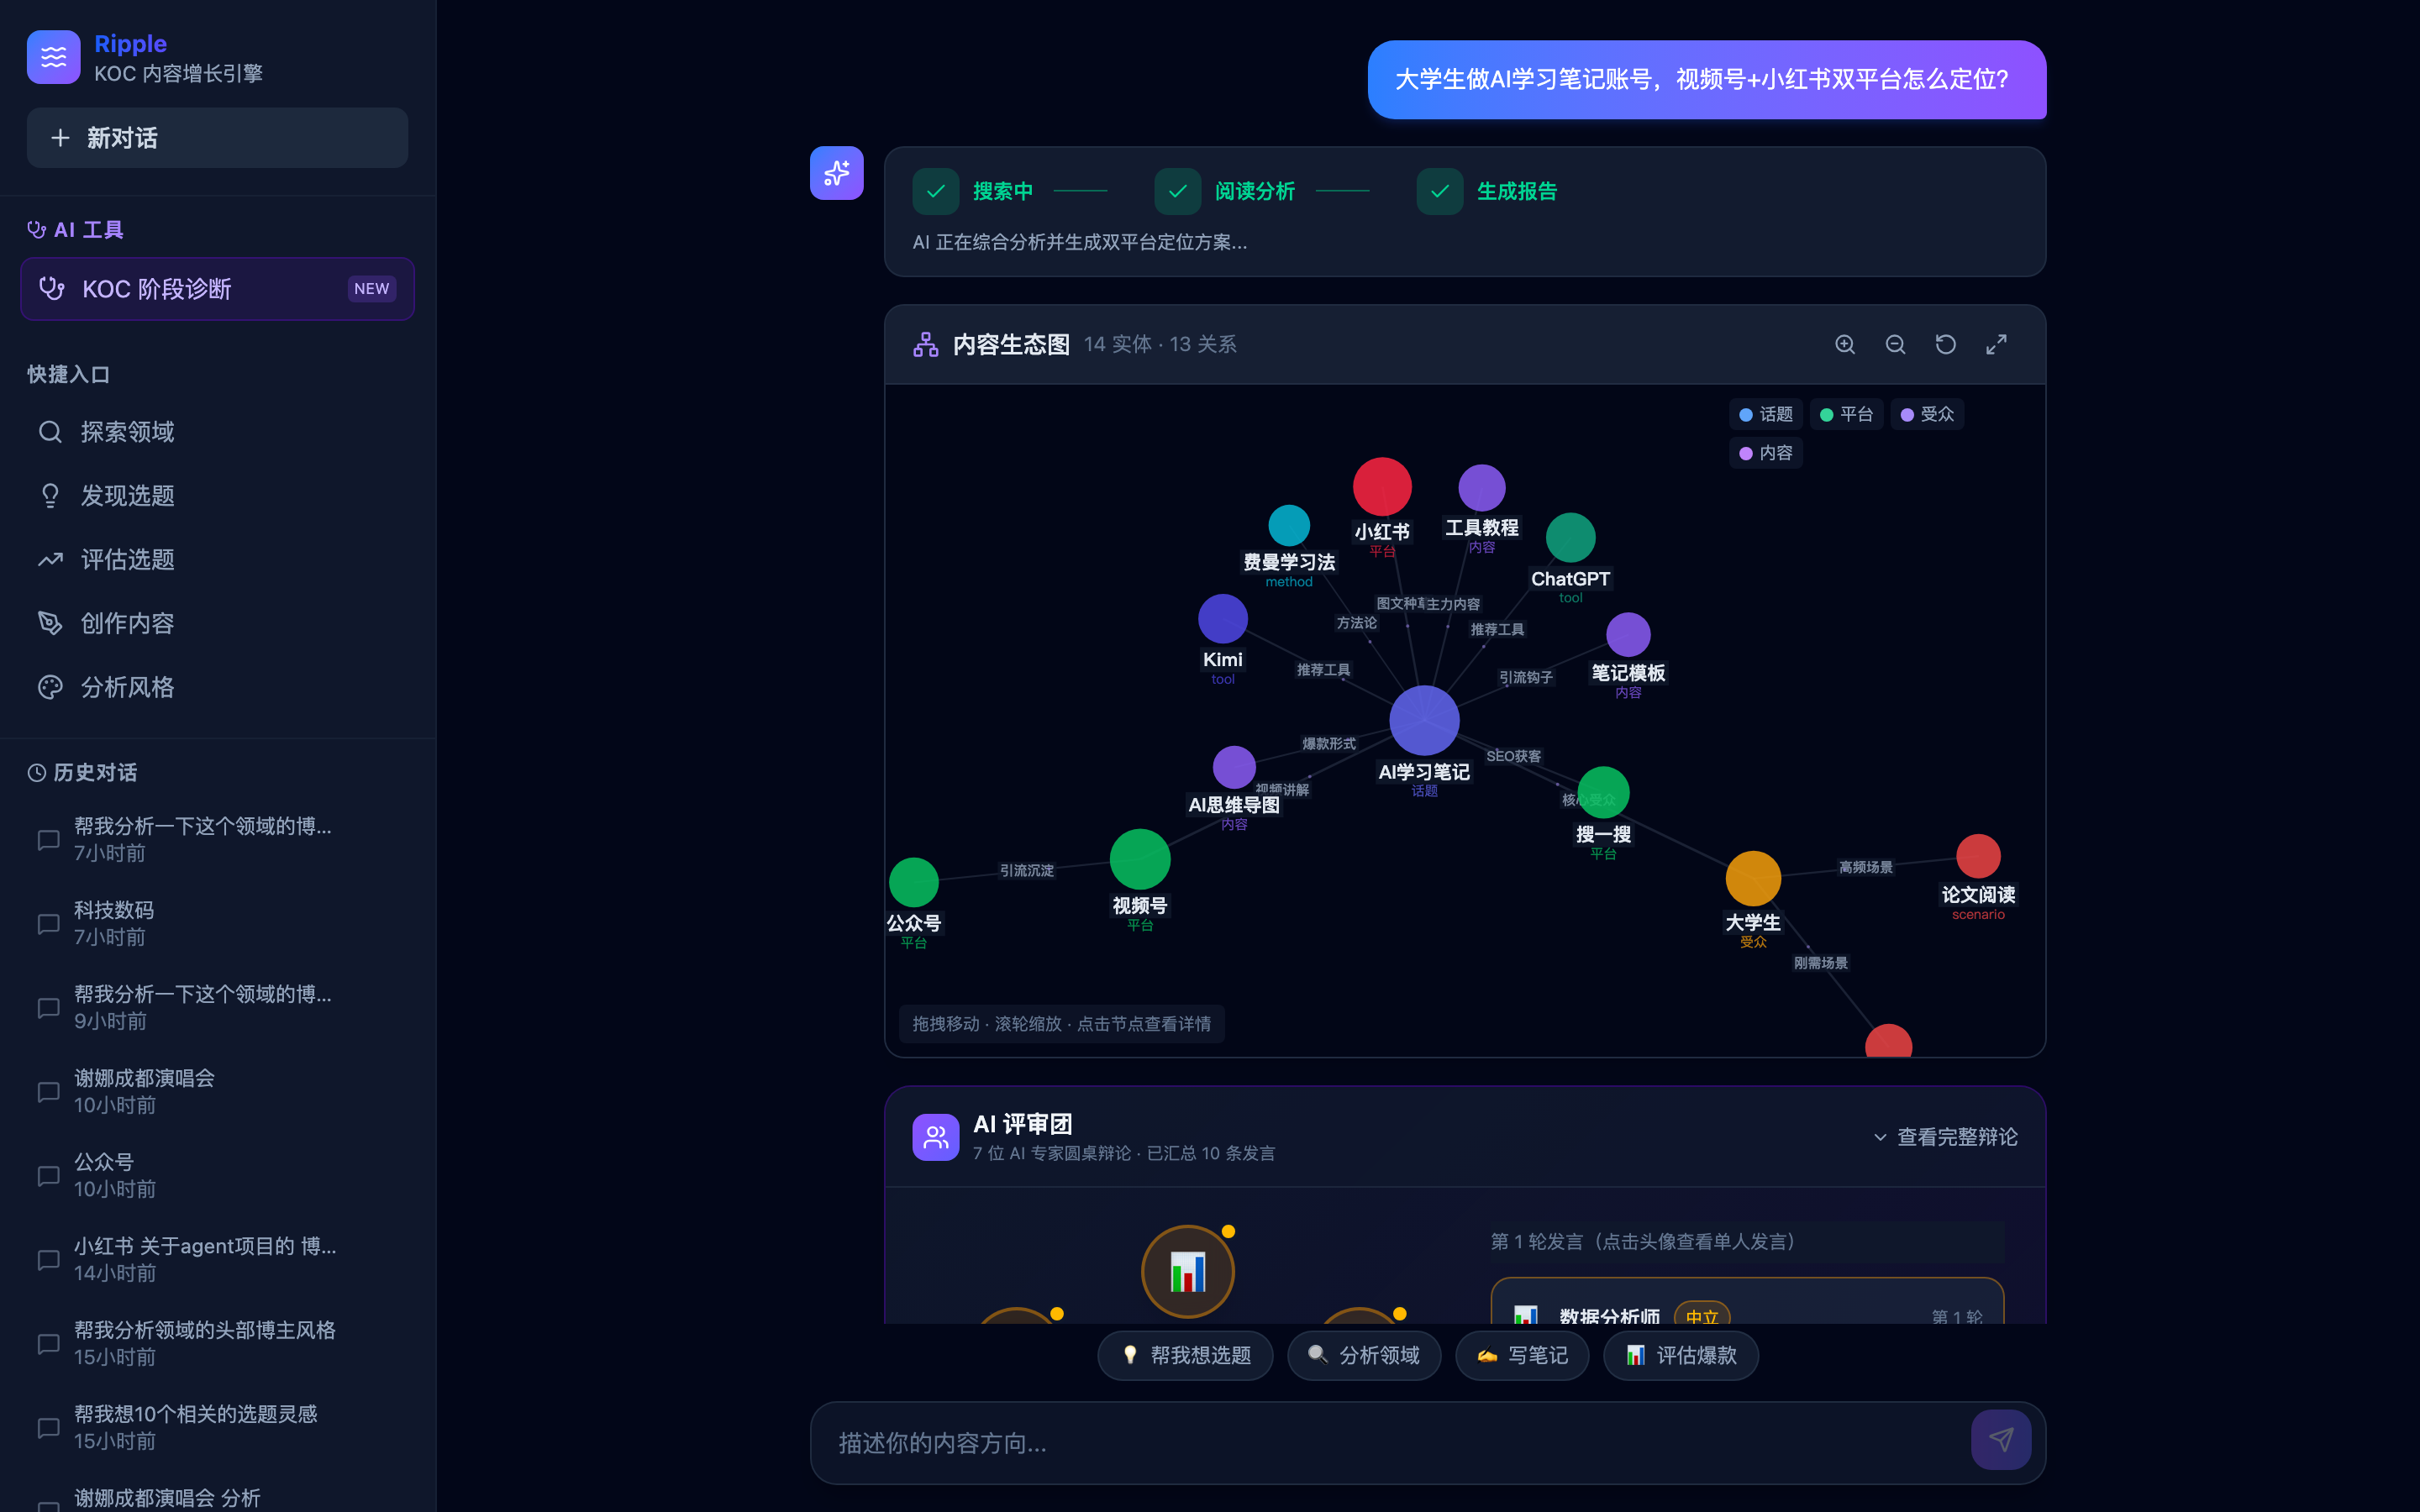
\includegraphics[width=6.5cm,keepaspectratio]{screenshots/wechat_search.png}
\end{subfigure}
\hfill
\begin{subfigure}[b]{0.48\textwidth}
  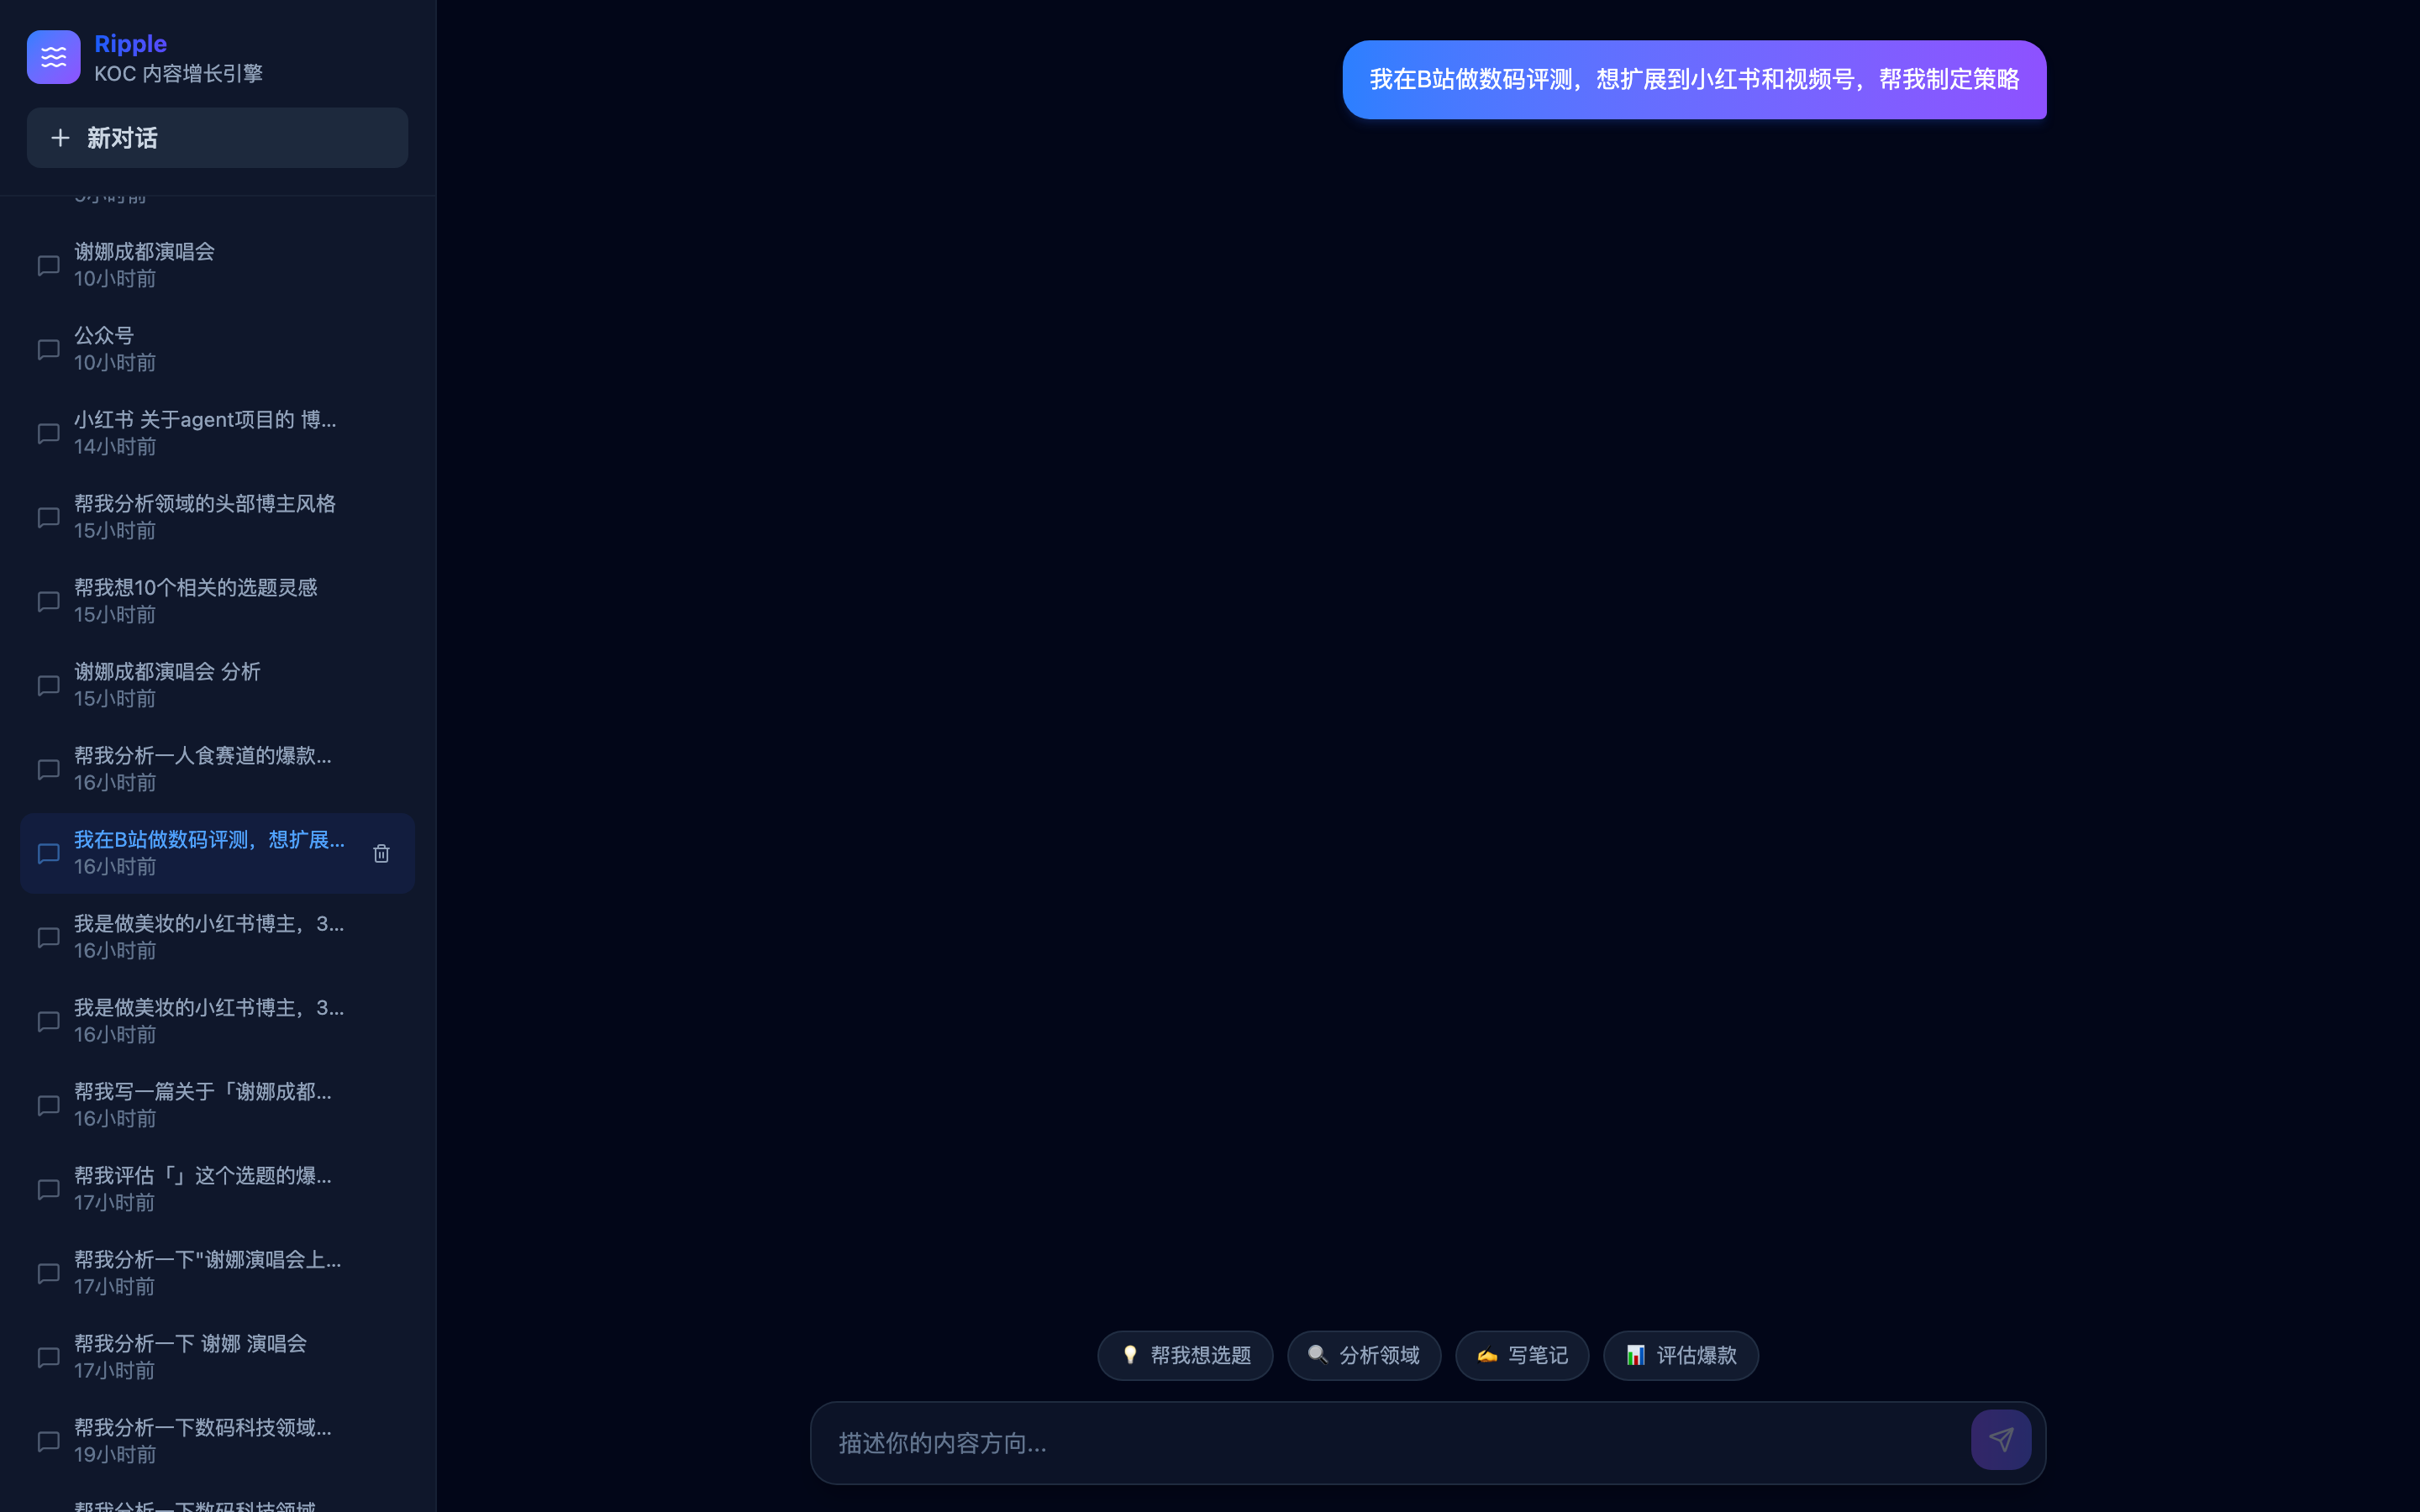
\includegraphics[width=6.5cm,keepaspectratio]{screenshots/wechat_video.png}
\end{subfigure}
\caption{微信生态面板}
\end{figure}

\begin{figure}[htbp]
\centering
\begin{subfigure}[b]{0.48\textwidth}
  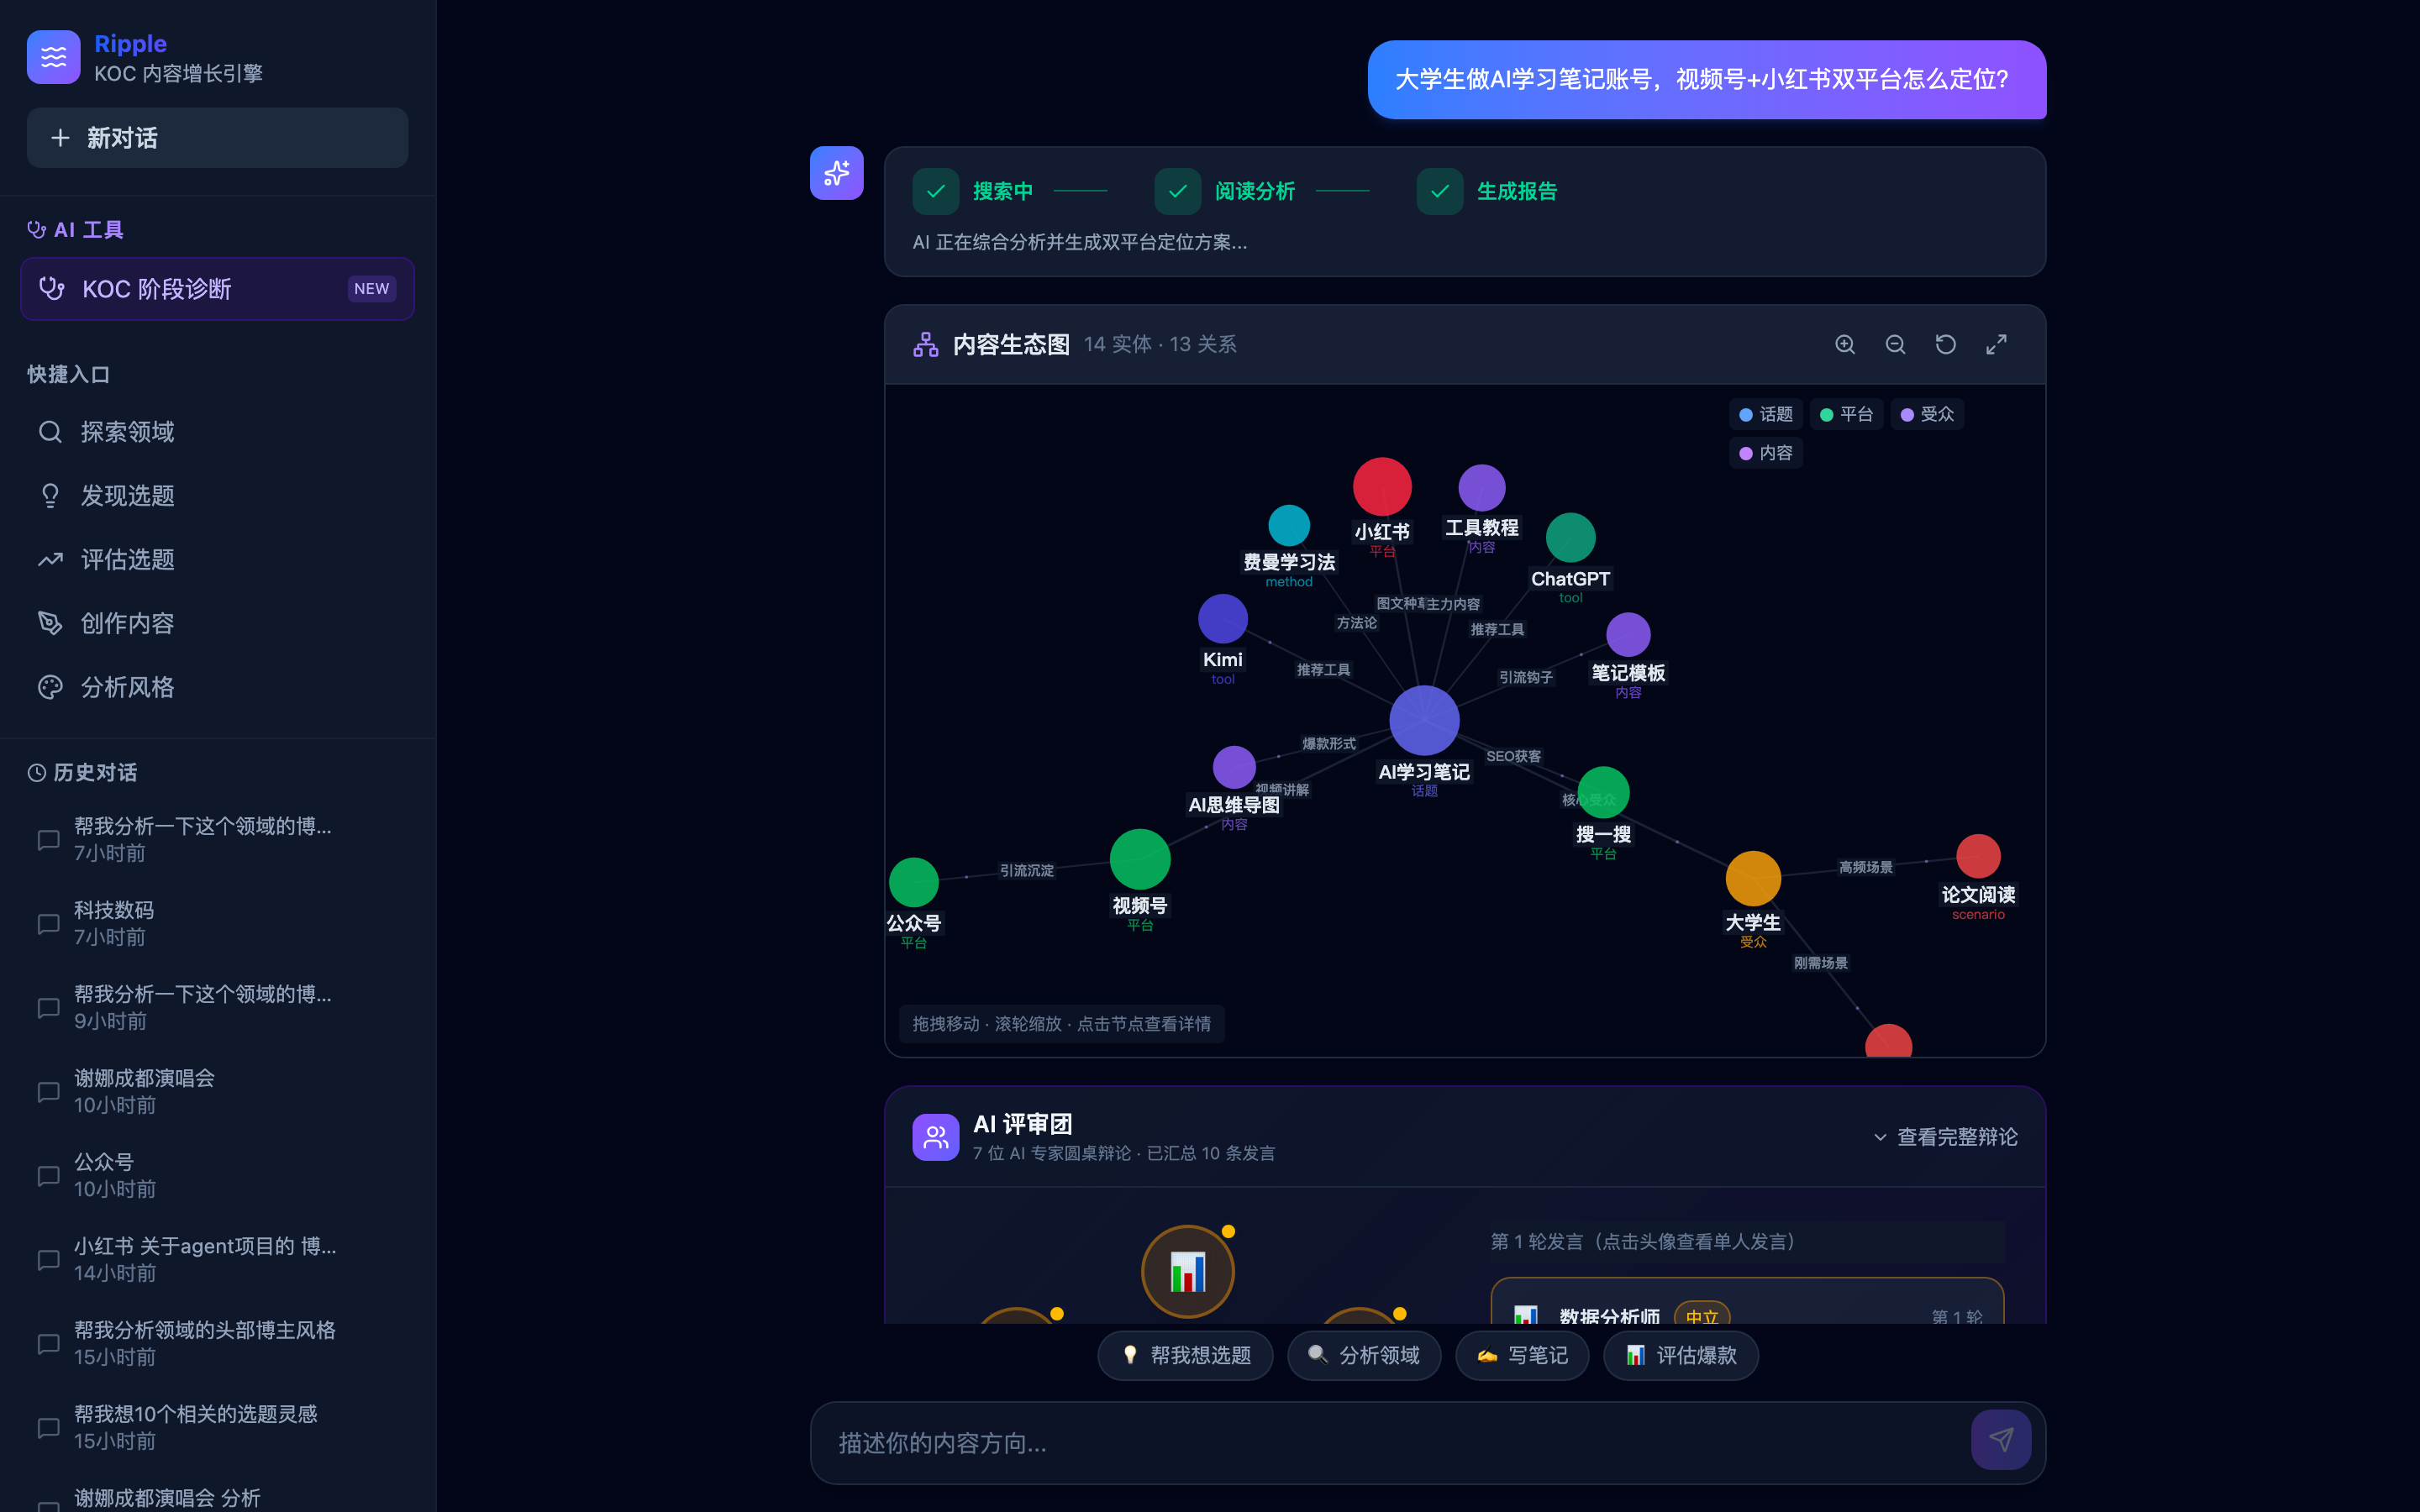
\includegraphics[width=6.5cm,keepaspectratio]{screenshots/ces_slider.png}
\end{subfigure}
\hfill
\begin{subfigure}[b]{0.48\textwidth}
  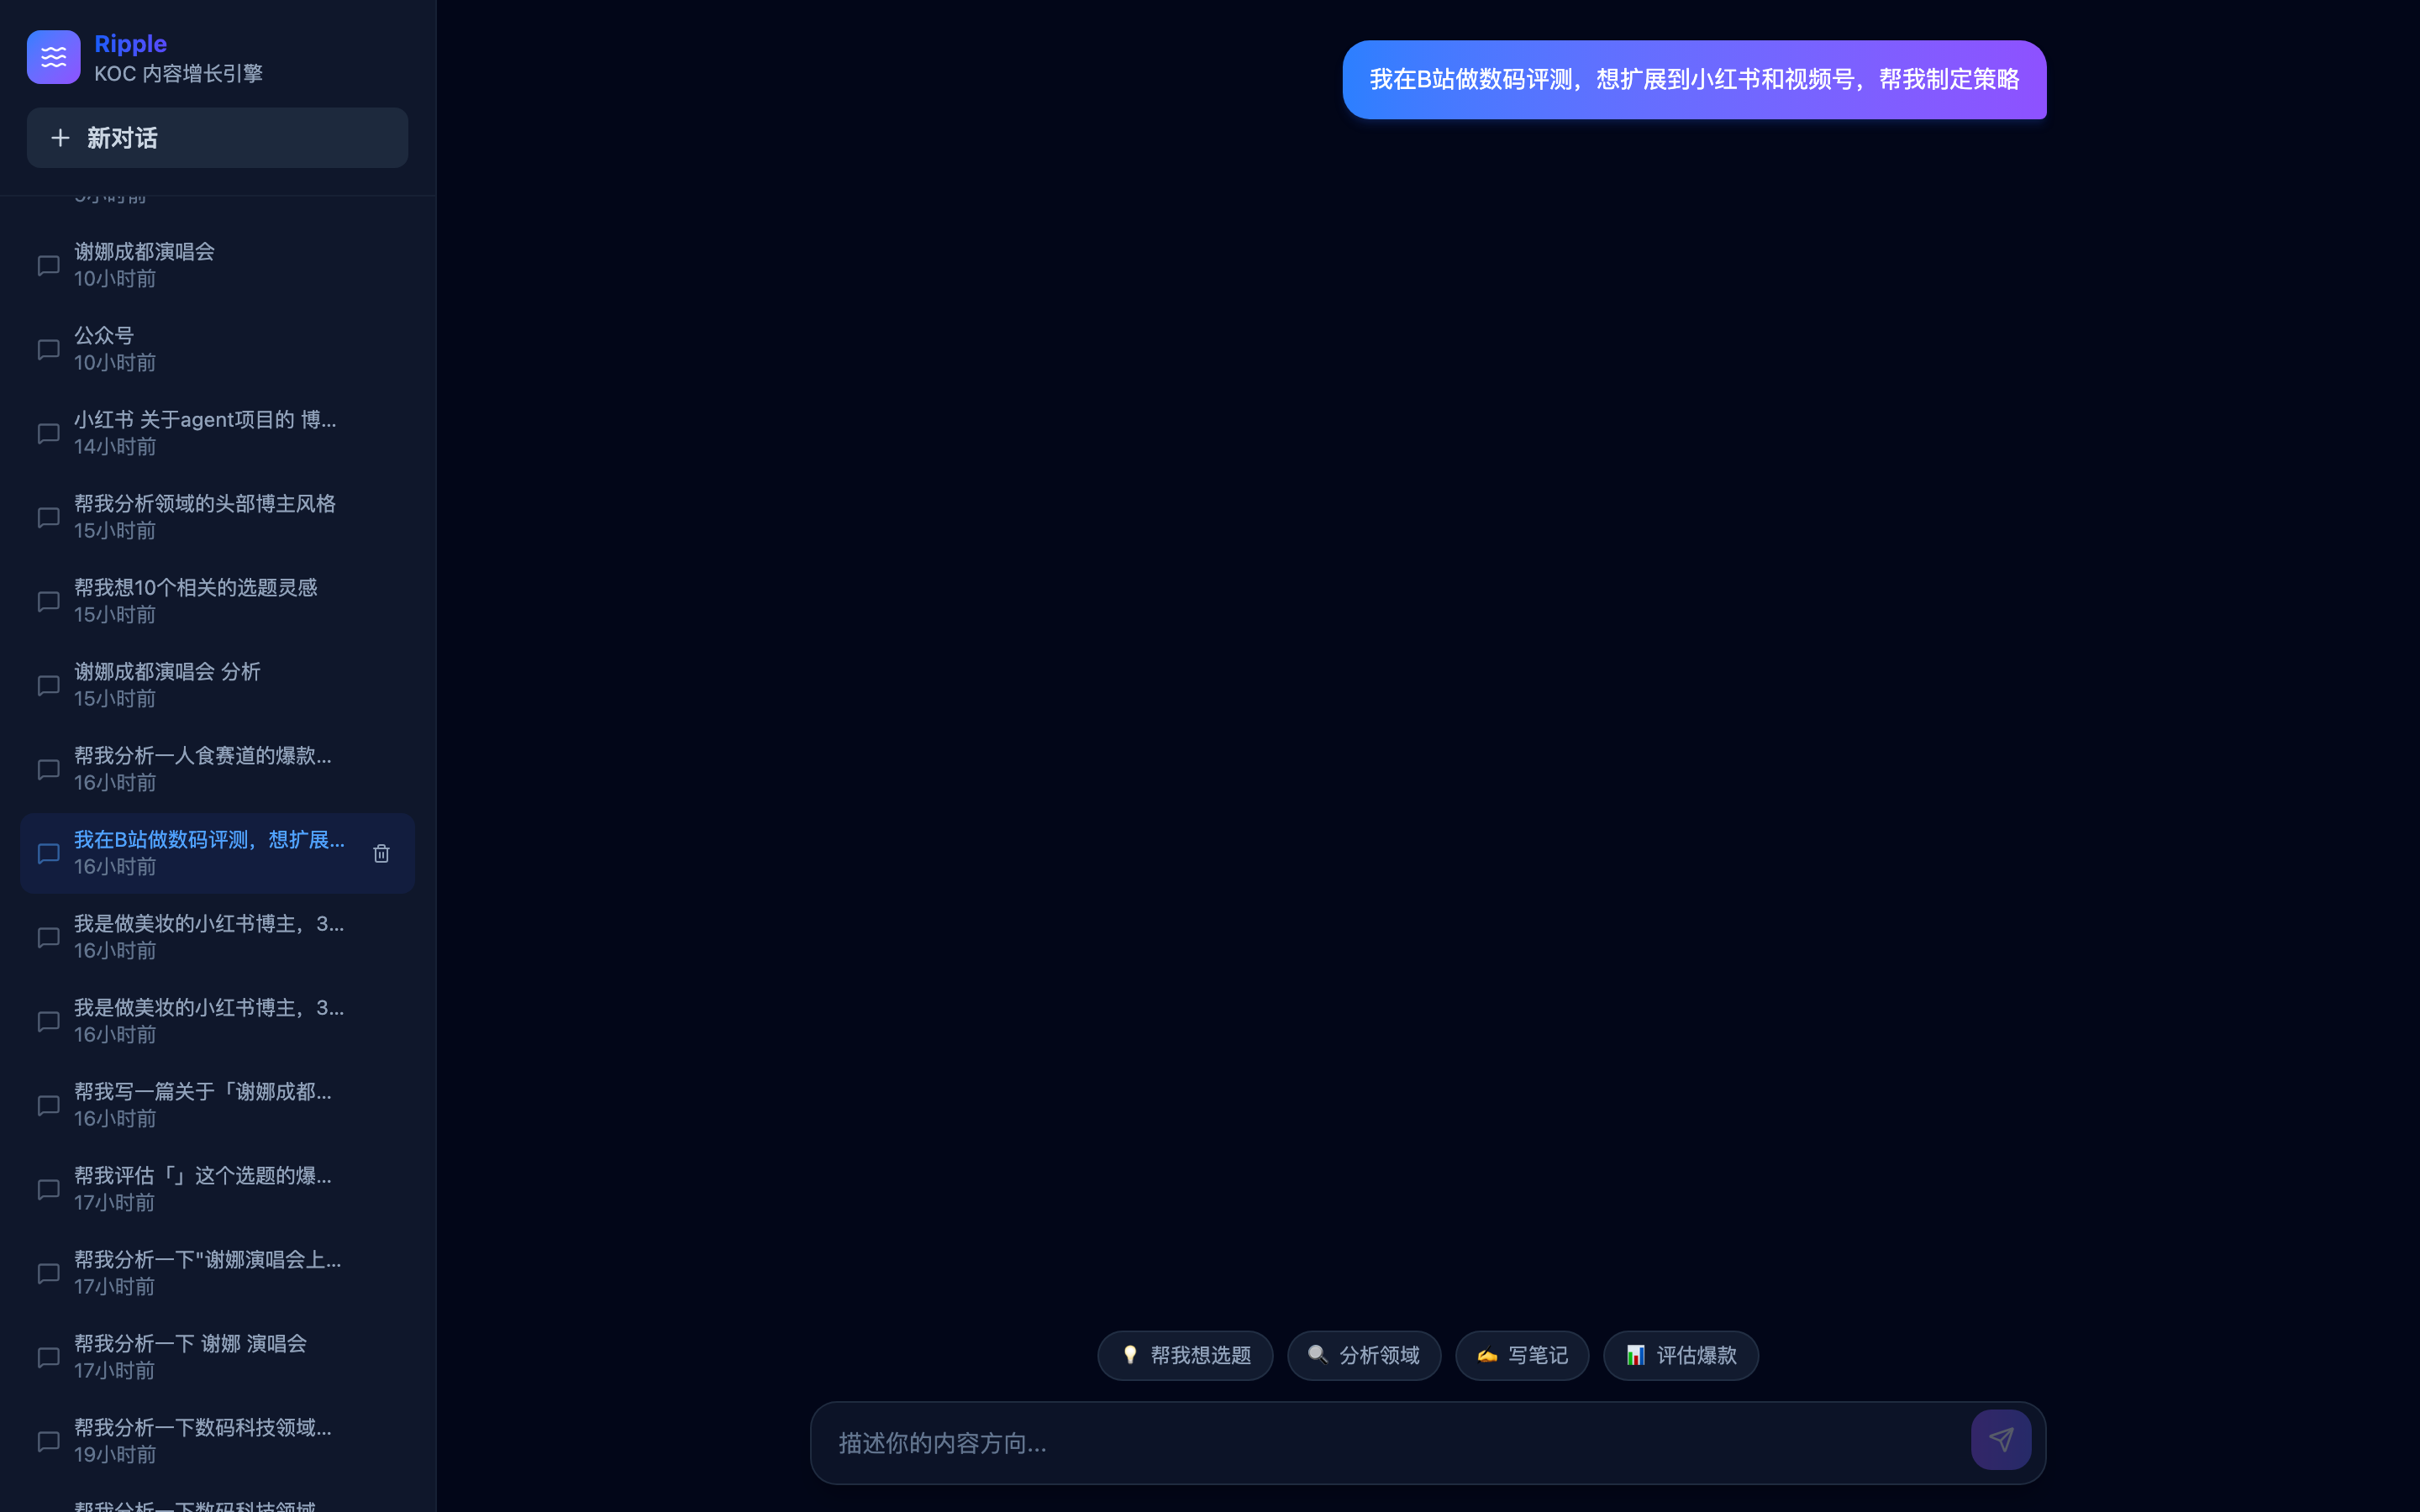
\includegraphics[width=6.5cm,keepaspectratio]{screenshots/copy_export.png}
\end{subfigure}
\caption{CES 模拟器交互 + 多平台导出}
\end{figure}

\newpage

\begin{center}
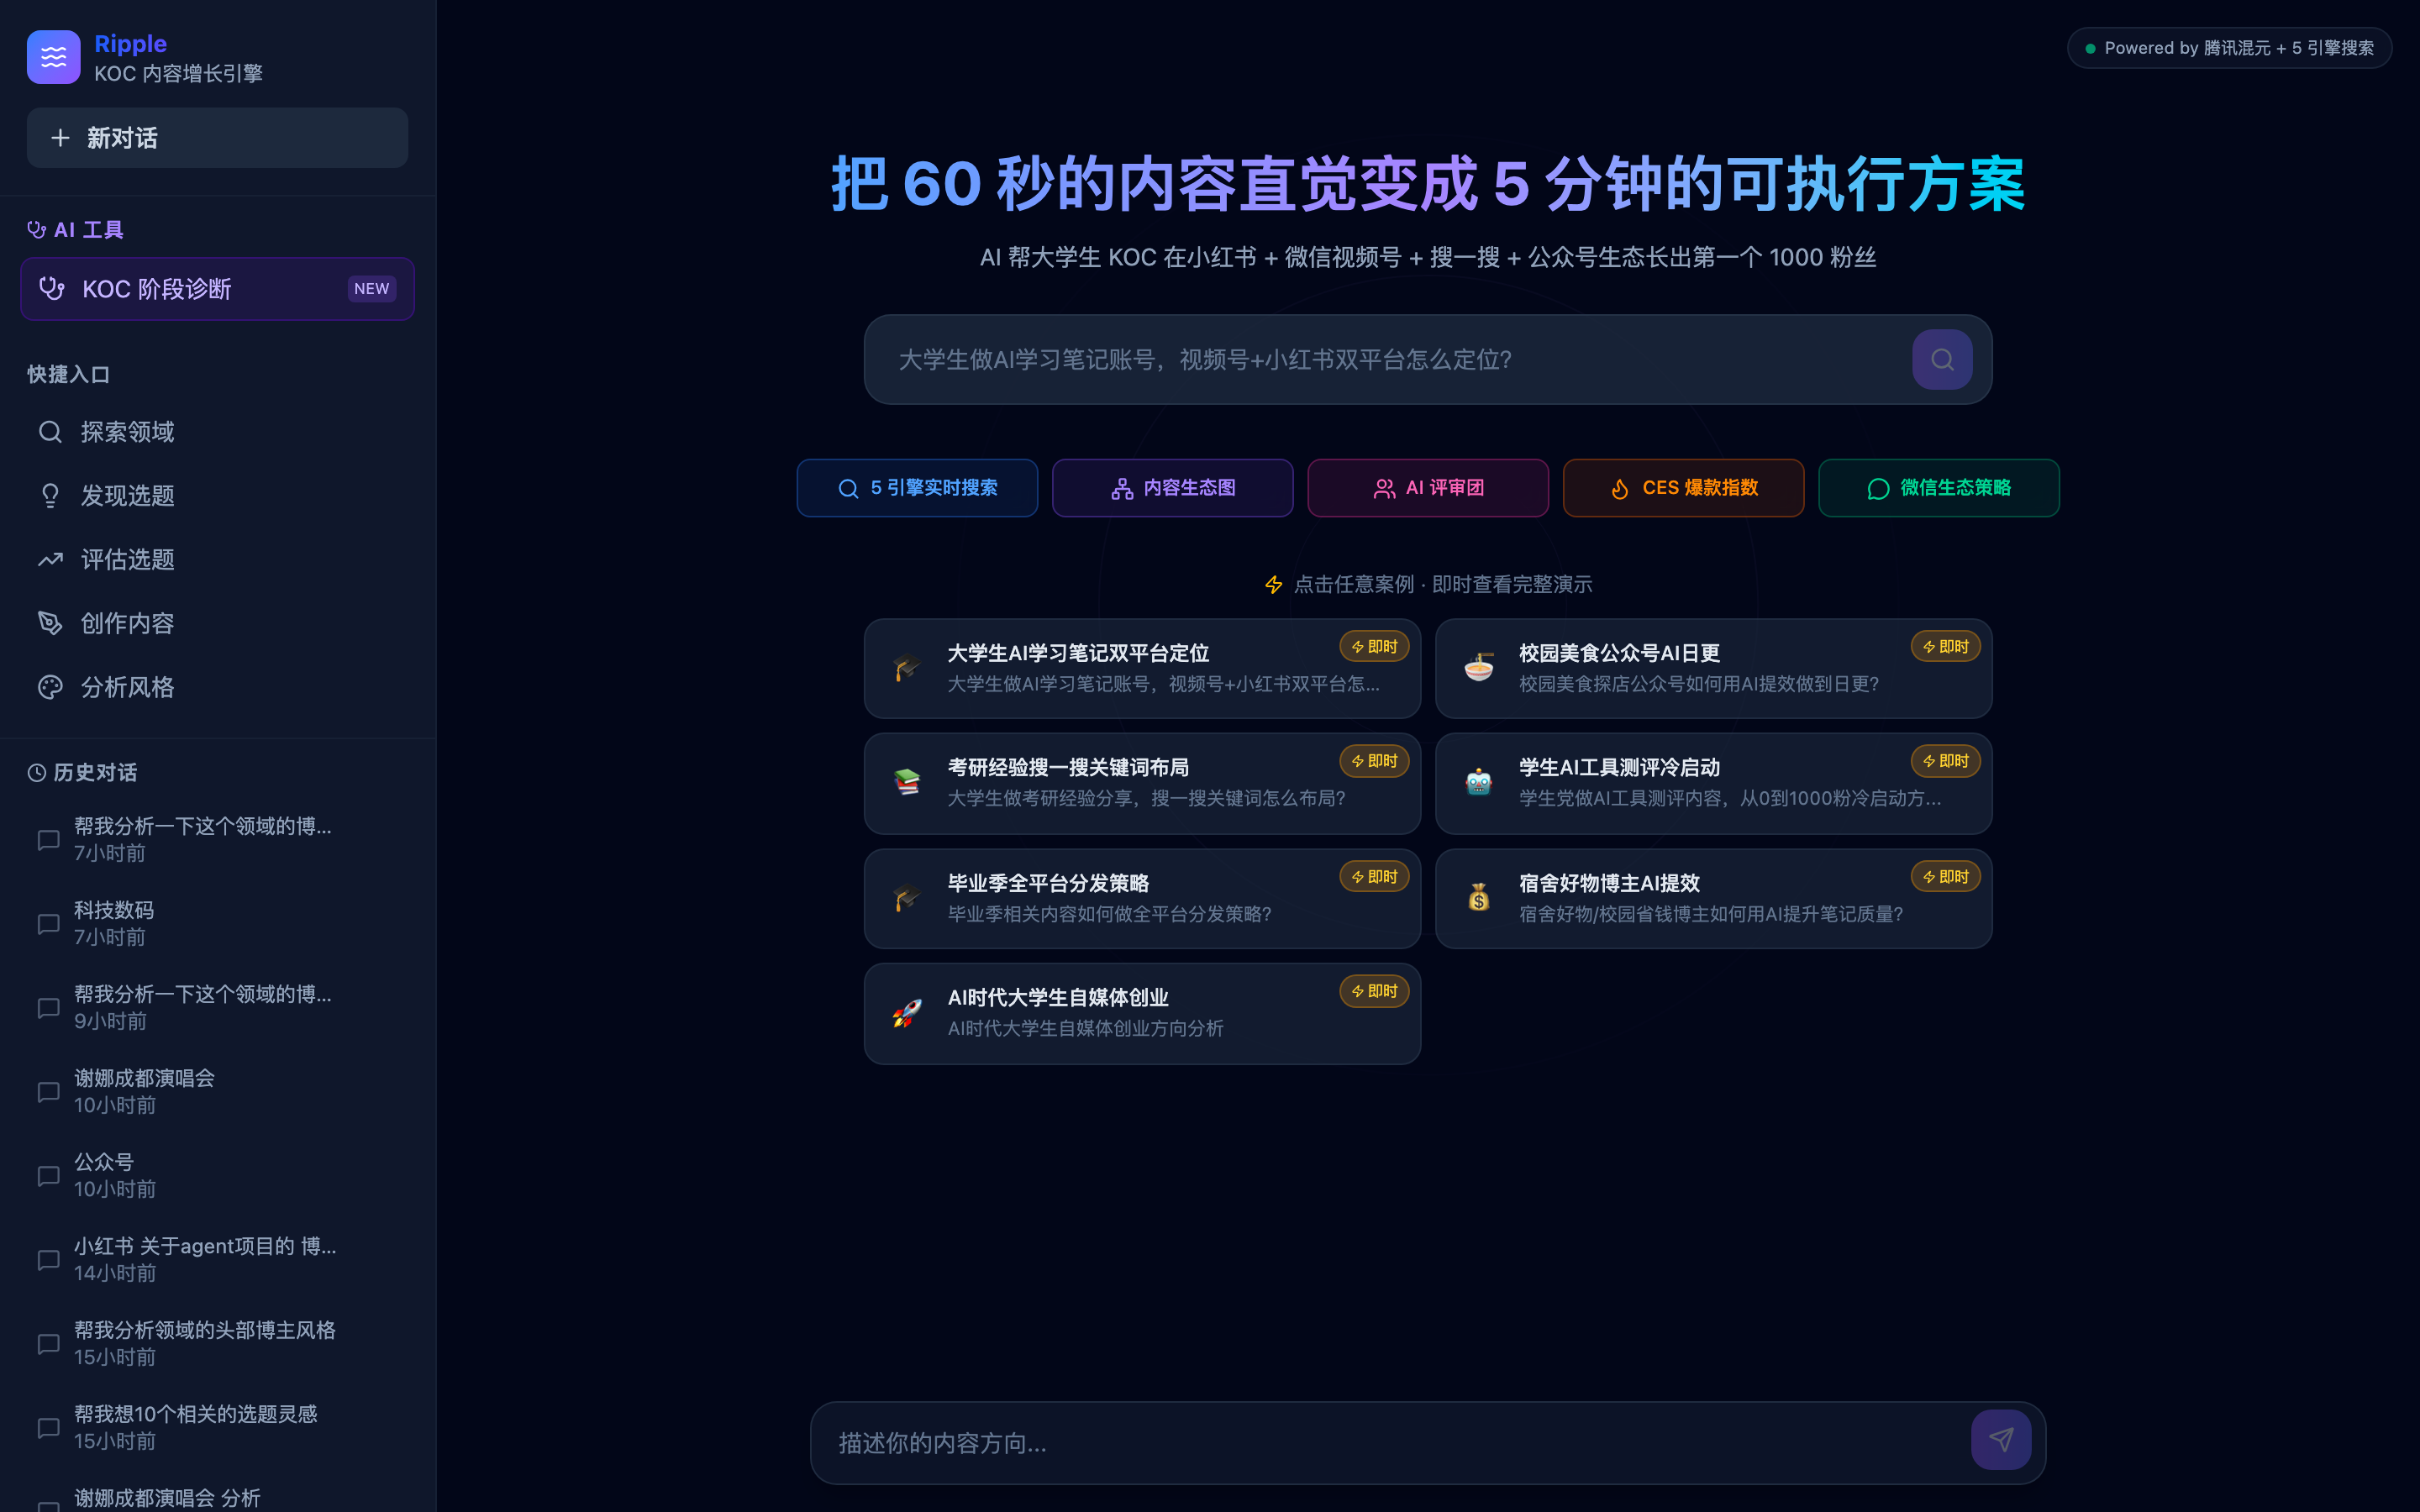
\includegraphics[width=14cm,keepaspectratio]{screenshots/demo_cases.png}
\end{center}


\section{关键数据指标一览}

\begin{center}
\begin{tabular}{p{5cm} p{3cm} p{5cm}}
\toprule
\textbf{指标} & \textbf{数据} & \textbf{说明} \\
\midrule
Demo 响应时间 & $<$1 秒 & 完整 Mock 数据预缓存，零延迟体验 \\[2pt]
图谱生成时间 & 8-12 秒 & Single-Pass 优化后 \\[2pt]
7 Agent 并行耗时 & 15-20 秒 & asyncio.gather 并行调度 \\[2pt]
CES 评分维度 & 19 维 & 覆盖所有影响传播的关键因素 \\[2pt]
搜索引擎数量 & 5 个 & 全域搜索矩阵 \\[2pt]
支持平台数量 & 4 个 & 小红书/视频号/公众号/抖音 \\[2pt]
Demo 案例数量 & 6 个 & 覆盖 6 大学生 KOC 典型场景 \\[2pt]
一键导出格式 & 4 种 & 小红书/视频号脚本/公众号/原文 \\[2pt]
前端组件数量 & 30+ & React 组件，TypeScript 严格模式 \\[2pt]
前端代码行数 & $\sim$8,000 行 & TypeScript + TSX \\[2pt]
后端代码行数 & $\sim$4,500 行 & Python + FastAPI \\
\bottomrule
\end{tabular}
\end{center}


% ============================================================
%  PART 6  团队介绍
% ============================================================
\newpage
\section{团队介绍}

\subsection{作者：戴尚好}

\begin{tcolorbox}[colback=primary!5,colframe=primary,arc=6pt,
  left=12pt,right=12pt,top=10pt,bottom=10pt]
\begin{tabular}{p{4cm} p{10cm}}
\textbf{姓名} & 戴尚好 \\[4pt]
\textbf{院校} & 中国科学技术大学（在读硕士）\\[4pt]
\textbf{本科} & 山东大学 \\[4pt]
\textbf{邮箱} & \href{mailto:bcefghj@163.com}{bcefghj@163.com} \\[4pt]
\textbf{手机} & 13296886603 \\[4pt]
\textbf{主页} & \url{https://bcefghj.github.io/} \\[4pt]
\textbf{GitHub} & \url{https://github.com/bcefghj} \\[4pt]
\textbf{小红书} & @bcefghj（1.6 万粉丝）\\
\end{tabular}
\end{tcolorbox}

\subsection{技术背景}

\textbf{研究论文：}

Nature Computational Science 一作论文（IF = 18），
在全球顶级综合性科学期刊发表计算科学研究成果，
体现了从学术研究到工程实践的跨越能力。

\textbf{竞赛荣誉：}

\begin{itemize}
  \item 全国大学生数学竞赛一等奖
  \item 山东大学学业奖学金一等奖
  \item 中国科学技术大学学业奖学金一等奖
\end{itemize}

\textbf{开源影响力（GitHub）：}

\begin{center}
\begin{tabular}{p{4cm} p{3cm} p{6cm}}
\toprule
\textbf{项目} & \textbf{Stars} & \textbf{描述} \\
\midrule
Claude Code 源码分析 & 301 & 51 万行 TypeScript 源码逆向分析 \\[2pt]
AI Agent 面试全攻略 & 285 & 200+ 面试题 + 三语言企业级项目 \\[2pt]
多 Agent 电商推荐系统 & 66 & Supervisor 编排 + Redis + A/B Testing \\[2pt]
Learn Nanobot Agent & 68 & 17 章深度教程 + 134 道八股文 \\[2pt]
miniClaudeCode 框架 & 52 & Claude Code 核心架构 $\sim$1000 行复现 \\[2pt]
MedicalGPT 指南 & 45 & 医疗大模型 PT/SFT/LoRA/RLHF 全流程 \\[2pt]
\textbf{合计} & \textbf{1400+} & \textbf{55+ 开源项目} \\
\bottomrule
\end{tabular}
\end{center}

\subsection{核心技术方向}

\begin{itemize}
  \item \textbf{Multi-Agent 系统架构}：深入研究 Claude Code 51 万行源码，
        提炼 Agent Loop、分层记忆系统、权限沙箱等 5 大核心设计模式
  \item \textbf{LLM 推理优化}：基于 nano-vllm 和 MiniMind 的推理加速研究
  \item \textbf{RAG 系统}：企业级知识管理 RAG，支持 PDF/Word/网页多源检索
  \item \textbf{MCP 协议}：Model Context Protocol 在 Agent 工具调用中的应用
  \item \textbf{AI 编码工具}：深度使用 Cursor + Claude Code，总结最佳实践
\end{itemize}

\subsection{小红书 KOC 实战经验（与 Ripple 的关联）}

作者本人是 \textbf{1.6 万粉丝}的小红书技术博主（ID：bcefghj），
专注 AI / Agent 技术分享。这一背景赋予 Ripple 独特优势：

\begin{itemize}
  \item \textbf{真实用户视角}：亲身经历了从 0 到 1.6 万粉的完整成长路径，
        深刻理解大学生 KOC 在每个阶段的真实痛点
  \item \textbf{算法验证}：通过自身账号测试了 CES 算法的各种策略，
        Ripple 的评分模型基于真实经验而非纯理论
  \item \textbf{内容创作专业度}：技术内容创作经验使 Ripple 的内容建议更贴近实战
  \item \textbf{圈层影响力}：1.6 万粉丝是 Ripple 首批种子用户的来源，
        可作为产品冷启动的第一批 KOC 大使
\end{itemize}

\textbf{作者 KOC 成长时间线（用于验证 Ripple 的 KOC 诊断模型）：}

\begin{center}
\begin{tabular}{p{2.5cm} p{3.5cm} p{7cm}}
\toprule
\textbf{时间节点} & \textbf{粉丝量} & \textbf{关键策略} \\
\midrule
起步（0-3 个月） & 0 $\rightarrow$ 500 & 发布 Claude Code 源码分析系列，精准触达 AI 开发者群体 \\[3pt]
成长（3-6 个月） & 500 $\rightarrow$ 5000 & 系列化内容 + 固定发布频率 + 哆啦A梦风格漫画图解差异化 \\[3pt]
加速（6-12 个月） & 5000 $\rightarrow$ 16000 & GitHub 开源项目引流 + 跨平台分发 + 企业级项目案例 \\
\bottomrule
\end{tabular}
\end{center}

这份真实的成长经历，正是 Ripple KOC 四阶段诊断模型的数据基础之一。


% ============================================================
%  附录
% ============================================================
\newpage
\appendix

\section{API 端点清单}

\begin{center}
{\small
\begin{tabular}{p{1cm} p{4cm} >{\raggedright\arraybackslash}p{4cm} p{5cm}}
\toprule
\textbf{\#} & \textbf{端点} & \textbf{方法 / 类型} & \textbf{功能说明} \\
\midrule
1 & \texttt{/api/chat} & POST, SSE & 主对话入口，意图识别 + 流式 Pipeline \\[2pt]
2 & \texttt{/api/health} & GET & 健康检查，返回服务状态 \\[2pt]
3 & \texttt{/api/conversations} & GET & 获取会话历史列表 \\[2pt]
4 & \texttt{/api/conversations/\{id\}} & GET & 获取指定会话详情 \\[2pt]
5 & \texttt{/api/graph\_expand} & POST, SSE & 图谱节点展开，获取子图数据 \\[2pt]
6 & \texttt{/api/viral\_score} & POST & 单独调用 CES 评分接口 \\[2pt]
7 & \texttt{/api/koc\_diagnose} & POST & KOC 阶段诊断接口 \\[2pt]
8 & \texttt{/api/wechat\_strategy} & POST, SSE & 微信生态策略生成 \\
\bottomrule
\end{tabular}
}
\end{center}

\section{项目目录结构}

\begin{lstlisting}[style=pycode,caption={Ripple v3 完整项目结构}]
ripple3/
├── api/
│   ├── main.py          # FastAPI 应用入口 + CORS + 静态文件
│   ├── routes.py        # 主路由 (946 行，8 个端点)
│   └── sse.py           # SSE 事件构造器 (10 种事件类型)
├── core/
│   ├── llm.py           # LLM 统一网关 (混元/MiniMax 双通道)
│   ├── intent.py        # 意图识别路由器
│   ├── store.py         # 会话级 SQLite 缓存
│   ├── citations.py     # 来源引用管理
│   └── config.py        # 环境变量配置
├── engines/
│   ├── graph_builder.py   # 内容生态图谱 (Single-Pass, 60 节点)
│   ├── multi_agent.py     # 7 Agent 圆桌 (asyncio 并行)
│   ├── viral_scorer.py    # CES 评分引擎 (9 维度)
│   ├── idea_engine.py     # 选题灵感生成
│   ├── content_create.py  # 多平台内容创作
│   └── reflection.py      # 自我反思优化
├── adapters/
│   └── search.py          # 5 引擎并行搜索矩阵
├── web/
│   └── src/
│       ├── components/    # 30+ React 组件
│       │   ├── HeroWelcome.tsx        # 5 秒法则首屏
│       │   ├── KnowledgeGraph3D.tsx   # 内容生态图
│       │   ├── AgentRoundtable.tsx    # AI 圆桌
│       │   ├── ViralScoreDashboard.tsx # CES 仪表盘
│       │   ├── WeChatEcosystemPanel.tsx # 微信四面板
│       │   ├── KOCStageDiagnose.tsx   # KOC 诊断
│       │   └── CopyButton.tsx         # 一键导出
│       ├── data/
│       │   └── demoCases.ts   # 6 个 Demo 案例 Mock 数据
│       ├── hooks/
│       │   └── useChat.ts     # SSE 状态管理 Hook
│       └── lib/
│           └── api.ts         # API 类型定义 + HTTP 客户端
└── requirements.txt
\end{lstlisting}

\section{环境配置与部署说明}

\subsection{本地快速启动}

\begin{lstlisting}[style=pycode,language=bash,caption={本地启动命令}]
# 后端启动
cd ripple3
cp .env.example .env    # 填入 API Keys（可只填一个即可运行）
pip install -r requirements.txt
python -m uvicorn api.main:app --reload --port 8001

# 前端启动（新终端）
cd ripple3/web
npm install
npm run dev
# 浏览器打开 http://localhost:5173
\end{lstlisting}

\subsection{API Keys 配置}

\begin{center}
\begin{tabular}{p{3.5cm} p{4cm} p{6cm}}
\toprule
\textbf{环境变量} & \textbf{服务商} & \textbf{说明} \\
\midrule
\texttt{MINIMAX\_API\_KEY} & MiniMax & 搜索 + LLM 备用，有免费额度 \\[2pt]
\texttt{SERPER\_API\_KEY} & Serper.dev & Google 搜索 API，100 次/天免费 \\[2pt]
\texttt{TAVILY\_API\_KEY} & Tavily & 深度搜索，有免费额度 \\[2pt]
\texttt{HUNYUAN\_API\_KEY} & 腾讯混元 & 主 LLM，竞赛申请额度 \\
\bottomrule
\end{tabular}
\end{center}

\textbf{零 API Key 体验：} 直接访问 \url{http://120.55.247.6/app/} 或点击首页 6 个 Demo 案例，完整展示所有功能（预缓存数据），无需配置任何 Key。

\textbf{在线访问：}
\begin{itemize}
  \item 产品官网：\url{http://120.55.247.6/}
  \item Demo 体验：\url{http://120.55.247.6/app/}
  \item GitHub 项目：\url{https://github.com/bcefghj/ripple}
\end{itemize}

\subsection{部署方案}

\begin{itemize}
  \item \textbf{Railway}（推荐）：后端 1 键部署，自动 Dockerfile，免费额度可用
  \item \textbf{Vercel}（前端）+ Railway（后端）：分离部署，最佳性能
  \item \textbf{腾讯云 CVM}：可部署在腾讯生态，与混元 API 延迟最低
\end{itemize}

\section{参考文献与数据来源}

\begin{enumerate}
  \item 小红书平台 CES 算法公式（来源：小红书官方创作者中心文档，2024）
  \item 微信视频号推荐算法权重（来源：微信开放平台创作者指南，2025）
  \item 微信公众号 SEO 优化指南（来源：腾讯公众号运营数据报告，2024）
  \item 中国大学生内容创作者调研报告（来源：艾媒咨询，2025）
  \item React 19 官方文档：\url{https://react.dev}
  \item FastAPI 官方文档：\url{https://fastapi.tiangolo.com}
  \item 腾讯混元 API 文档：\url{https://cloud.tencent.com/document/product/1729}
  \item MiniMax API 文档：\url{https://platform.minimaxi.com}
  \item Anthropic Claude Code 源码分析（作者自研）：\url{https://github.com/bcefghj}
  \item LangGraph 多 Agent 编排最佳实践（作者总结）：GitHub bcefghj/ai-agent-interview-guide
\end{enumerate}

\vspace{1cm}
\begin{center}
\textcolor{textmuted}{\rule{10cm}{0.4pt}}\\[0.3cm]
{\small\color{textmuted}
Ripple v3 $\cdot$ 腾讯 PCG 校园 AI 产品创意大赛 $\cdot$ 2026 年 5 月 \\
作者：戴尚好 $\cdot$ 中国科学技术大学 $\cdot$
\href{mailto:bcefghj@163.com}{bcefghj@163.com} $\cdot$
\url{https://bcefghj.github.io/}
}
\end{center}

\end{document}
